\chapter{Results}
In this chapter the result obtained with the methods explained in the previous chapters will be briefly presented, to ease in weaving through the quantity of results a structure of the result presentation is reported in fig \ref{ResultFlowchart} and a final summary will be provided in the following chapter.

\begin{figure}[htbp]
  		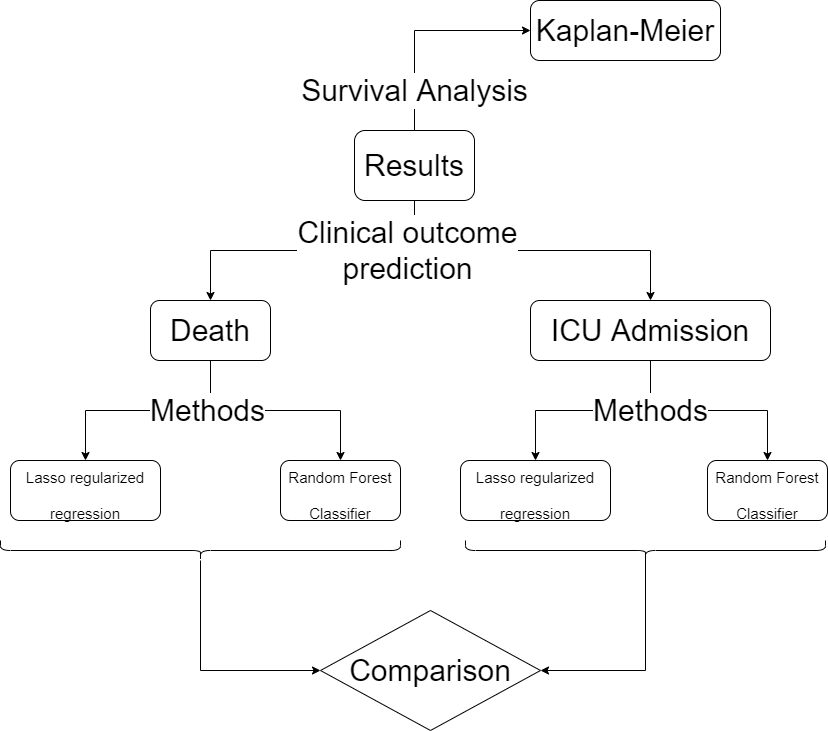
\includegraphics[width=1\textwidth]{Result_flowchart.png}
        \caption{Logical structure used in the presentation of the results.\label{ResultFlowchart}}
\end{figure}

\section{Predicting and classifying the outcome \death}
First step in reporting the results is going to be using \death as the clinical outcome of interest for either Lasso regularized regression or Random Forest classifier.

\subsection{Feature selection through Lasso regularization and clinical outcome prediction using regression}
When it comes to lasso regression usually graphs are reported that show the convergence of the parameters to the final value. Since the real information of this process is the value to which the coefficients converge only these values will be presented in tables and the ROC curves, with respective AUCs, will be provided. An example of the aforementione graph is the one visible in Figure \ref{LassoParam}.


\begin{figure}[htbp]
  		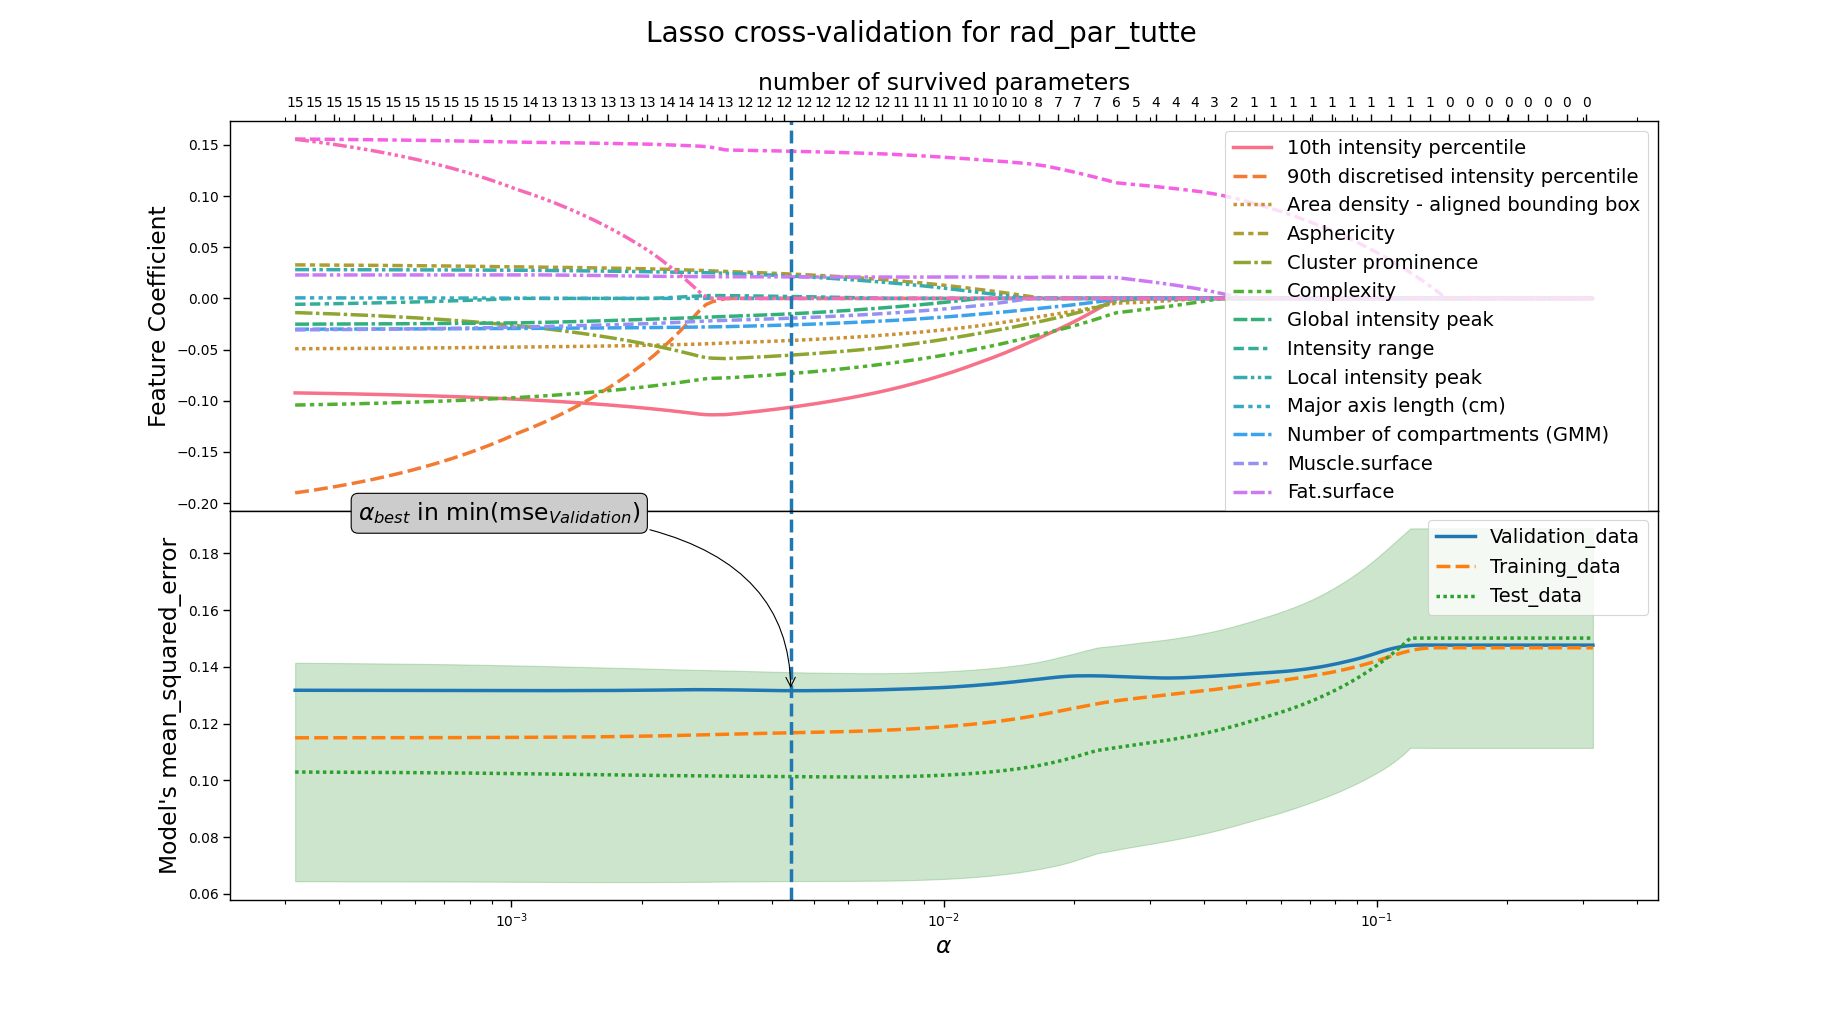
\includegraphics[width=1\textwidth]{Lasso_rad.png}
        \caption{Example of graph representing the convergence of the coefficients in a lasso procedure. The top graph represents how the values of the weights of the input features change as the Lasso hyperparameter $\alpha$ changes, the top axis label indicates at each point how many features would have weight different from zero. The bottom graph shows the curves that represent the behaviour of the mean squared error of the model on the validation set, the test set and the training set. One of the ways to find the optimal value of the $\alpha$ parameter is to find the value that minimizes the mean squared error relative to the validation set. The vertical dashed line is a graphical representation of how the values for the feature weight is chosen. This particular graph is relative to only radiomic features and comes from the regularization of a model that uses \death as target variable.\label{LassoParam}}
\end{figure}

Finally it seems useful to report Table \ref{tab:cont_tab} the contingency table that gives an idea on how superimposed the clinical outcomes on \death and \icu are.

\begin{table}
\caption{Contingency table that quantifies overlap between individual accessed in the ICU and Dead individuals.\label{tab:cont_tab}}
\centering
\begin{tabular}{l|rr}
\toprule
{} & \multicolumn{2}{l}{\icu} \\
 &       0 &   1 \\
\death&         &     \\
\midrule
0     &     311 &  47 \\
1     &      48 &  30 \\
\bottomrule
\end{tabular}
\end{table}

Starting to predict the death outcome, using Lasso regularized regression, of the patient different groups of features have been used, first of all only the radiomic features have been used. The ROC curve obtained with the radiomic features is the one in Figure \ref{RocDeathRad}. The curve in bold is an average curve obtained by aggregating the ten curves relative to each of the folds used in testing and the gray band represents a $\pm$ 1 standard deviation.

\begin{figure}[htbp]
	\centering
  		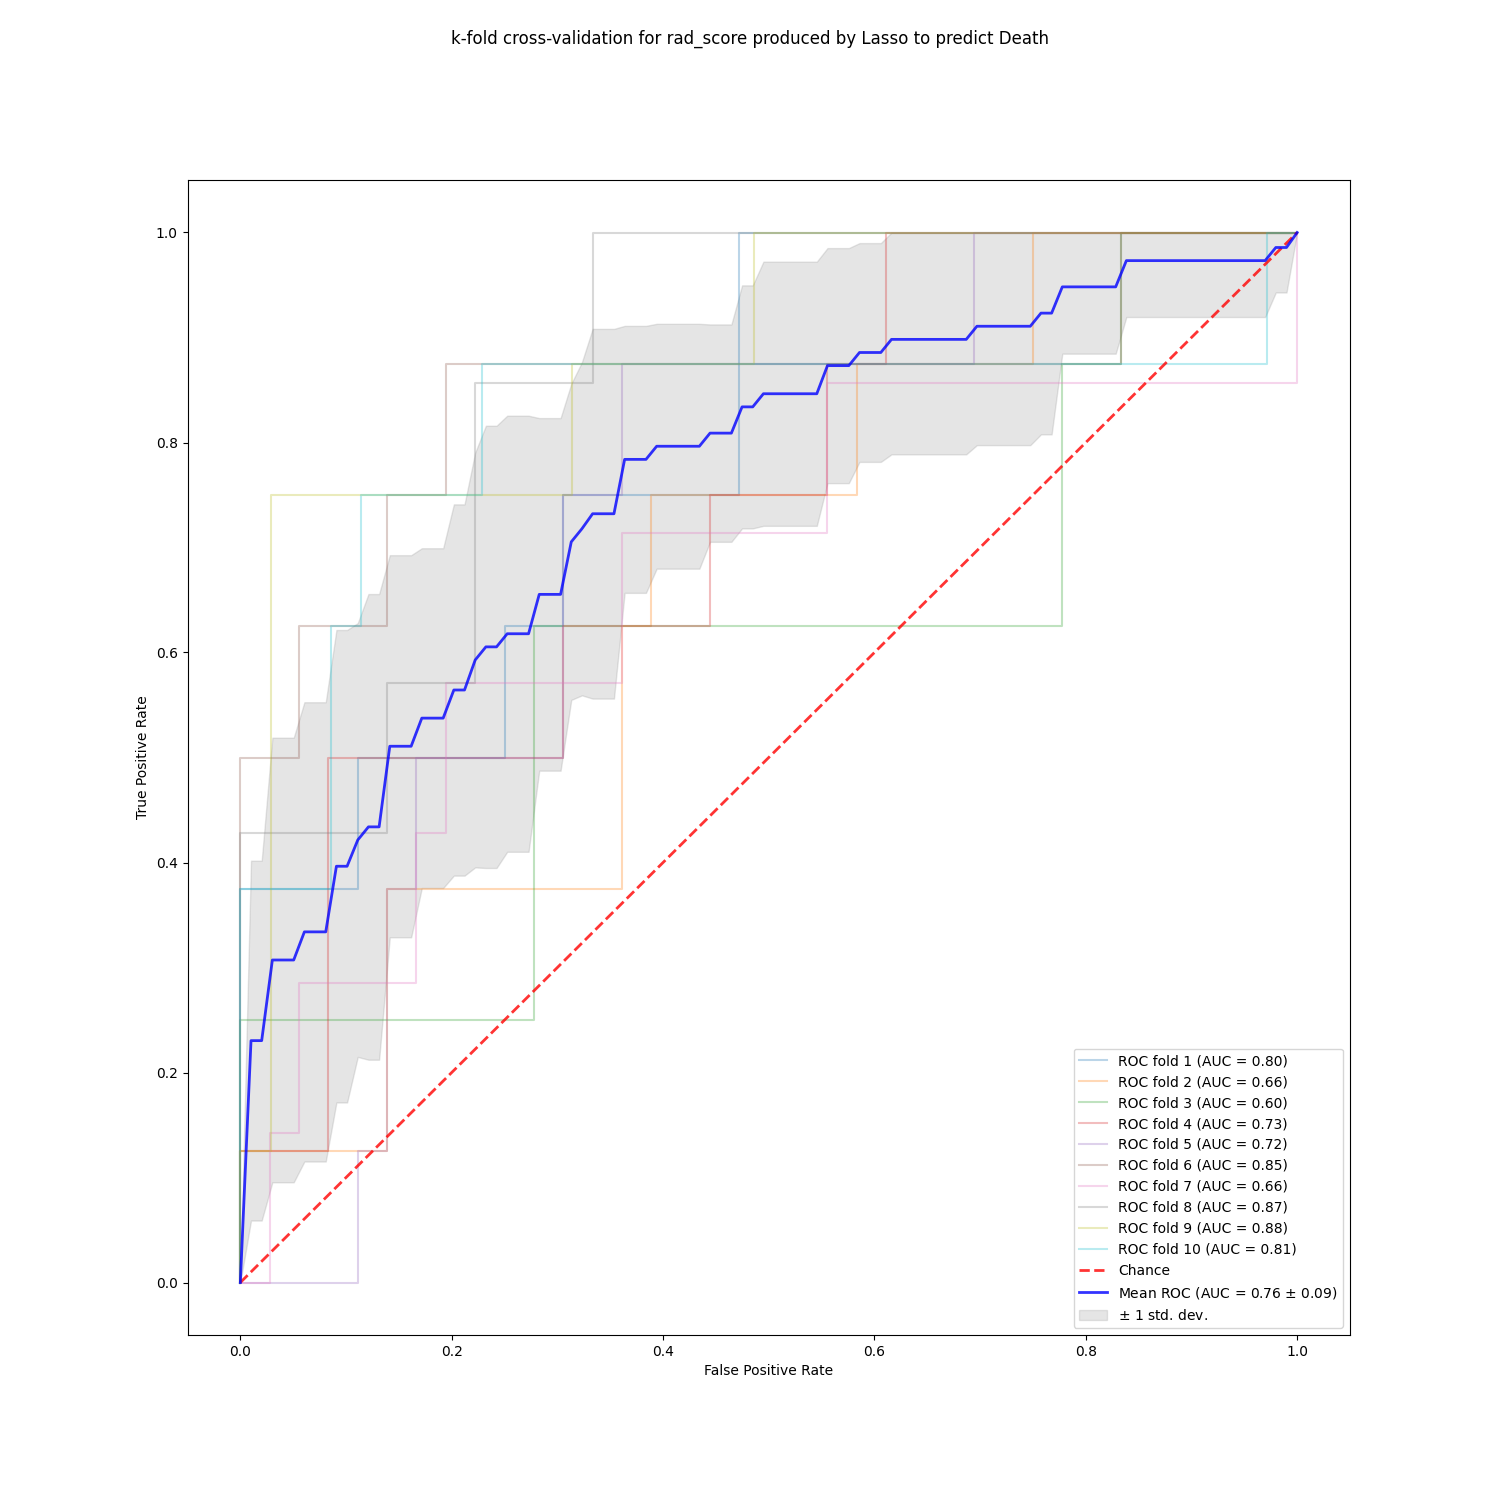
\includegraphics[scale=0.25]{ROC_CV_rad.png}
        \caption{ROC curves obtained with crossvalidation procedure using the radiomic features alone. In bold is the mean ROC with gray bands of width equal to the standard deviation. \label{RocDeathRad}}
\end{figure}

The model that was built using the coefficients reported in \ref{tab:ParamRad} reaches a AUC = 0.76$\pm$0.09. The features inside the tabular, as well as those in the tabulars that follow, will have the coefficients in descending order by absolute value so that the top features are the most relevant within it's relative model.

\begin{table}
\caption{Coefficients used in the linear combination estimated by a Lasso regularization relative to the radiomic features in modelling \death. All values are in descending order of absolute value\label{tab:ParamRad}}
\centering 
	\begin{tabular}{lr}
		\toprule
		Feature Name &   Importance \\
		\midrule
		Intercept                           &                      0.178899 \\
		10th intensity percentile           &                     -0.125094 \\
		Intensity-based interquartile range &                      0.103349 \\
		Complexity                          &                     -0.102924 \\
		Cluster prominence                  &                     -0.064690 \\
		Area density - aligned bounding box &                     -0.039374 \\
		Entropy                             &                      0.033002 \\
		Number of compartments (GMM)        &                     -0.032441 \\
		Asphericity                         &                      0.028517 \\
		Local intensity peak                &                      0.028478 \\
		Global intensity peak               &                     -0.024832 \\
		Intensity range                     &                      0.012509 \\
		Fat.surface                         &                      0.007267 \\
		Major axis length (cm)              &                      0.000000 \\
		Number of voxels of positive value  &                      0.000000 \\
		\bottomrule
	\end{tabular}
\end{table}

Before commenting more in depth the performance of this model it seems appropriate to see at least the other models built with singular features groups, so, when it comes to the clinical features, the results reported in Figure\ref{fig:RocDeathCli} and Table\ref{tab:ParamCli} have been obtained. All the results will be put together for ease in Table \ref{tab:RecapDeath}.

\begin{table}
\caption{Coefficients used in the linear combination estimated by a Lasso regularization relative to the clinical features in modelling \death. All values are in descending order of absolute value\label{tab:ParamCli}}
\centering
	\begin{tabular}{lr}
		\toprule
		Feature Name &   Importance \\
		\midrule
		Intercept          &                      0.178899 \\
		Age (years)        &                      0.116771 \\
		Respiratory Rate   &                      0.082292 \\
		Sex           &                     -0.037591 \\
		Febbre             &                     -0.022923 \\
		Hypertension       &                     -0.000000 \\
		History of smoking &                     -0.000000 \\
		Obesity            &                      0.000000 \\
		\bottomrule
	\end{tabular}
\end{table}

\begin{figure}[htbp]
	\centering
  		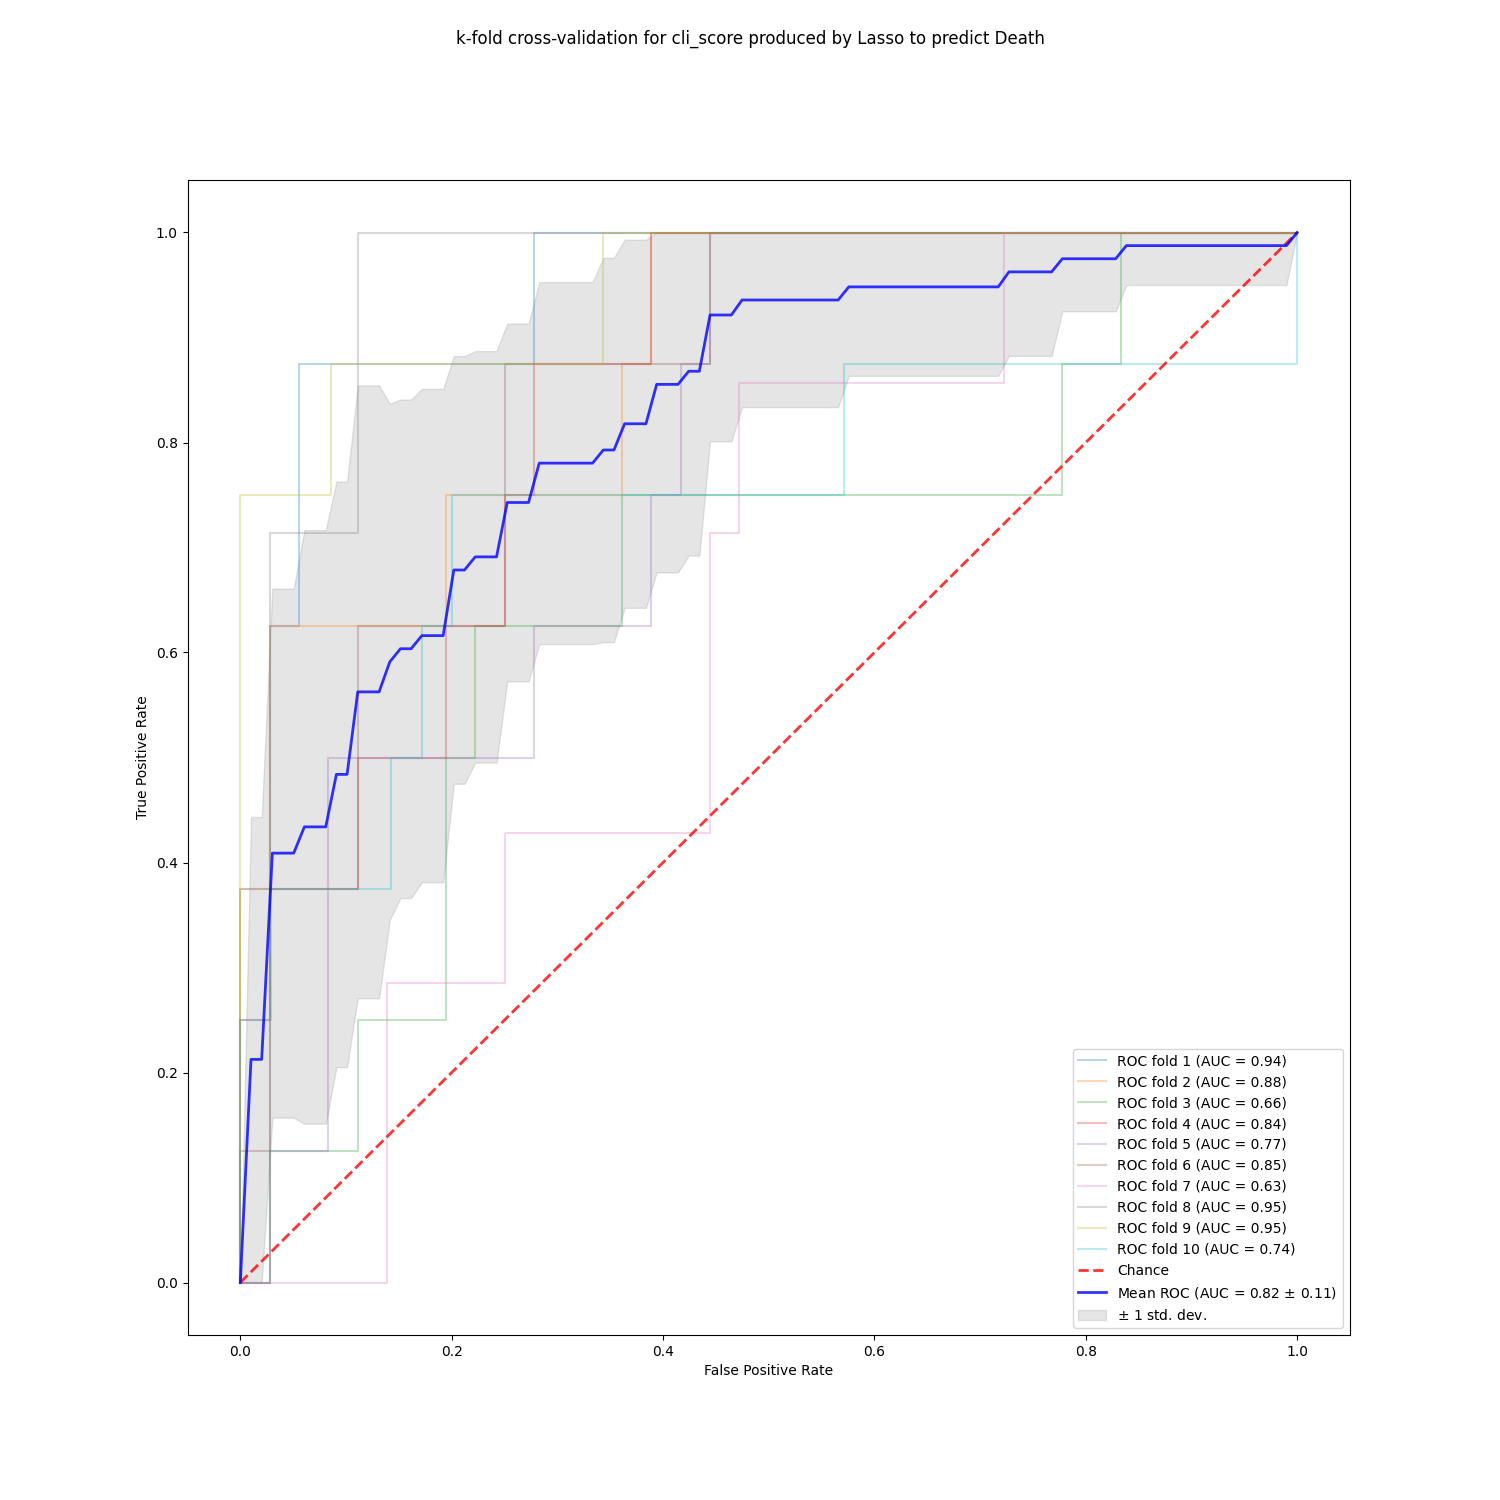
\includegraphics[scale=0.25]{ROC_CV_cli.png}
        \caption{ROC curves obtained with crossvalidation procedure using the clinical features alone. In bold is the mean ROC with gray bands of width equal to the standard deviation.\label{fig:RocDeathCli}}
\end{figure}

And finally, considering the radiological features Figure\ref{fig:RocDeathRadiologiche} and Table \ref{tab:ParamRadiologiche} are obtained.

\begin{table}
	\caption{Coefficients used in the linear combination estimated by a Lasso regularization on a linear regression model of death, relative to the radiological features. Values are in descending order of absolute value. \label{tab:ParamRadiologiche}}
		\centering
			\begin{tabular}{lr}
			\toprule
			Feature Name &  Importance \\
			\midrule
			Intercept             &                      0.178899 \\
			Ground-glass          &                     -0.043875 \\
			Lung consolidation    &                      0.038143 \\
			XRayTubeCurrent       &                     -0.017264 \\
			KVP                   &                      0.004995 \\
			Crazy Paving          &                     -0.000000 \\
			Bilateral Involvement &                      0.000000 \\
			SliceThickness        &                      0.000000 \\
			\bottomrule
			\end{tabular}
\end{table}

\begin{figure}[htbp]
	\centering
  		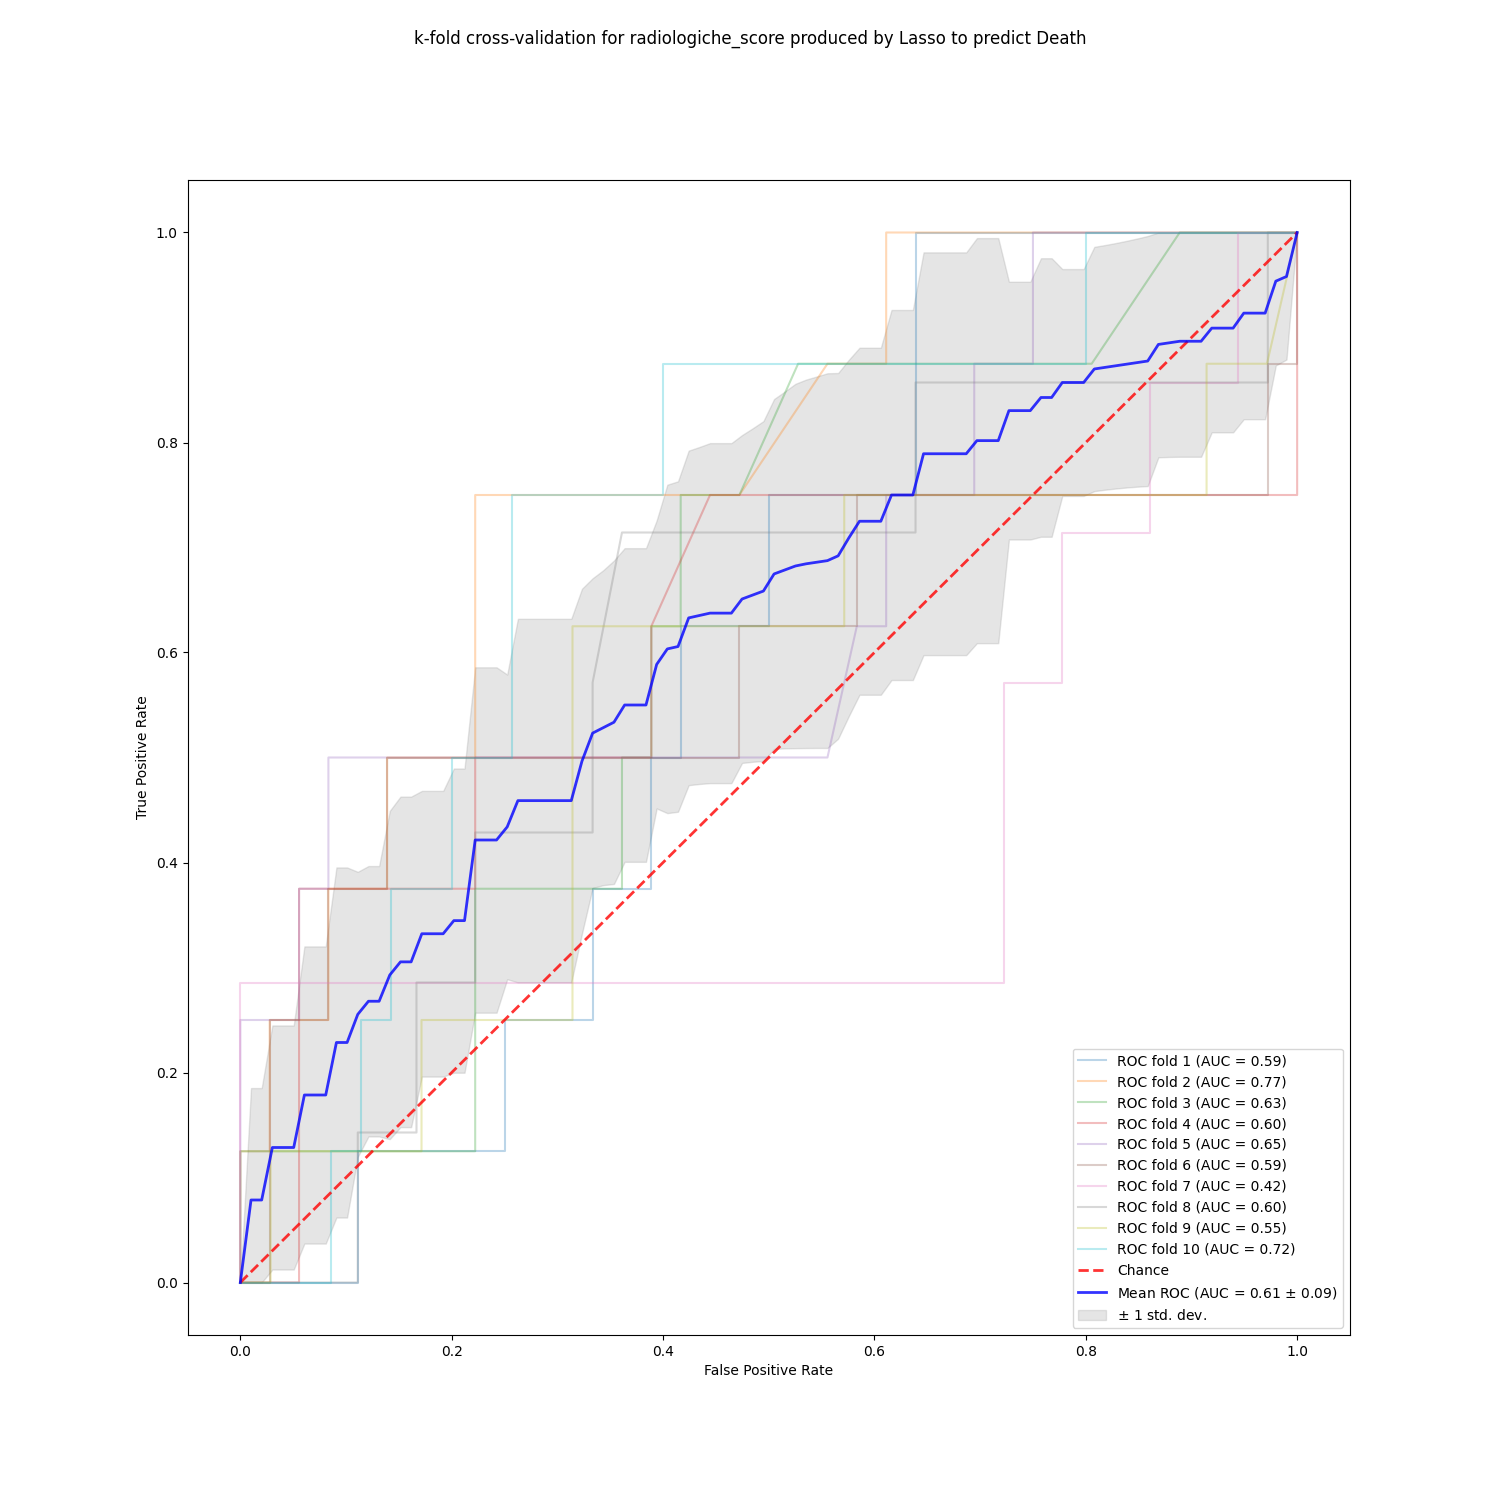
\includegraphics[scale=0.25]{ROC_CV_radiologiche.png}
        \caption{ROC curves obtained with crossvalidation procedure using the radiolocical features alone. As before  in bold is the mean ROC with bands of width equal to the standard deviation.\label{fig:RocDeathRadiologiche}}
\end{figure}

The first thing to notice is that the radiological features, when considered alone, have close to null predictive power. 
This is reasonable for at least part of the features because there is no reason for acquisition parameter to actually influence the outcome of the patient. 
 When it comes to the radiologically determined quantities, such as GGO, Crazy paving, lung consolidation and bilaterlaity even if one would expect these to be relevant their distribution across the dataset is not condusive the good predictions.
 In fact 88\% of patients had GGO, 50\% of all patient had Lung consolidation, 77\% of all patients did not have Crazy paving and 92\% had bilateral involvment.

When it comes to clinical features, category that performs better when considered singularly, nothing ground breaking has been obtained.
Age, Respiratory rate and sex are the most relevant features and are all very much in concordance with what is expected. Finally radiomic features perform slightly worse than the clinical features. To see if the feature obtained are, at least, reasonable a quick explanation is needed. 
This will be done only for the top performing features while deferring to \cite{IBSI} for the complete description:

\begin{itemize}
\item 10$^{th}$ intensity percentile and Intensity based interquartile range are both intensity based statistics.
\item Complexity: A complex image is one that presents many rapid changes in intensity and is heavily non-uniform because it has a lot of primitive components.
\item Cluster Prominence: GLCM feature which measures the symmetry and skewness of the matrix from which it derives. When this is high the image is not symmetric-
\item Area density aligned bounding box: This is a ratio of volume to surface.
\item Entropy: Measures the average quantity of information needed to describe the image. In other words it quantifies randomness in the image, the more random the more info is needed to describe it.
\end{itemize}

To summarize, since all of the features are computed on the whole lung segmentation, it seems that the some information on the distribution of gray levels as well as some textural information inside the whole lung are important.
It also seems that some information on the shape of the organ itself is also relevant.

One would expect that when combining all of the available features, i.e. by building a model using the previous clinical, radiomic and radiological features, the performance should somewhat rise especially given the fact that clinical and radiomic features have almost the same performance. The combined results can be seen in Figure \ref{fig:RocDeathAll} and Table \ref{tab:ParamAll}.

\begin{table}
	\caption{Coefficients used in the linear combination estimated by a Lasso regularization predicting death event relative to all available features features. Values are in descending order of absolute value\label{tab:ParamAll}}
		\centering
			\begin{tabular}{lr}
			\toprule
			Feature Name &  Importance \\
			\midrule
			Intercept                           &                      0.178899 \\
			Age (years)                         &                      0.092963 \\
			Intensity-based interquartile range &                      0.057260 \\
			Respiratory Rate                    &                      0.049603 \\
			Ground-glass                        &                     -0.031423 \\
			Sex\_bin                             &                     -0.028895 \\
			Complexity                          &                     -0.028606 \\
			Lung consolidation                  &                      0.017272 \\
			Febbre                              &                     -0.016933 \\
			XRayTubeCurrent                     &                     -0.016908 \\
			Area density - aligned bounding box &                     -0.009676 \\
			Cluster prominence                  &                     -0.006663 \\
			Fat.surface                         &                      0.004984 \\
			Number of compartments (GMM)        &                     -0.001448 \\
			Local intensity peak                &                      0.000195 \\
			Obesity                             &                      0.000000 \\
			Number of voxels of positive value  &                      0.000000 \\
			Hypertension                        &                      0.000000 \\
			Intensity range                     &                      0.000000 \\
			Global intensity peak               &                     -0.000000 \\
			Asphericity                         &                      0.000000 \\
			Crazy Paving                        &                     -0.000000 \\
			Bilateral Involvement               &                     -0.000000 \\
			SliceThickness                      &                      0.000000 \\
			KVP                                 &                      0.000000 \\
			10th intensity percentile           &                     -0.000000 \\
			Entropy                             &                      0.000000 \\
			History of smoking                  &                     -0.000000 \\
			\bottomrule
\end{tabular}
\end{table}

\begin{figure}[htbp]
	\centering
  		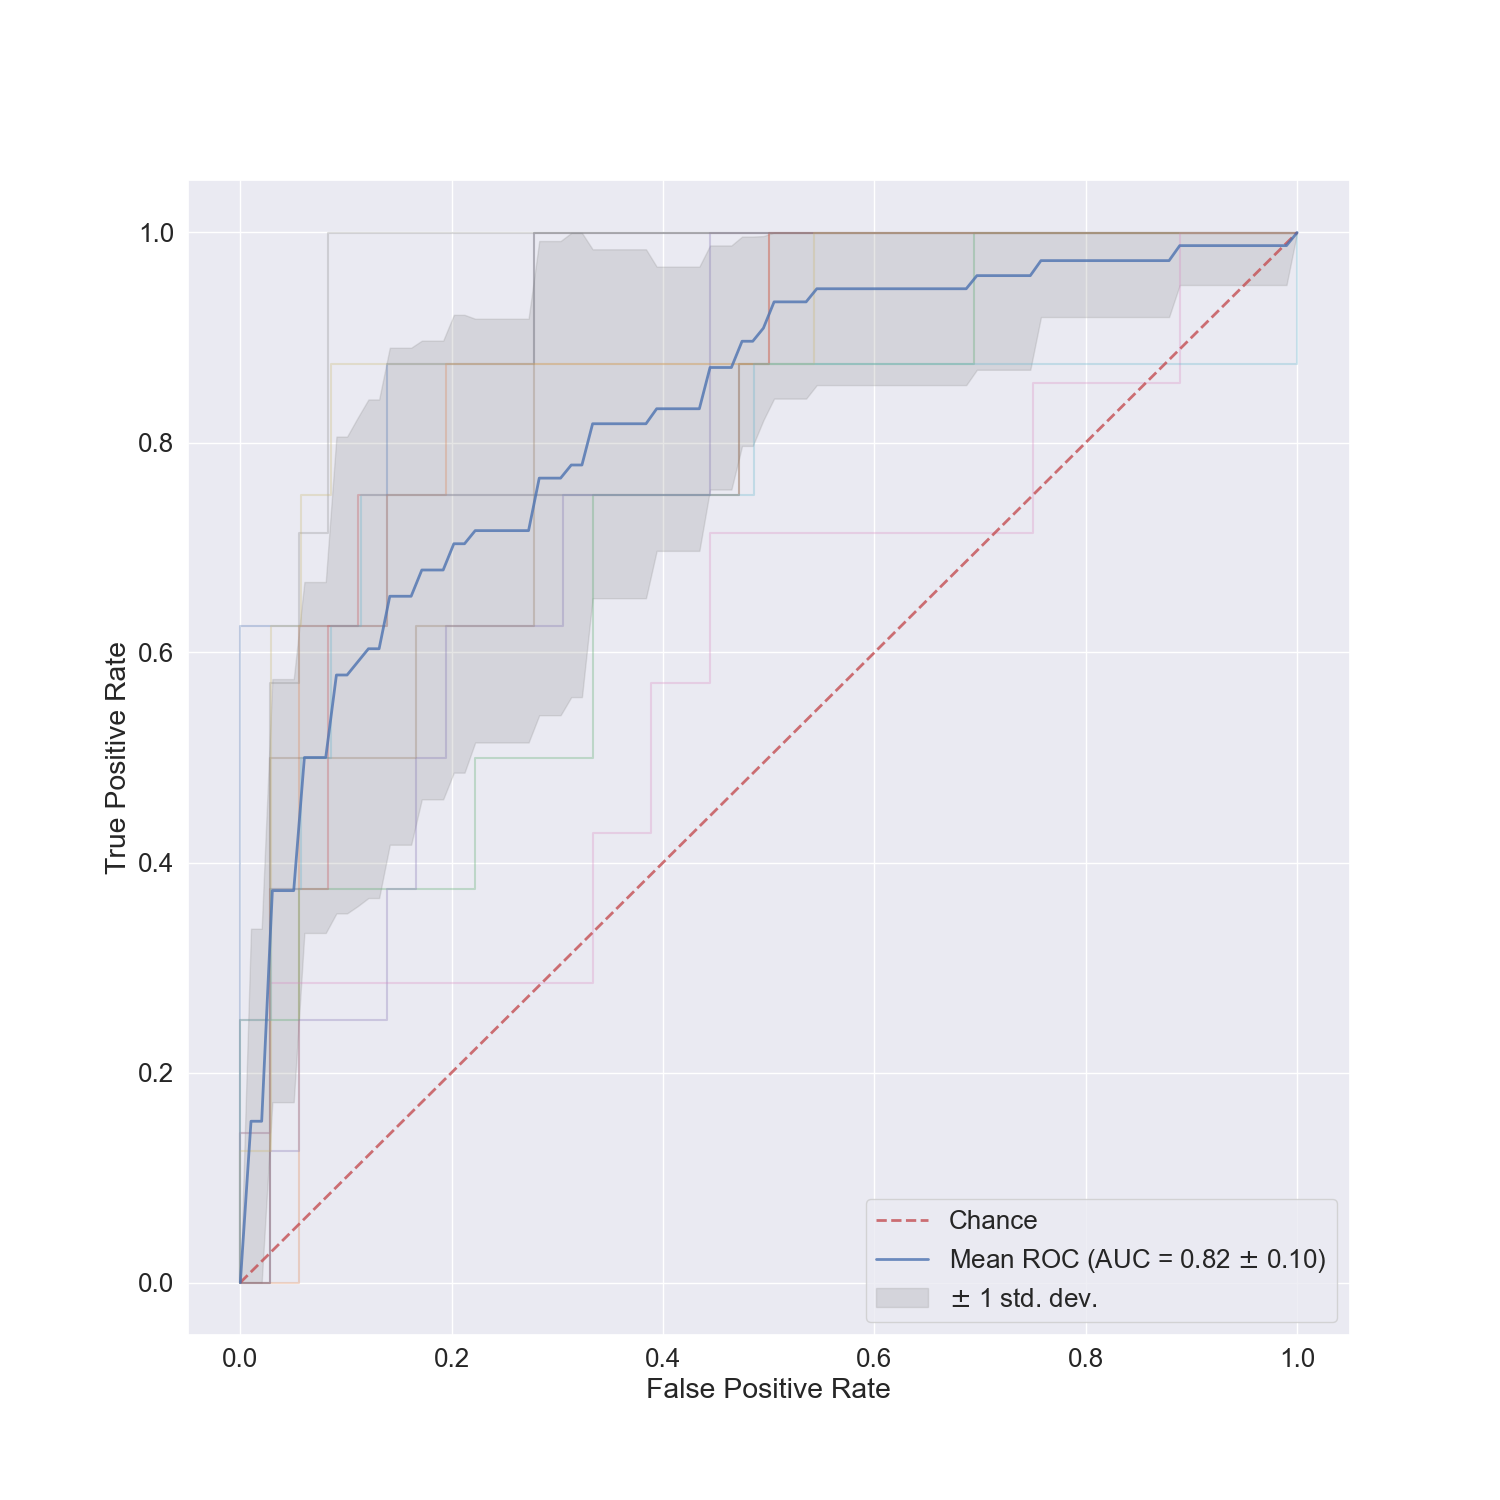
\includegraphics[scale=0.25]{ROC_CV_all.png}
        \caption{ROC curves obtained with crossvalidation procedure using all the available features. Model obtaine with Lasso regularization of a linear regression modelling death\label{fig:RocDeathAll}}
\end{figure}

In spite of what the expectations were, the performance of the combined case seems comparable if not equal to that obtained with clinical variables. To be sure of this claim a Delong test was used to compare pairwise the receiver operator curves and their respective AUCs. 

The null hypothesis of this test is that the two models are the same, hence a p-value smaller than 0.05 means that the curves and their AUCs are statistically different. The results from this analysis can be seen in \ref{fig:delongDeath}

\begin{table}
\caption{Recap table with the performance of the various models predicting on different groups of features predicting \death \label{tab:RecapDeath}}
\centering
\begin{tabular}{l|r}
\toprule
Features used & mean AUC $\pm$std\\
\midrule
Radiomic  & 0.76 $\pm$ 0.09\\
Clinical  &  0.82 $\pm$ 0.11\\
Radiological & 0.61 $\pm$ 0.09\\
All & 0.82 $\pm$ 0.10 \\
\bottomrule
\end{tabular}
\end{table}


\begin{figure}[H]
\centering
  	\subfloat[][Comparison clincal-radiomic]{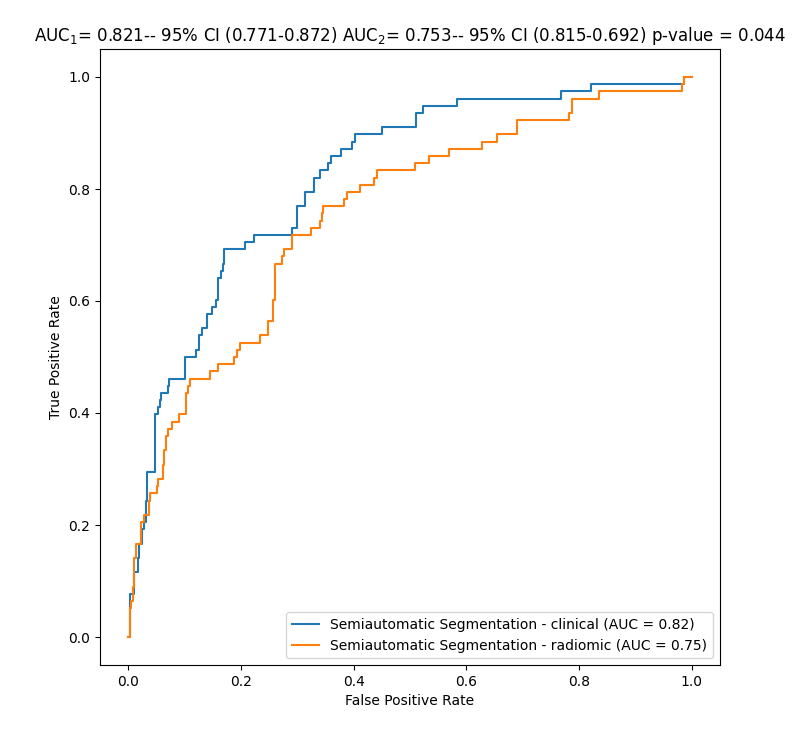
\includegraphics[width=0.50\linewidth]{Semi_CLIvsRAD_death.png}\label{fig:delongDeathCliRad}}
        \subfloat[][Comparison clinical-all]{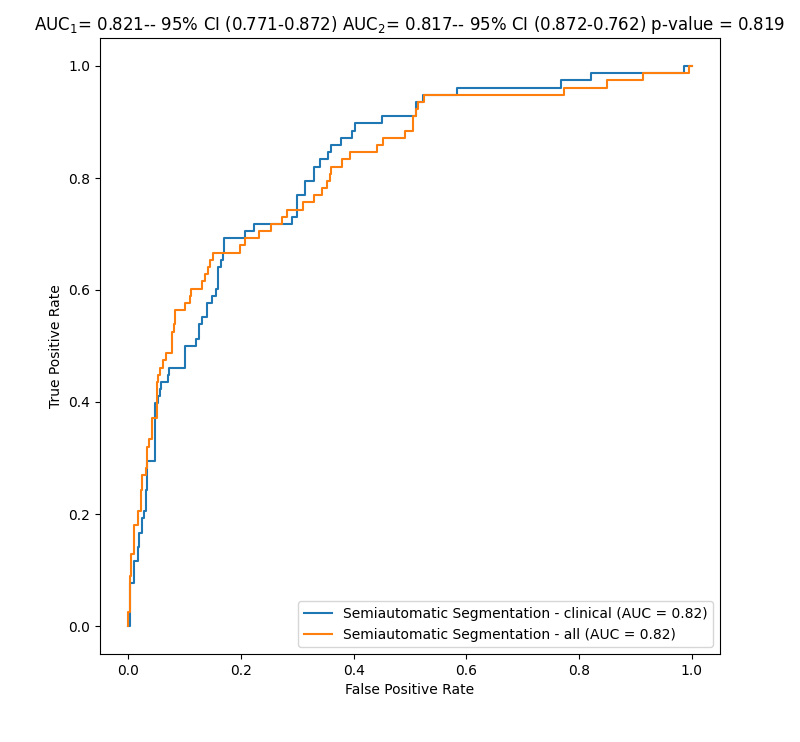
\includegraphics[width=0.50\linewidth]{Semi_CLIvsALL_death.png}\label{fig:delongDeathCliAll}}
        \caption{Comparison between ROC curves for clinical vs radiomic curves (a) and clinical vs all (b). The p-values are obtained with a Delong Test }\label{fig:delongDeath}
\end{figure}

As one would have expected the models from radiomic and clinical features are different while the ones built using clinical and all features are not statistically different.
Inspecting the coefficient of the parameters there are a few perplexing things to notice and a few reassuring ones. First of the reassuring facts is that the most relevant clinical features are still relevant in this combined model. 
Then, as one would expect, the radiological features retain some importance when combined with the others. However, when it comes to perplexing behaviours, the most concerning fact is that the radiomic features have mostly lost all relevance in the model which is surely unexpected.

Some possible explanations will be given in the concluding remarks at the end of this  subsection. as well as in the final chapter of the thesis.

\subsection{Classification of patients using Random forests}
For the sake of brevity all of the results will be reported and then discussed. Since RF classifiers use all of the availalble features it is very space consuming to report a table with all of the importances for the radiomic features as well as those used in the models with all the features. These two will be found in the appendix \ref{sec:RFAdditional} while those relative to clinical and radiological features will be reported here in Table \ref{tab:RFimpo}.

\begin{figure}[H]
\centering
  	\subfloat[][Radiomic Features]{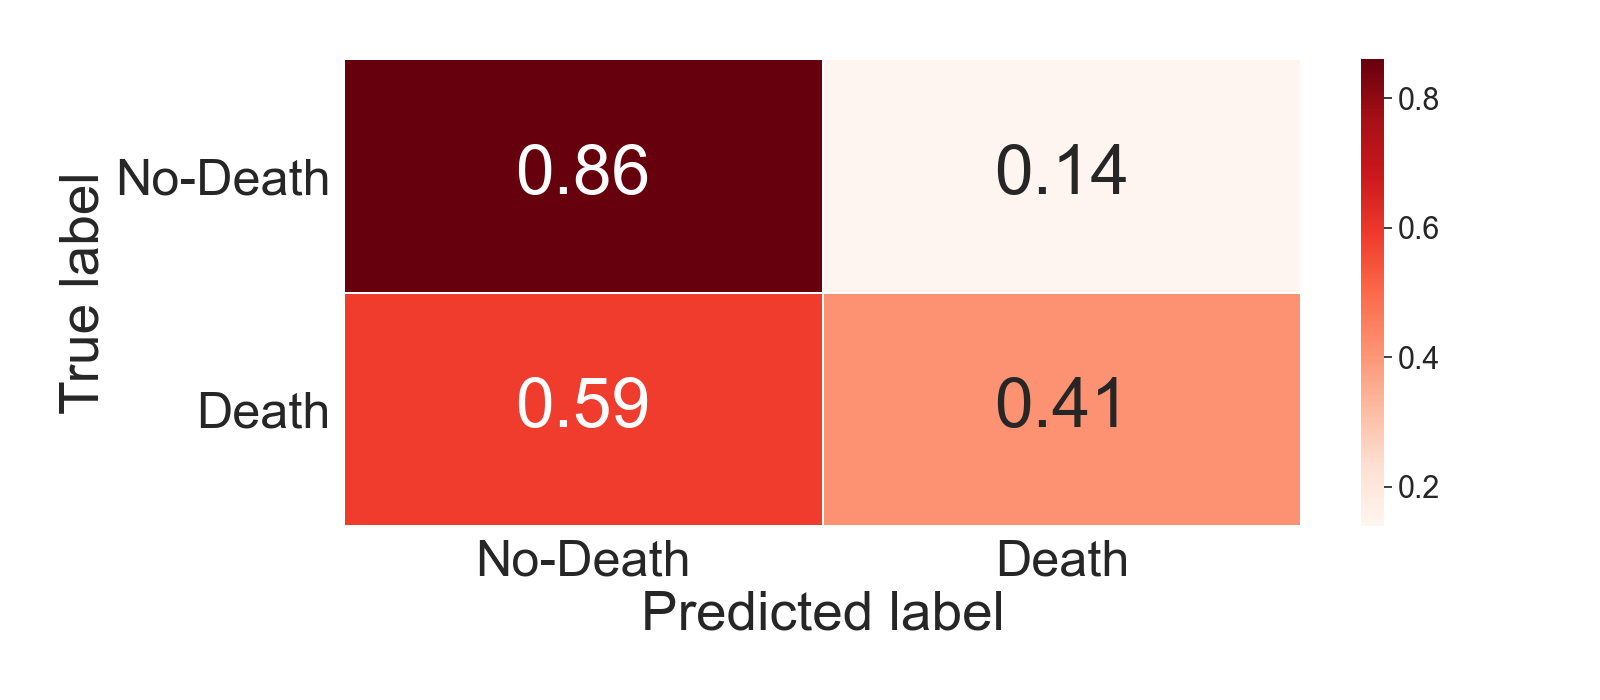
\includegraphics[width=0.50\linewidth]{Smote_Death_rad.png}\label{fig:RFDeathRad}}
        \subfloat[][Clinical Features]{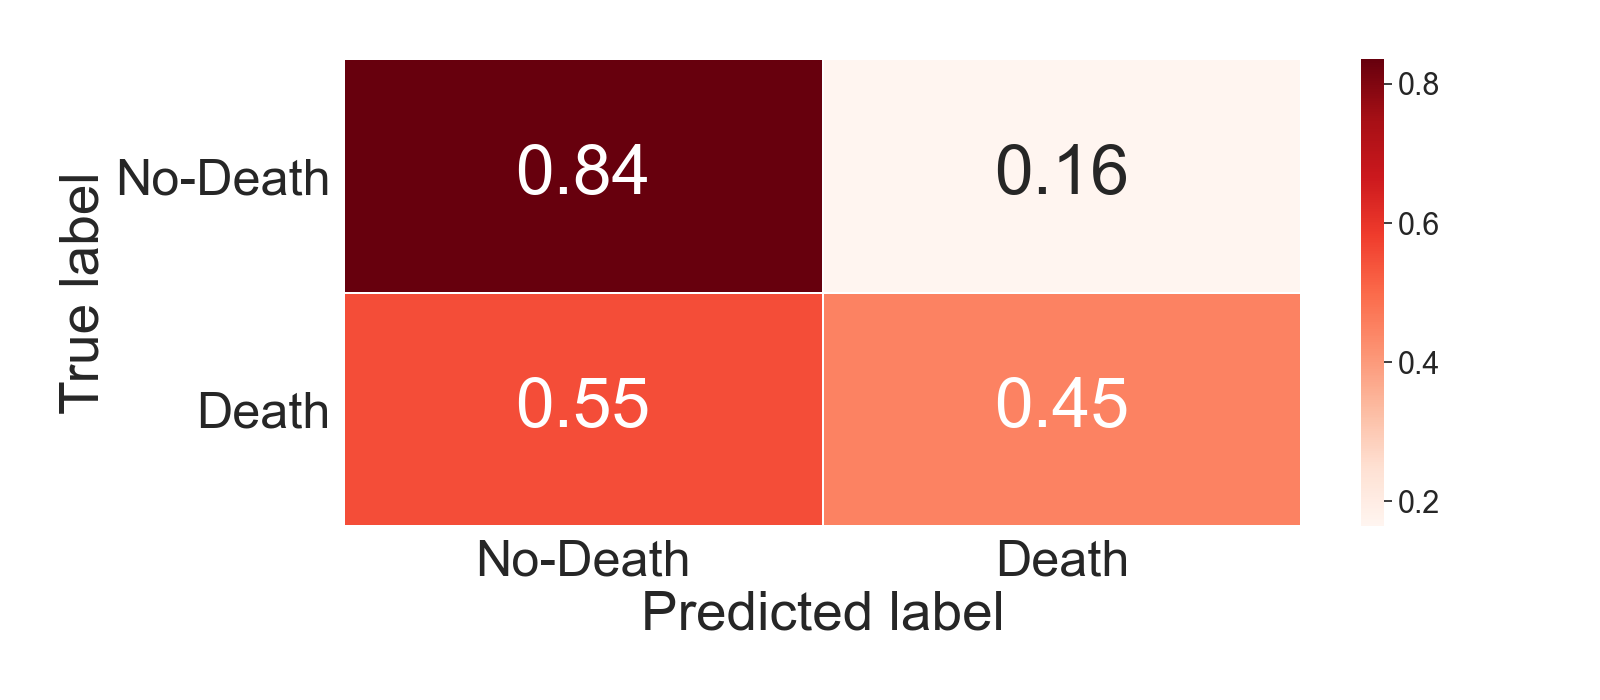
\includegraphics[width=0.50\linewidth]{Smote_Death_cli.png}\label{fig:RFDeathCli}}
	\newline
  	\subfloat[][Radiological Features]{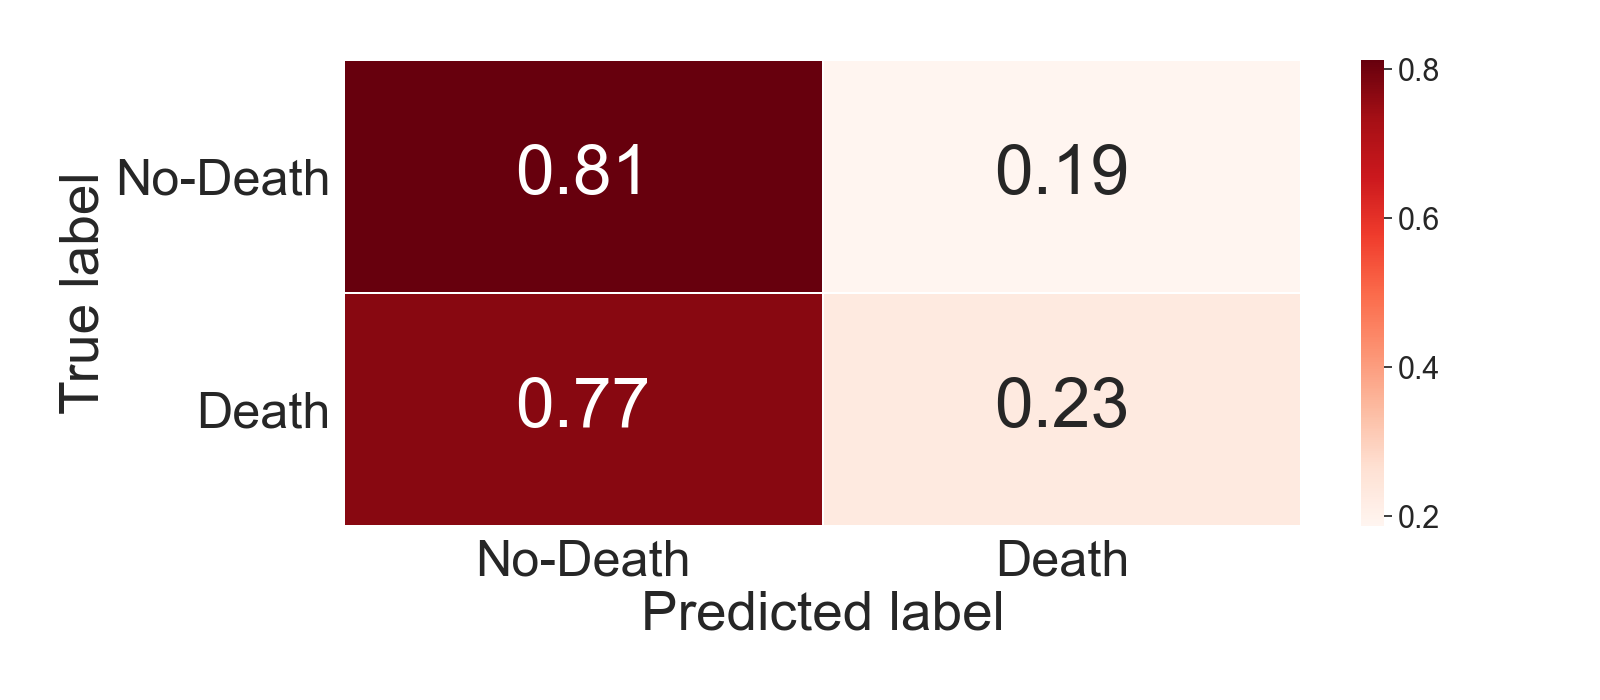
\includegraphics[width=0.50\linewidth]{Smote_Death_radiologiche.png}\label{fig:RFDeathRadiological}}
        \subfloat[][All Features]{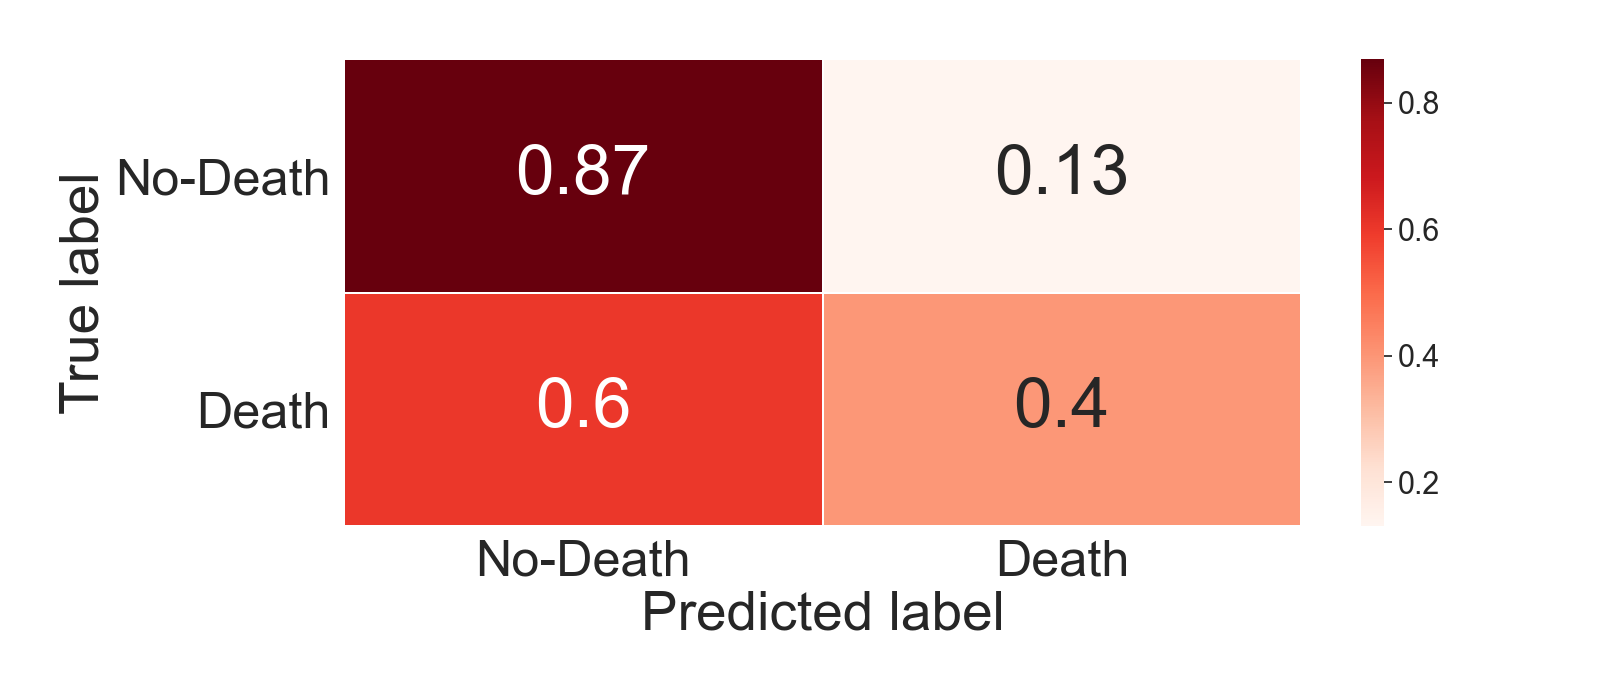
\includegraphics[width=0.50\linewidth]{Smote_Death_all.png}\label{fig:RFDeathAll}} 
        \caption{Confusion matrices for Random Forest cross-validated predictions after training on Synthetically oversampled data to predict \death. All of the available feature families are reported}\label{fig:RFDeath}
\end{figure}

Even without looking at the ROC curves it's plain to see that the data at hand is proving to be difficult for this model. Much like before radiological features alone are useless.
In evaluating these confusion matrices it should be kept in mind that the data is heavily unbalanced, since only $\sim$15\% of the patient died or were admitted in the ICU.
Even when using SMOTE in the training phase to correct this probelm it seems that the classifiers learns that it's optimal to guess that someone is alive. When it comes to the ROC curves Figure \ref{fig:RFDeathROC} and Table \ref{tab:RecapDeathRF} summarises the results.

\begin{figure}[H]
\centering
  	\subfloat[][Radiomic Features]{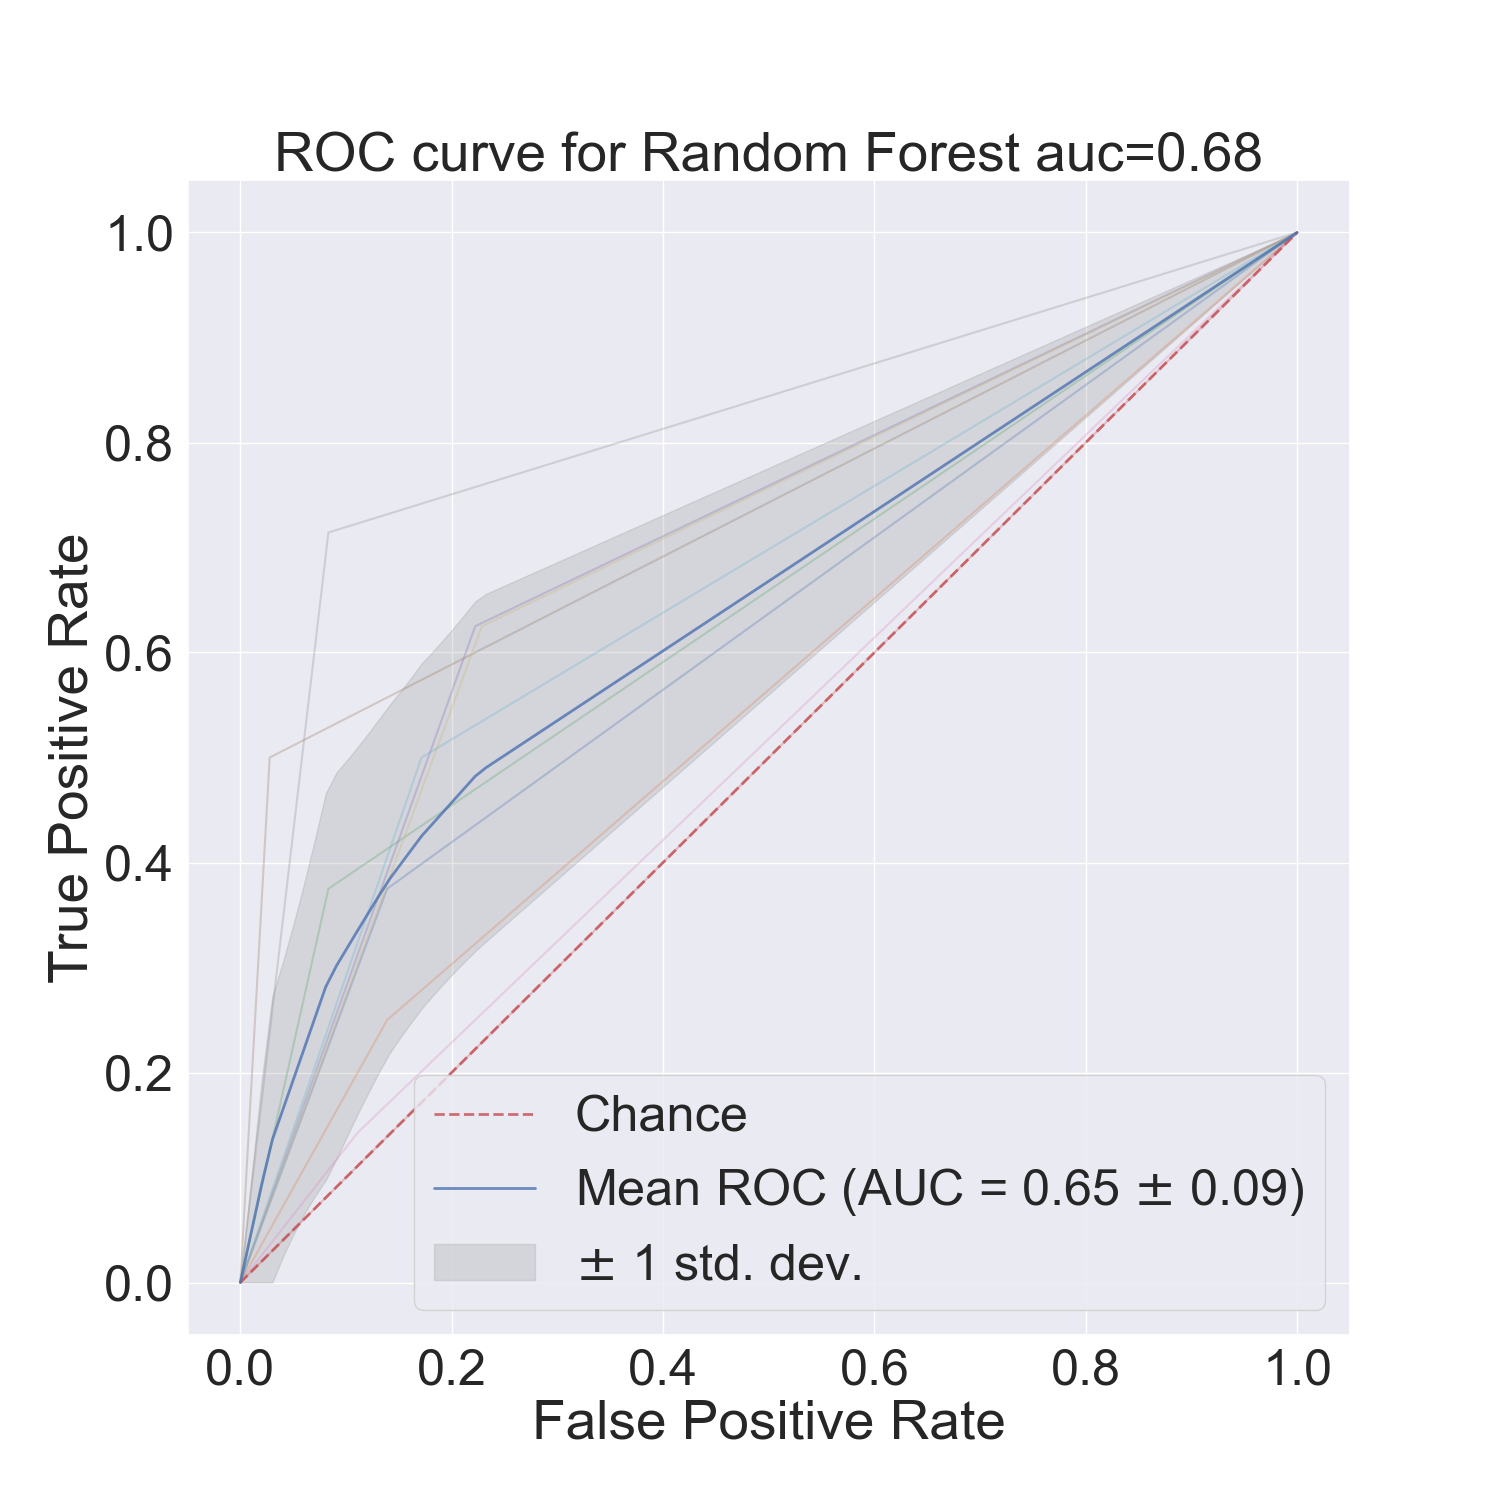
\includegraphics[width=0.50\linewidth]{SmoteROC_CV_Death_rad.png}\label{fig:RFDeathRadROC}}
        \subfloat[][Clinical Features]{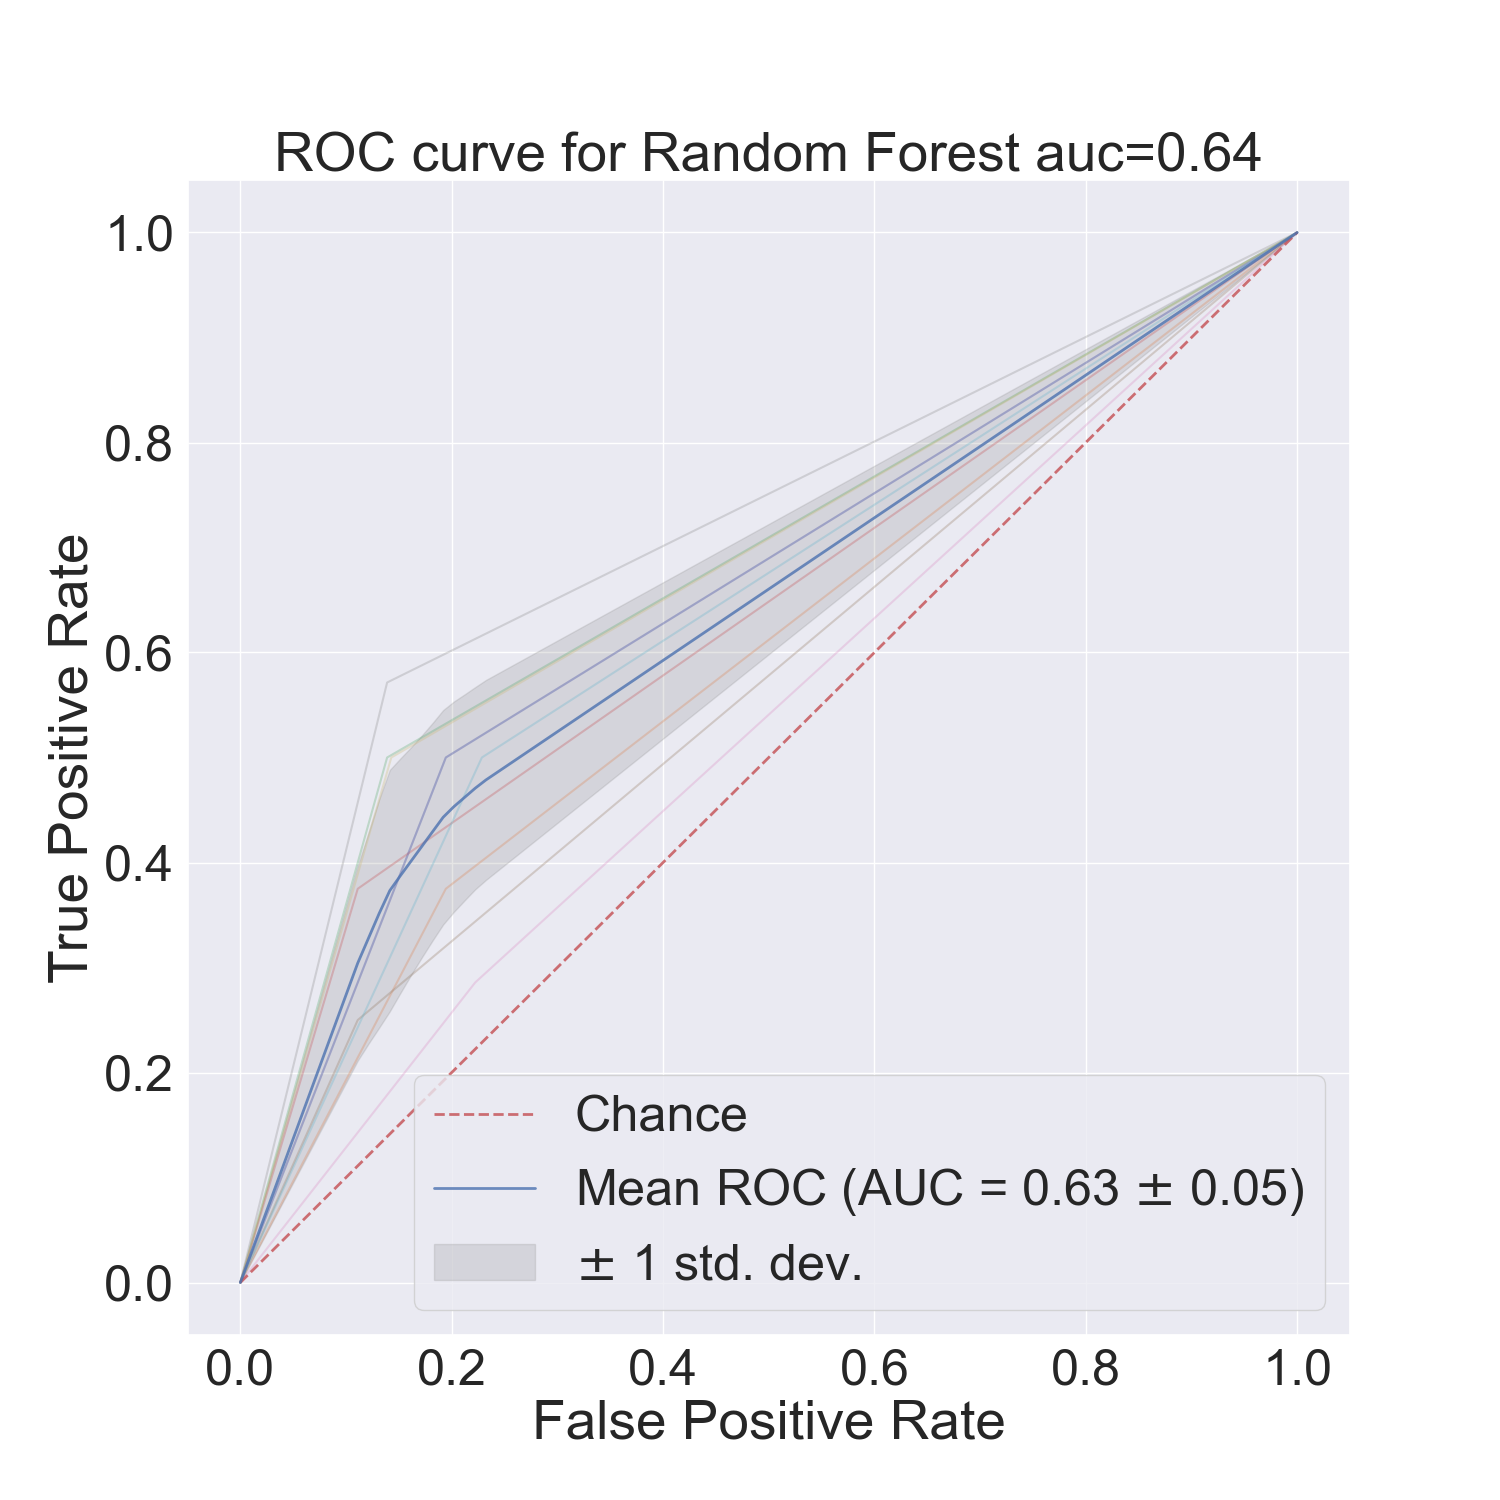
\includegraphics[width=0.50\linewidth]{SmoteROC_CV_Death_cli.png}\label{fig:RFDeathCliROC}}
	\newline
  	\subfloat[][Radiological Features]{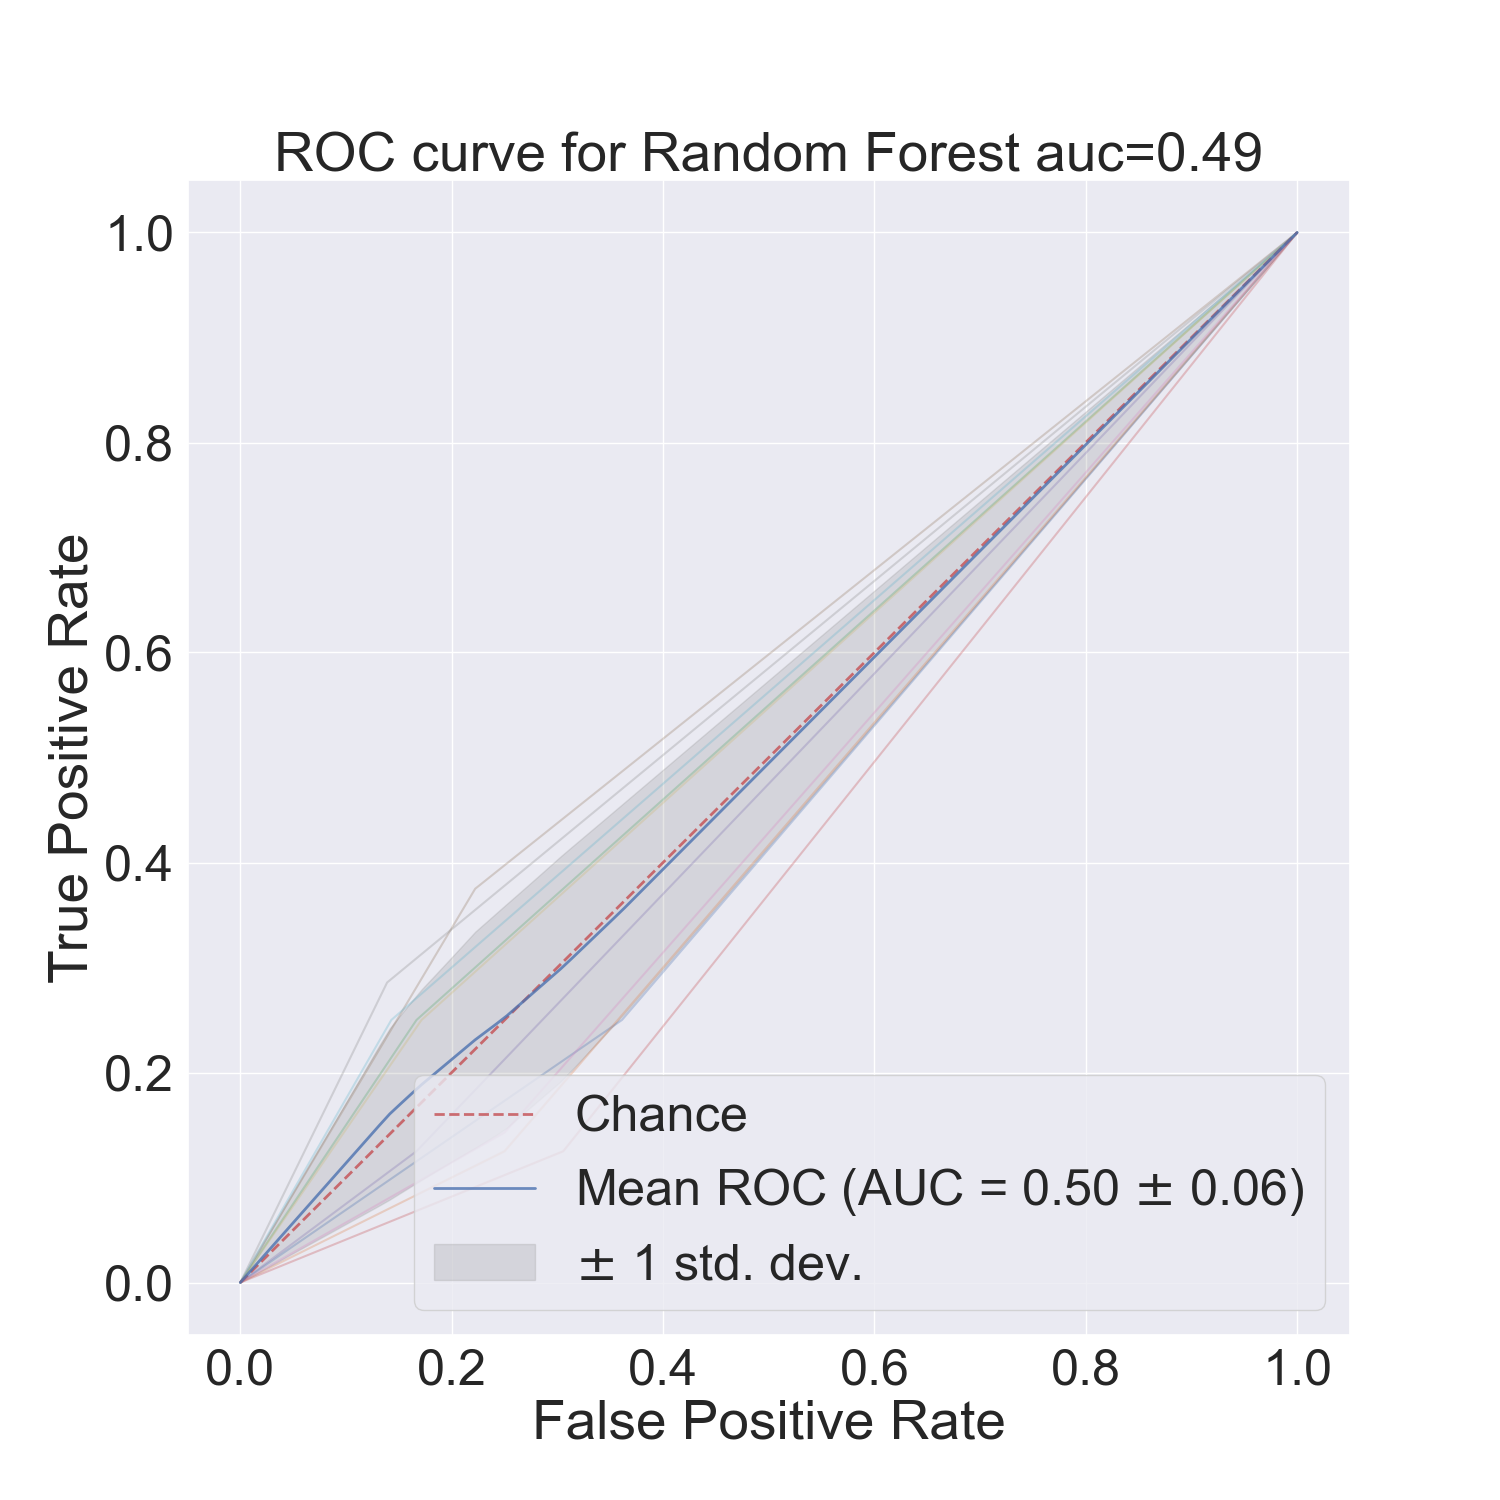
\includegraphics[width=0.50\linewidth]{SmoteROC_CV_Death_radiologiche.png}\label{fig:RFDeathRadiologicalROC}}
        \subfloat[][All Features]{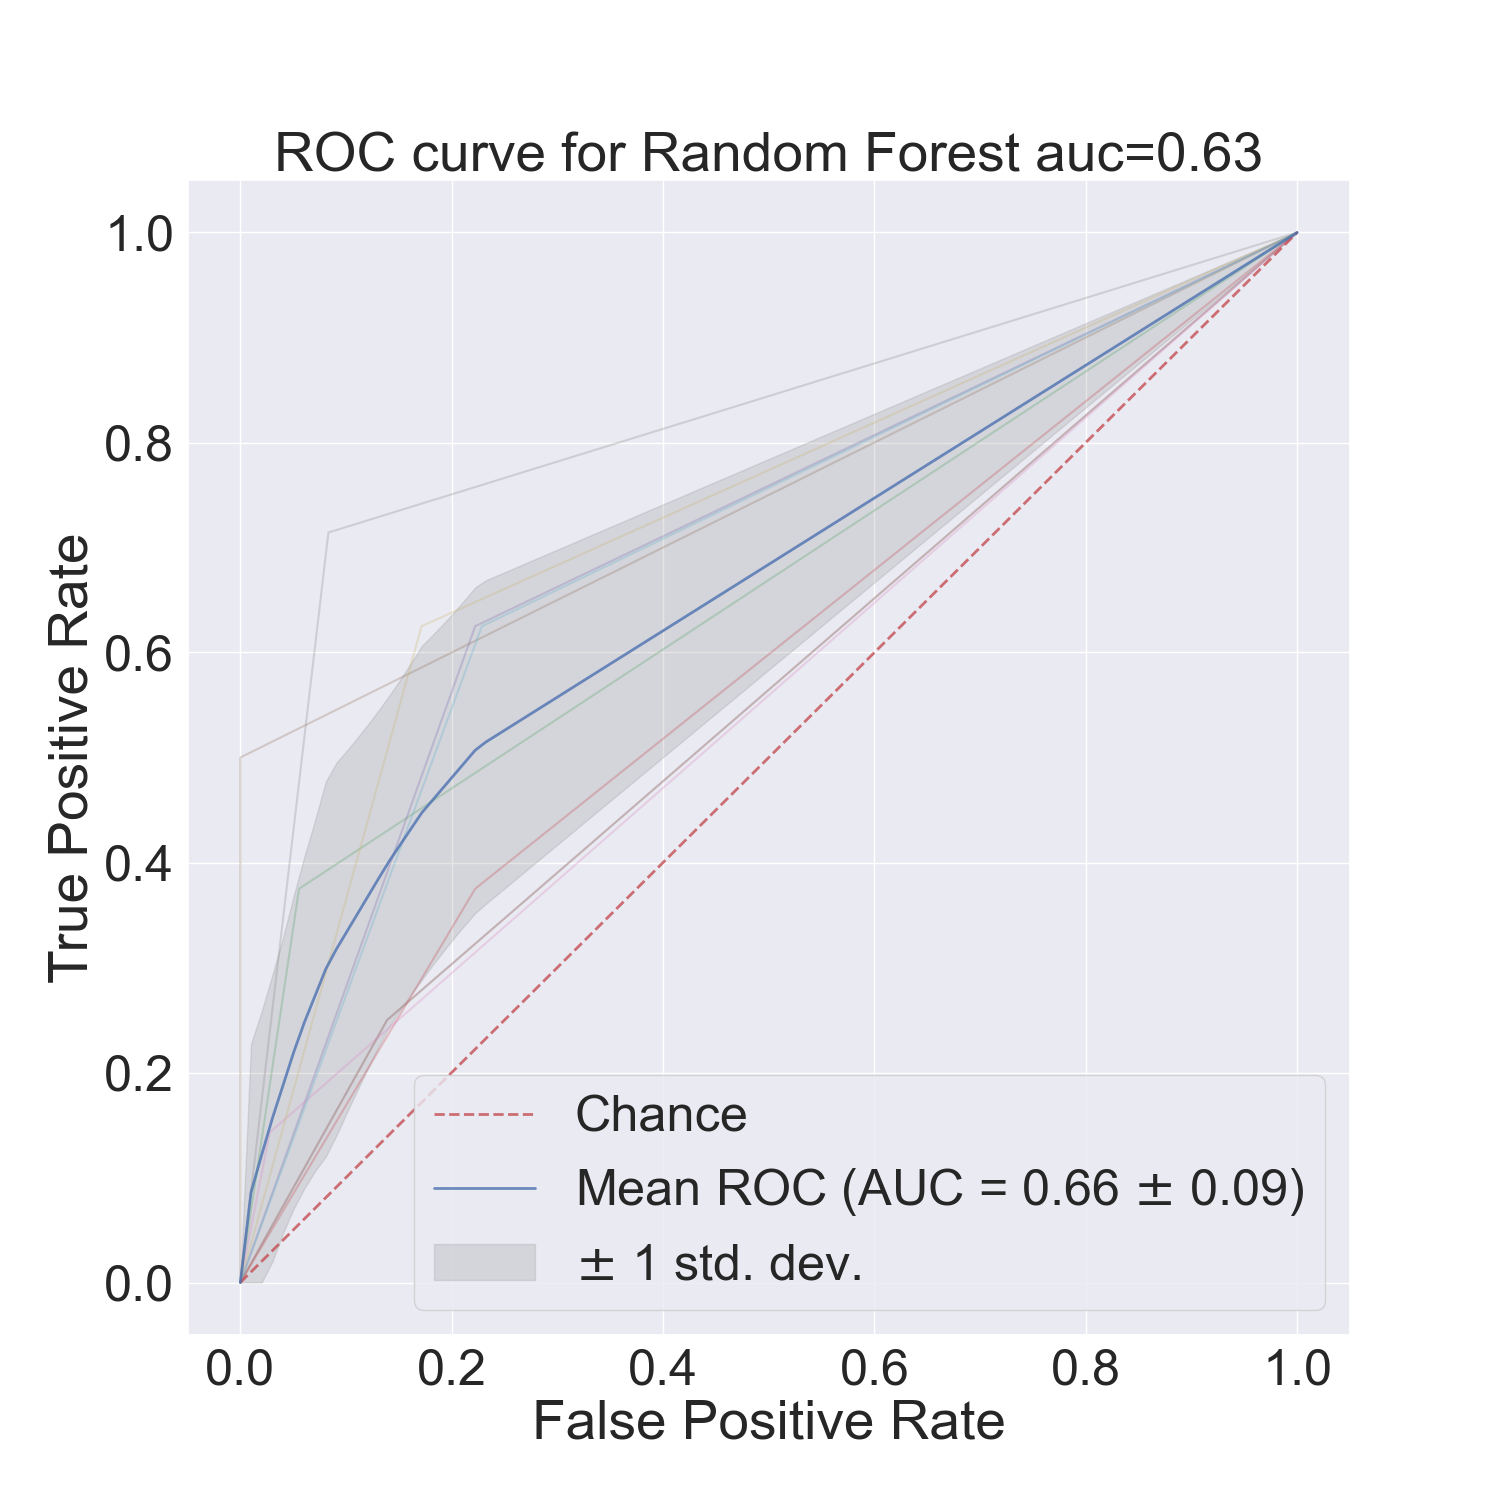
\includegraphics[width=0.50\linewidth]{SmoteROC_CV_Death_all.png}\label{fig:RFDeathAllROC}} 
        \caption{Cross-validated ROC curves built with Random forest classifier predictions of \death. Performances of allvariable families are reported }\label{fig:RFDeathROC}
\end{figure}

\begin{figure}[H]
\centering
  	\subfloat[][Radiological Features]{\begin{tabular}{lr}
				\toprule
				{} &  RF\_importances \\
				\midrule
				Age (years)        &        0.463821 \\
				Respiratory Rate   &        0.287735 \\
				Febbre             &        0.084276 \\
				Sex\_bin            &        0.079571 \\
				Hypertension       &        0.033435 \\
				History of smoking &        0.029404 \\
				Obesity            &        0.021758 \\
				\bottomrule
				\end{tabular}
							}
        \subfloat[][Clinical Features]{
			\begin{tabular}{lr}
				\toprule
				{} &  RF\_importances \\
				\midrule
				XRayTubeCurrent       &        0.800101 \\
				Lung consolidation    &        0.043942 \\
				KVP                   &        0.039768 \\
				Crazy Paving          &        0.032511 \\
				SliceThickness        &        0.031362 \\
				Ground-glass          &        0.030423 \\
				Bilateral Involvement &        0.021893 \\
				HRCT performed        &        0.000000 \\
				\bottomrule
			\end{tabular}
							}
        \caption{Importances estimated by random forest}\label{fig:RFimpo}
\end{figure}


\begin{table}
\caption{Recap table with the performance of the various families of features \label{tab:RecapDeathRF}}
\centering
\begin{tabular}{l|r}
\toprule
Features used & mean AUC $\pm$std\\
\midrule
Radiomic  & 0.65 $\pm$ 0.13\\
Clinical  &  0.64 $\pm$ 0.06\\
Radiological & 0.50 $\pm$ 0.07\\
All & 0.66 $\pm$ 0.8 \\
\bottomrule
\end{tabular}
\end{table}

Once again the curves are evidently not statistically different. This counterintuitive behaviour seems to be constant across the two implemented methods and also across different labels tried. An attempt to explain this phenomenon will be postponed to the next chapter


\section{Predicting and classifying the outcome \icu}
The second step in reporting the results is the comparison of the methods used to predict \icu as clinical outcome.

\subsection{Feature selection through Lasso regularization and clinical outcome prediction using regression}

In trying to predict if the patient will be admitted in the Intensive Care Unit of the hospital the same procedure as before has been used. The ROC curves obtained with the various features are reported in Figure \ref{fig:ICULasso}. Just like before the curve in bold is an average curve obtained by aggregating the ten curves relative to each of the folds used in testing and the gray band represents a $\pm$ 1 standard deviation.
Following the blueprint of the previous subsection, all of the results will be presented and then briefly discussed


\begin{figure}[H]
\centering
  	\subfloat[][Radiomic Features]{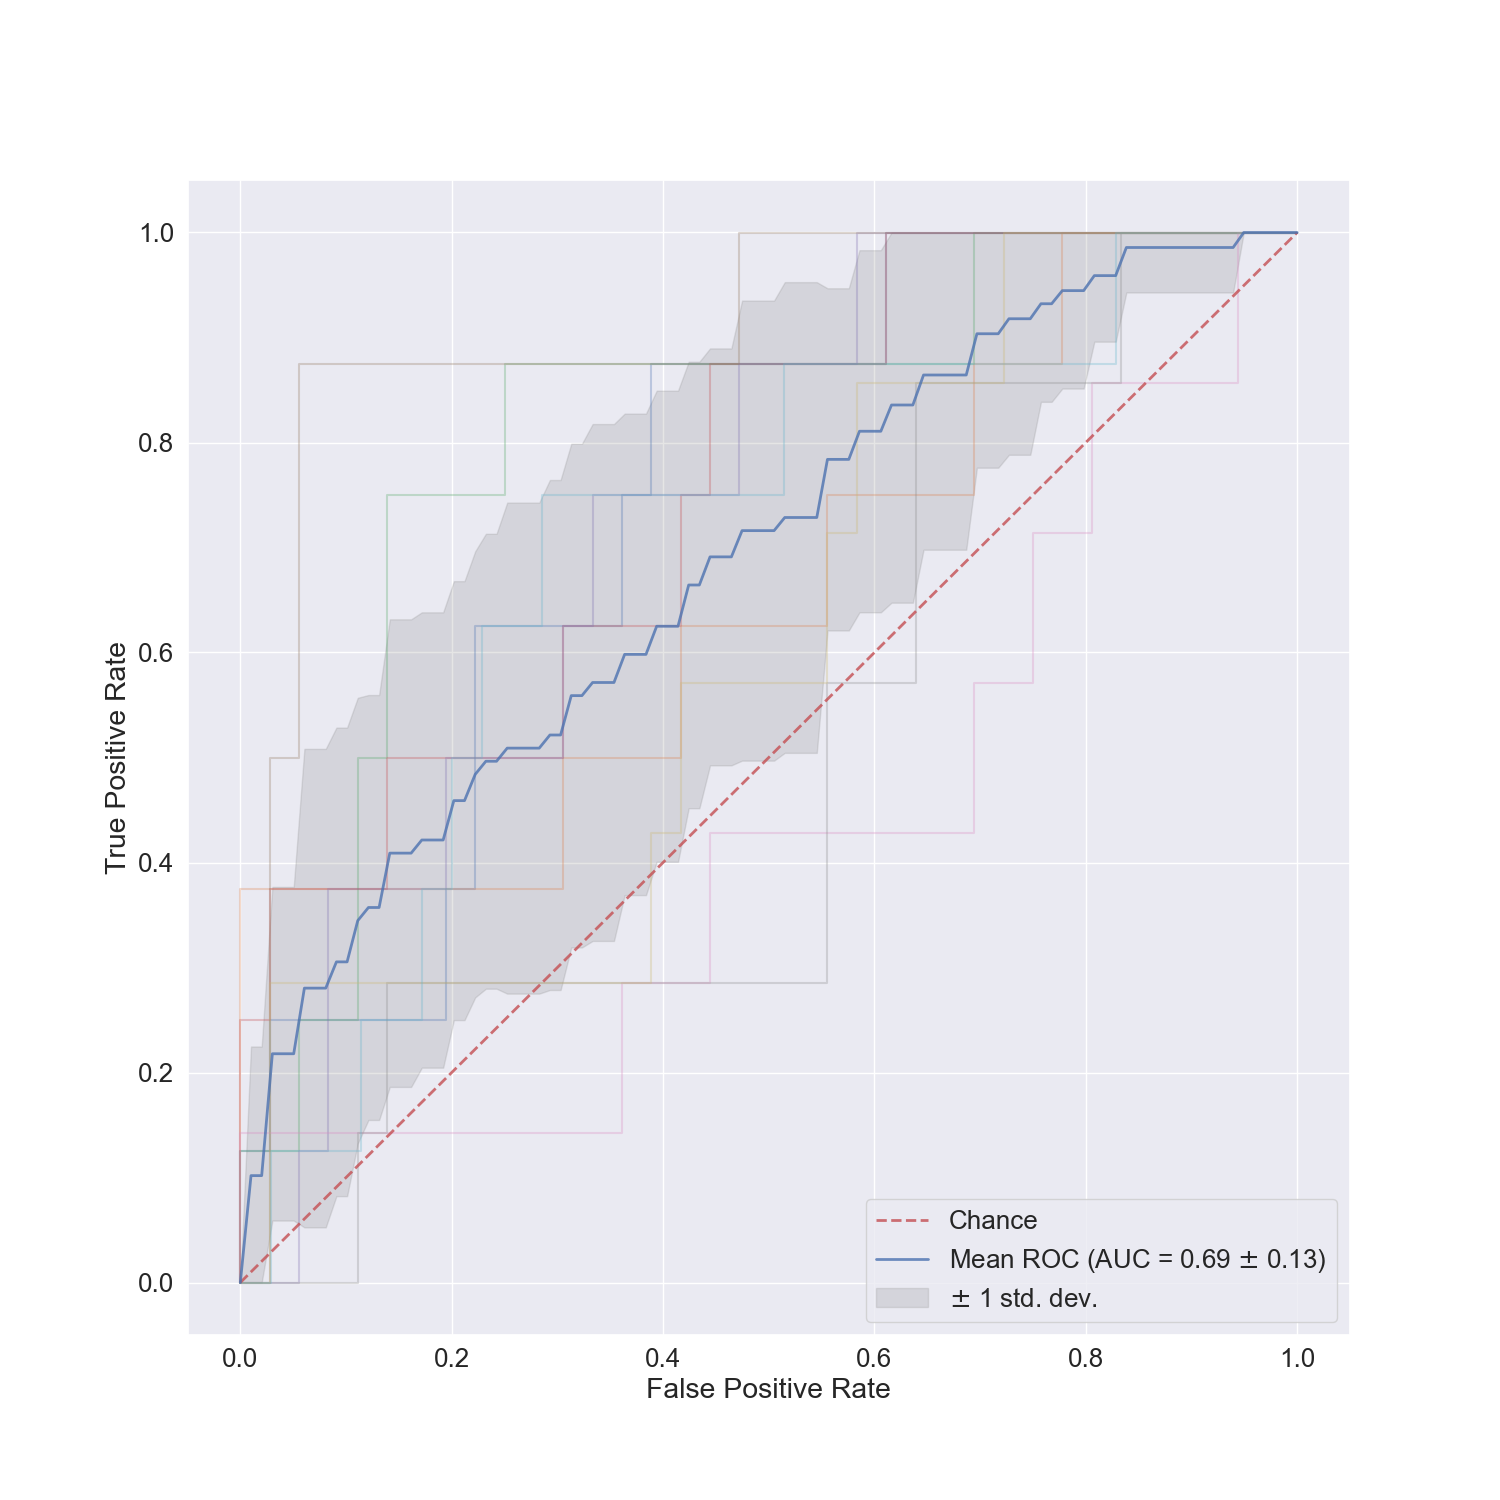
\includegraphics[width=0.50\linewidth]{ROC_CV_rad_icu.png}\label{fig:ROCICUrad}}
        \subfloat[][Clinical Features]{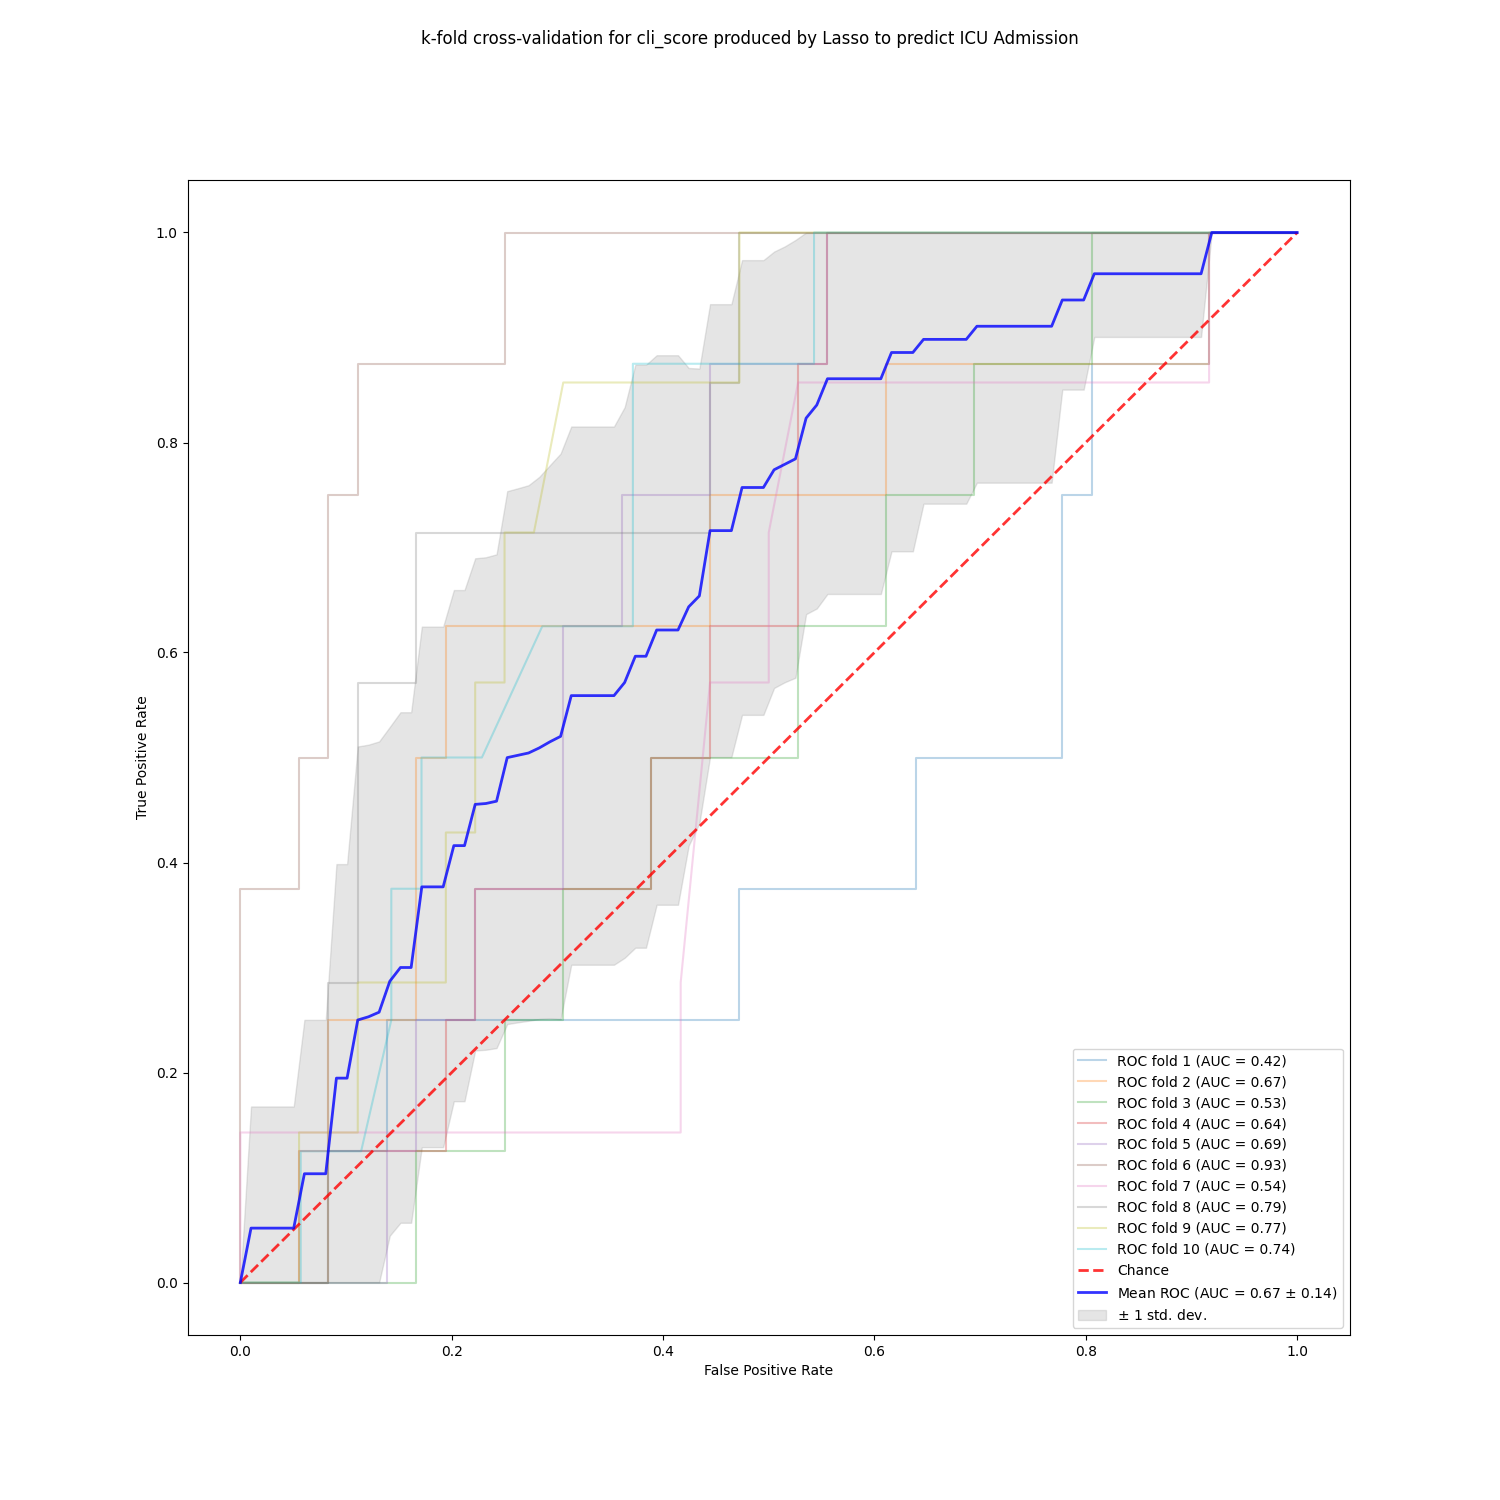
\includegraphics[width=0.50\linewidth]{ROC_CV_cli_icu.png}\label{fig:ROCICUcli}}
	\newline
  	\subfloat[][Radiological Features]{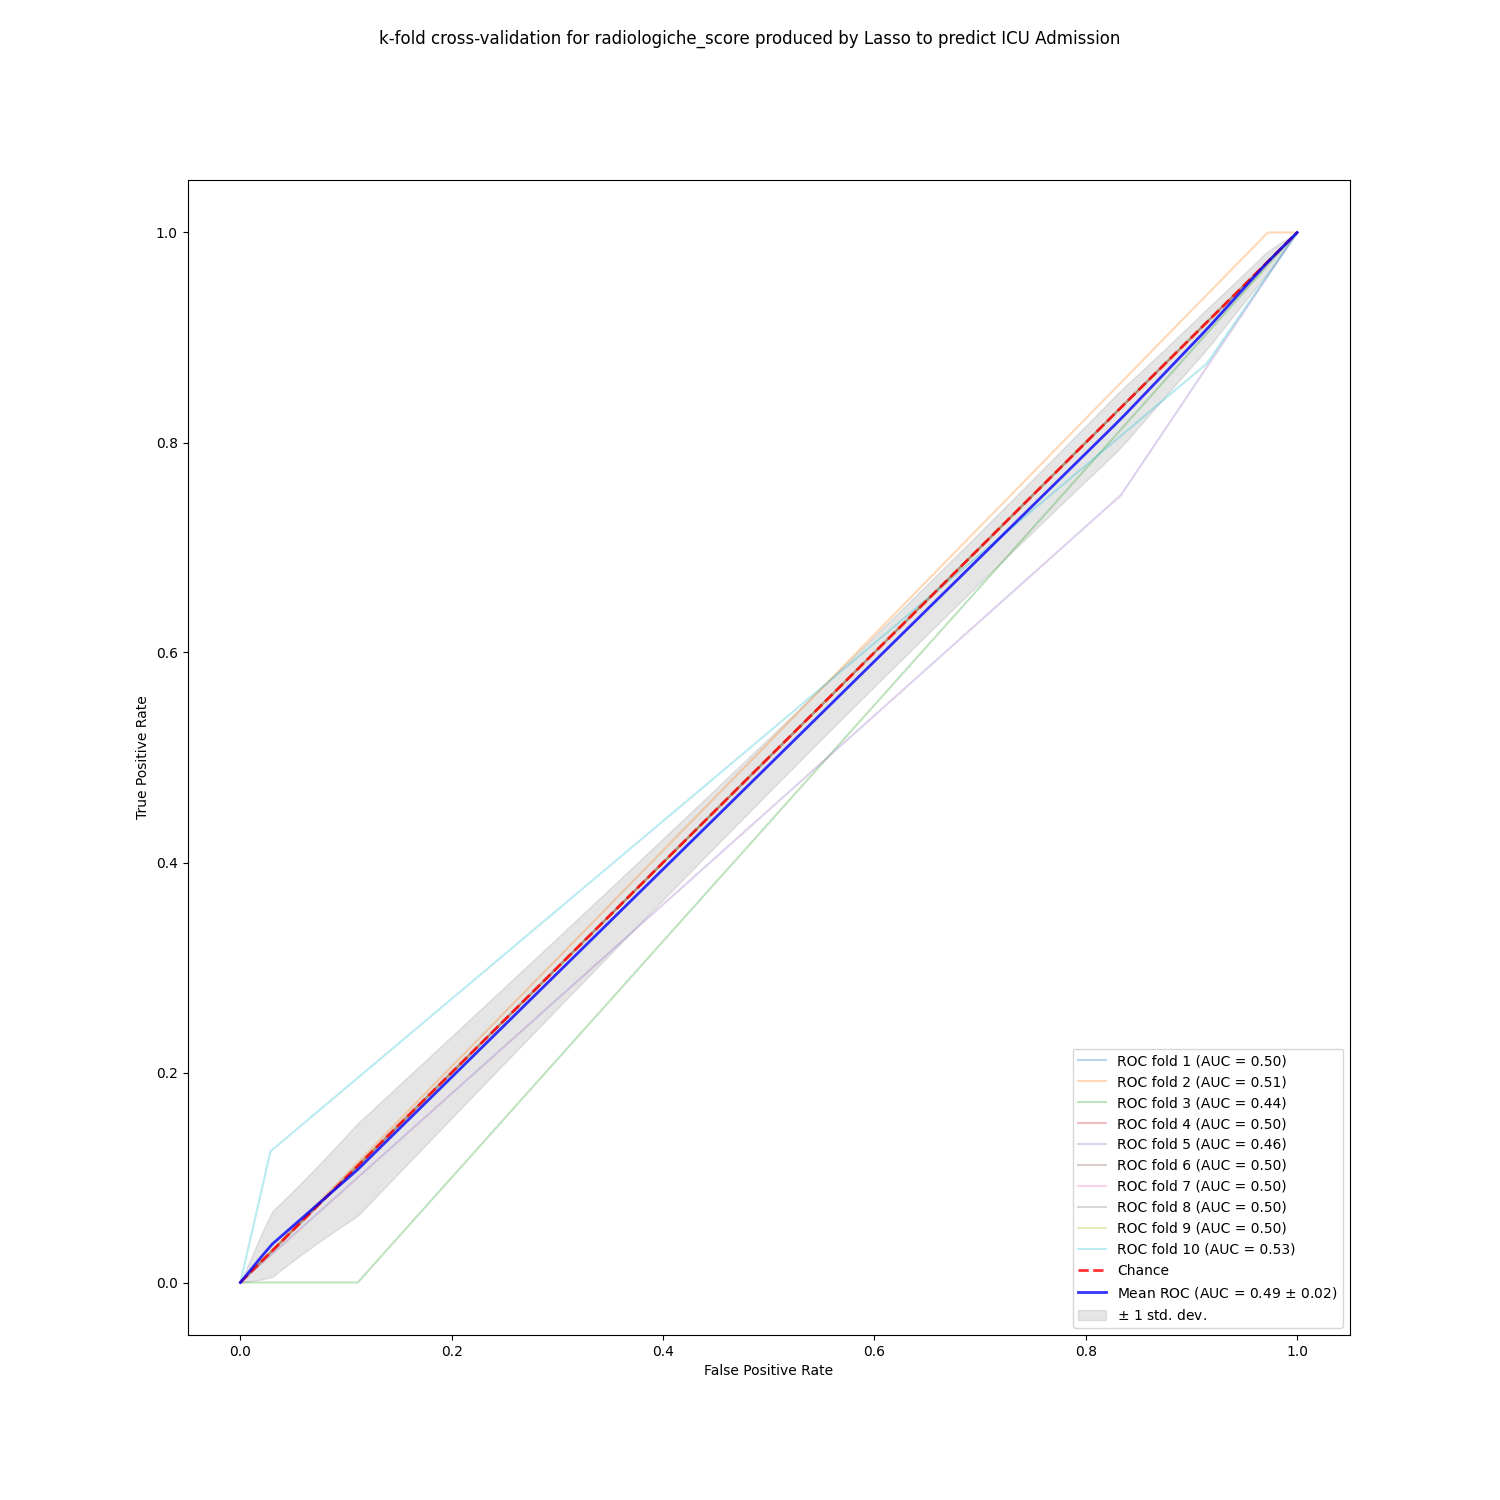
\includegraphics[width=0.50\linewidth]{ROC_CV_radiologiche_icu.png}\label{fig:ROCICUradiolocigal}}
        \subfloat[][All Features]{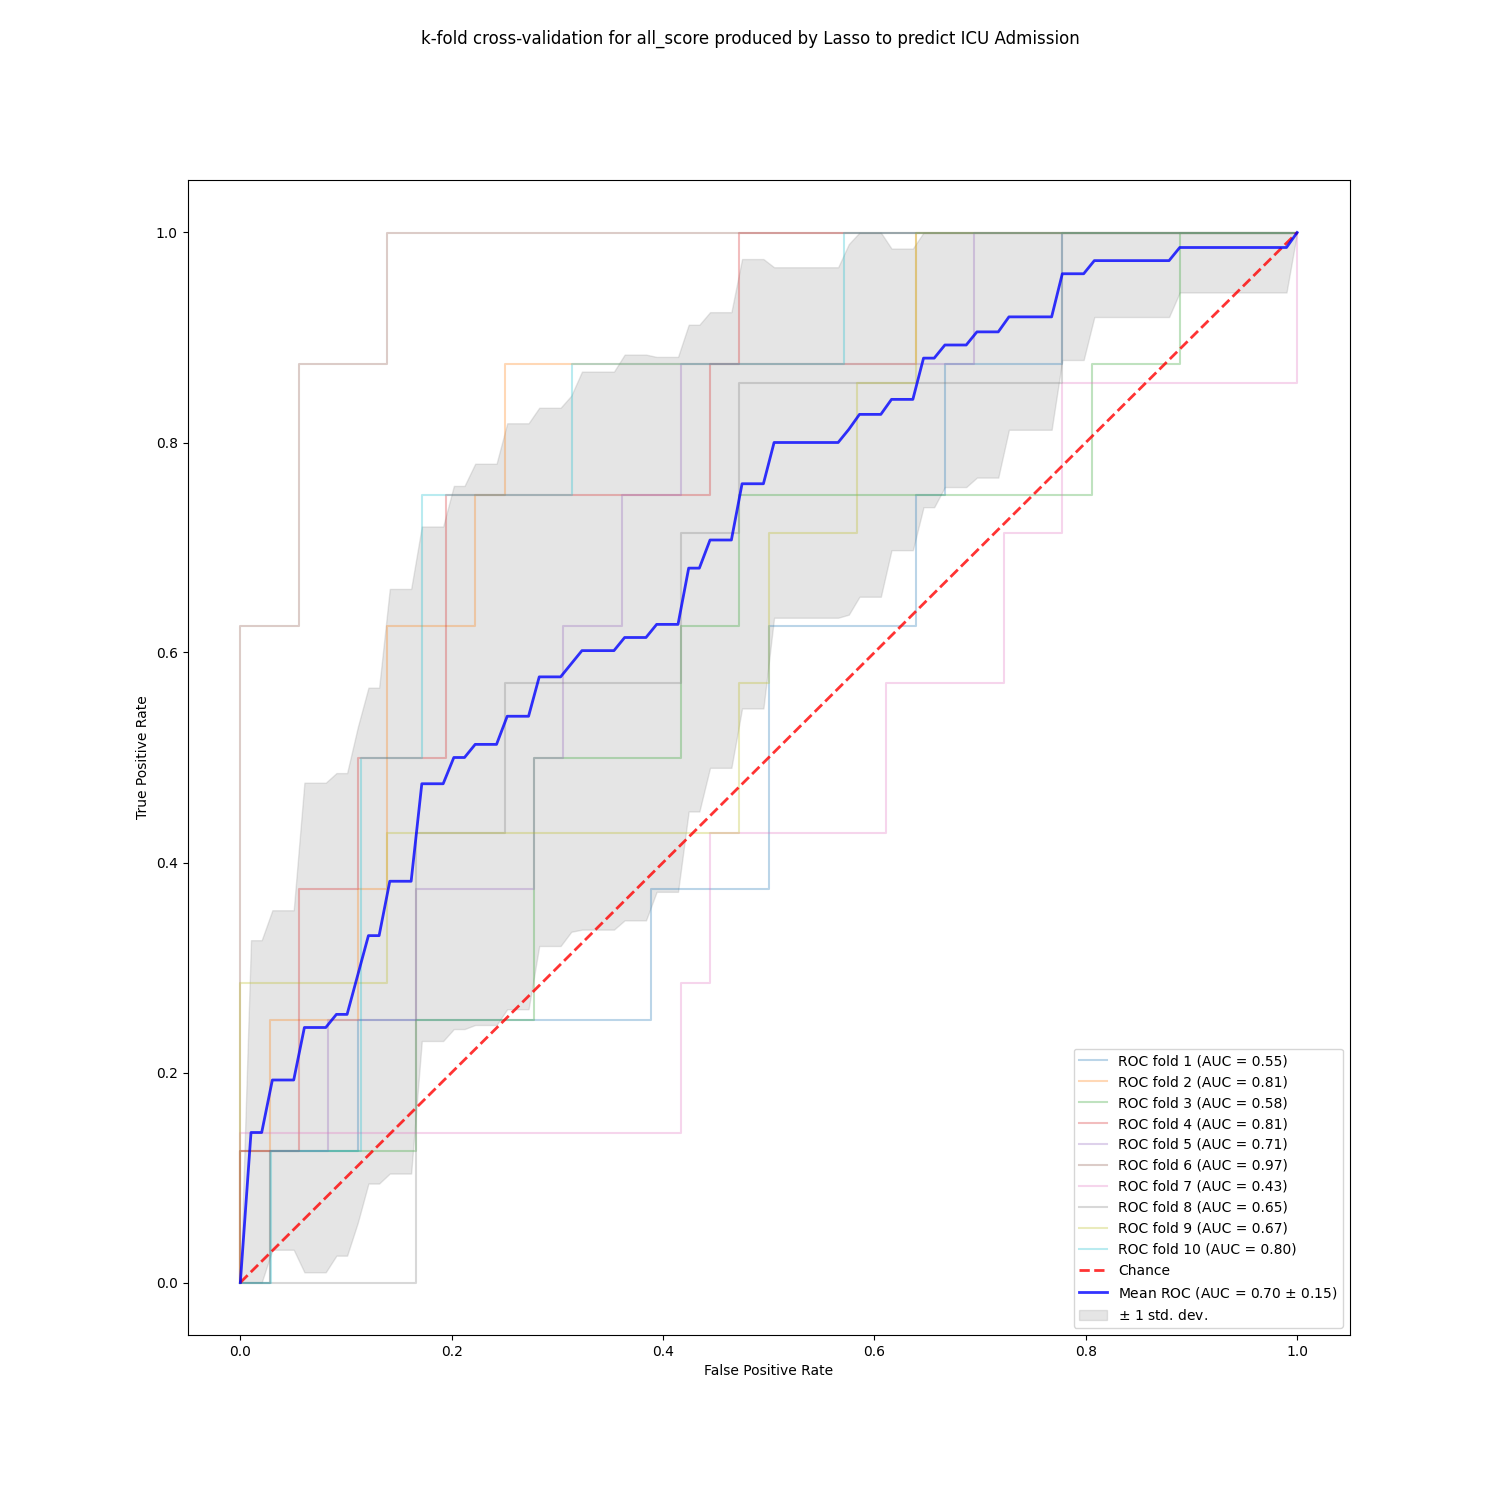
\includegraphics[width=0.50\linewidth]{ROC_CV_all_icu.png}\label{fig:ROCICUall}} 
        \caption{Performances of all the models represented using ROC curves. Each of these has in bold the mean ROC curve over the 10-fold originating from a stratified k-fold cross-validation procedure}\label{fig:ICULasso}
\end{figure}

\begin{table}
\caption{Coefficients used in the linear combination estimated by a Lasso regularization of a model predicting \icu relative to the radiomic features. Values in descending order of modulus \label{tab:ParamRadICU}}
\centering 
	\begin{tabular}{lr}
	\toprule
	Feature Name &   Importance \\
	\midrule
	Intercept                           &                      0.176605 \\
	Number of voxels of positive value  &                      0.160751 \\
	Intensity range                     &                     -0.144834 \\
	Entropy                             &                      0.128999 \\
	Cluster prominence                  &                     -0.122290 \\
	Complexity                          &                     -0.093416 \\
	10th intensity percentile           &                     -0.081133 \\
	Area density - aligned bounding box &                     -0.037373 \\
	Major axis length (cm)              &                     -0.035723 \\
	Dependence count entropy            &                     -0.029603 \\
	Fat.surface                         &                      0.027308 \\
	Asphericity                         &                     -0.023645 \\
	Local intensity peak                &                     -0.019619 \\
	Global intensity peak               &                     -0.016209 \\
	Number of compartments (GMM)        &                     -0.000157 \\
	\bottomrule
	\end{tabular}
\end{table}

\begin{table}
\caption{Coefficients used in the linear combination estimated by a Lasso regularization of a model predicting \icu relative to the clinical features. Values in descending order according to modulus\label{tab:ParamCli}}
\centering
	\begin{tabular}{lr}
	\toprule
	Feature Name &   Importance \\
	\midrule
	Intercept          &                      0.176606 \\
	Respiratory Rate   &                      0.045510 \\
	Febbre             &                      0.038332 \\
	History of smoking &                      0.036888 \\
	Hypertension       &                      0.034547 \\
	Sex\_bin            &                     -0.031504 \\
	Obesity            &                      0.030716 \\
	Age (years)        &                     -0.014646 \\
	\bottomrule
	\end{tabular}
\end{table}


\begin{table}
	\caption{Coefficients used in the linear combination estimated by a Lasso regularization of a model predicting \icu relative to the radiological features\label{tab:ParamRadiologiche}} 
		\centering
			\begin{tabular}{lr}
			\toprule
			Feature Name &   Importance \\
			\midrule
			Intercept             &                  1.766055e-01 \\
			XRayTubeCurrent       &                  0 \\
			Lung consolidation    &                  0\\
			Ground-glass          &                  0\\
			Crazy Paving          &                  0 \\
			Bilateral Involvement &                  0 \\
			SliceThickness        &                 0\\
			KVP                   &                  0 \\
			\bottomrule
			\end{tabular}
\end{table}


\begin{table}
	\caption{Coefficients used in the linear combination estimated by a Lasso regularization of a model predicting \icu relative to all available features features. Values in ascending absolute value order\label{tab:ParamAll}}
		\centering
		\begin{tabular}{lr}
		\toprule
		Feature Name &   Importance \\
		\midrule
		Intercept                           &                      0.176605 \\
		Number of voxels of positive value  &                      0.109947 \\
		Dependence count entropy            &                      0.070527 \\
		Cluster prominence                  &                     -0.069526 \\
		Intensity range                     &                     -0.057924 \\
		Febbre                              &                      0.044149 \\
		Hypertension                        &                      0.039127 \\
		SliceThickness                      &                     -0.037174 \\
		Complexity                          &                     -0.033393 \\
		History of smoking                  &                      0.032812 \\
		Age (years)                         &                     -0.032579 \\
		XRayTubeCurrent                     &                     -0.032182 \\
		Respiratory Rate                    &                      0.028504 \\
		Obesity                             &                      0.027580 \\
		Local intensity peak                &                     -0.026135 \\
		Area density - aligned bounding box &                     -0.023027 \\
		Asphericity                         &                     -0.022999 \\
		Global intensity peak               &                     -0.018280 \\
		Fat.surface                         &                      0.014179 \\
		Sex\_bin                             &                     -0.004316 \\
		Crazy Paving                        &                     -0.003428 \\
		Ground-glass                        &                      0.003077 \\
		Lung consolidation                  &                     -0.001329 \\
		Bilateral Involvement               &                     -0.001047 \\
		Number of compartments (GMM)        &                     -0.000000 \\
		KVP                                 &                      0.000000 \\
		10th intensity percentile           &                     -0.000000 \\
		\bottomrule
		\end{tabular}
\end{table}

Compared to before the performance is definitely worse. 
The radiological features have the same performance of a random variable, which is not that concerning given their expected impact on gravity of the clincial picture of the patient.
Even if superfluous a Delong test was used to confirm that the hypothesis of the curves being equal could not be rejected. When it comes to the relevant features in each model the following can be deduced:

\begin{itemize}
\item For the clinical features all of them have a role in the prediction. The only suprising fact, even if it keeps a certain degree of plausibility, is that age is the less relevant out of the available features when it comes to \icu.
\item None of the radiological features have virtually any impact
\item The radiomic features still value intensity measurements and disorder in the image as primary origins of information. However it seems that shape of the lung now has more relevance in the whole model.
\end{itemize}

\begin{table}
\caption{Recap table with the performance of the various models built for different families of features when predicting \icu \label{tab:RecapICU}}
\centering
\begin{tabular}{l|r}
\toprule
Features used & mean AUC $\pm$std\\
\midrule
Radiomic  & 0.69 $\pm$ 0.13\\
Clinical  &  0.67 $\pm$ 0.14\\
Radiological & 0.49 $\pm$ 0.02\\
All & 0.70 $\pm$ 0.15 \\
\bottomrule
\end{tabular}
\end{table}

\subsection{Classification of patients using Random forests}
Even when using the admission in the ICU the performance of random forests remains pretty much the same when compared to the outcome \death, so the comments would still be the same as before.

\begin{figure}[H]
\centering
  	\subfloat[][Radiomic Features]{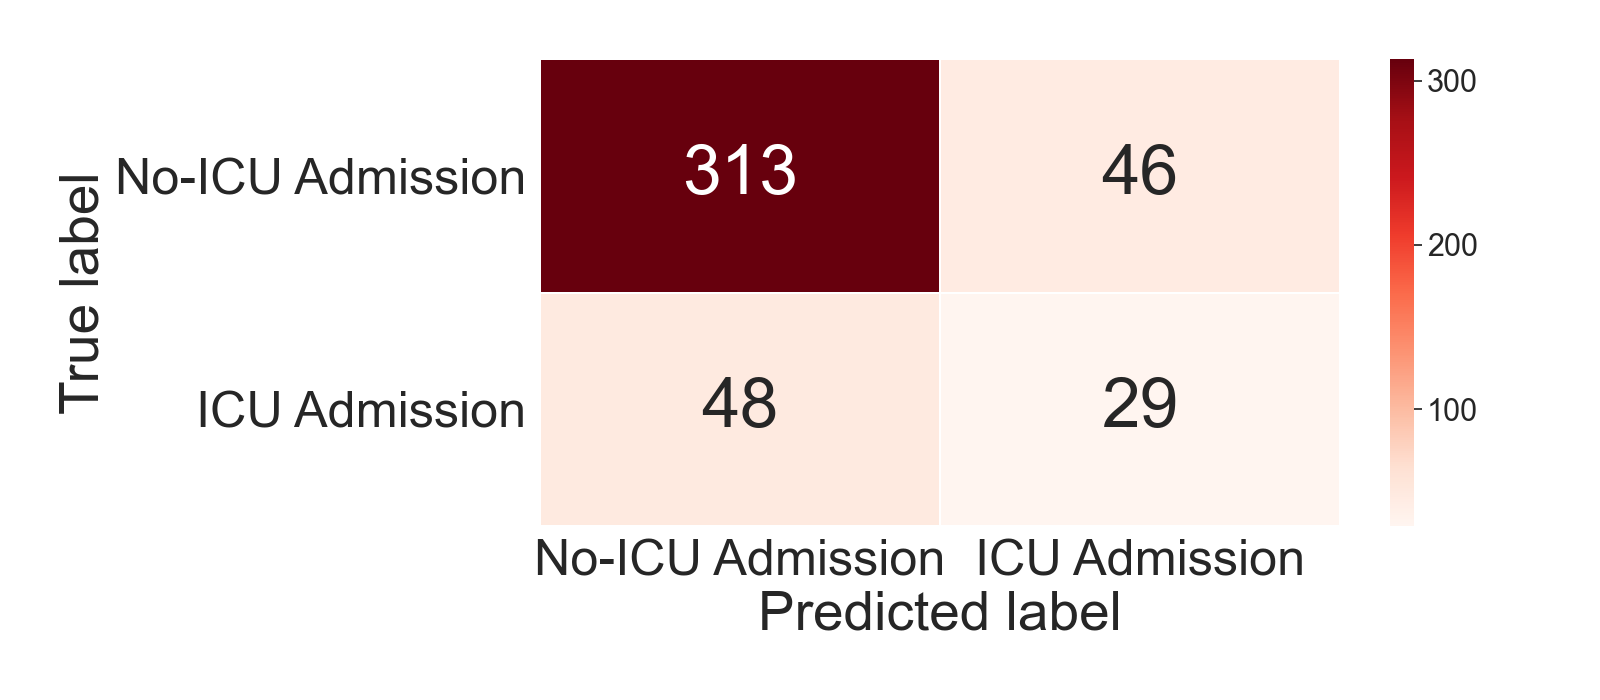
\includegraphics[width=0.50\linewidth]{Smote_ICUAdmission_rad.png}\label{fig:RFicuRad}}
        \subfloat[][Clinical Features]{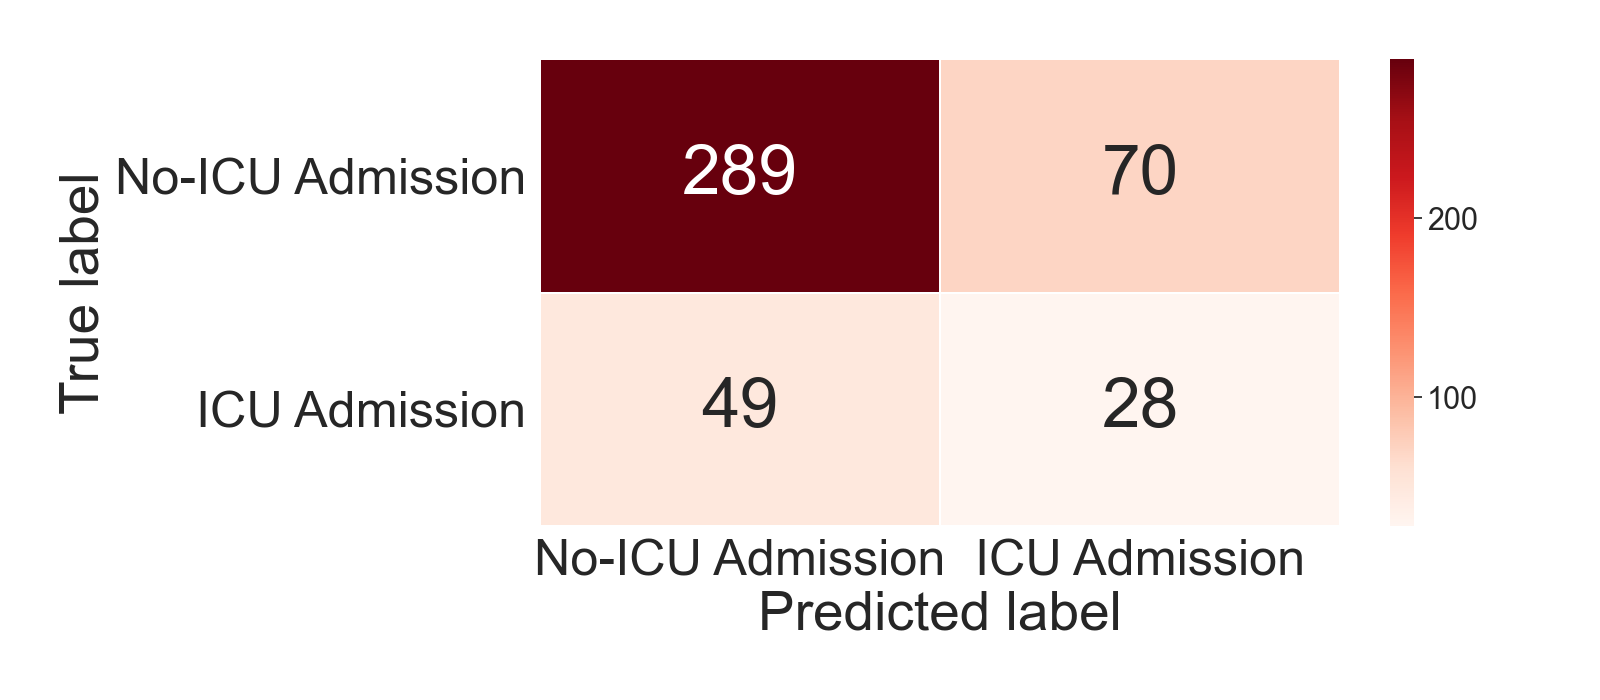
\includegraphics[width=0.50\linewidth]{Smote_ICUAdmission_cli.png}\label{fig:RFicuCli}}
	\newline
  	\subfloat[][Radiological Features]{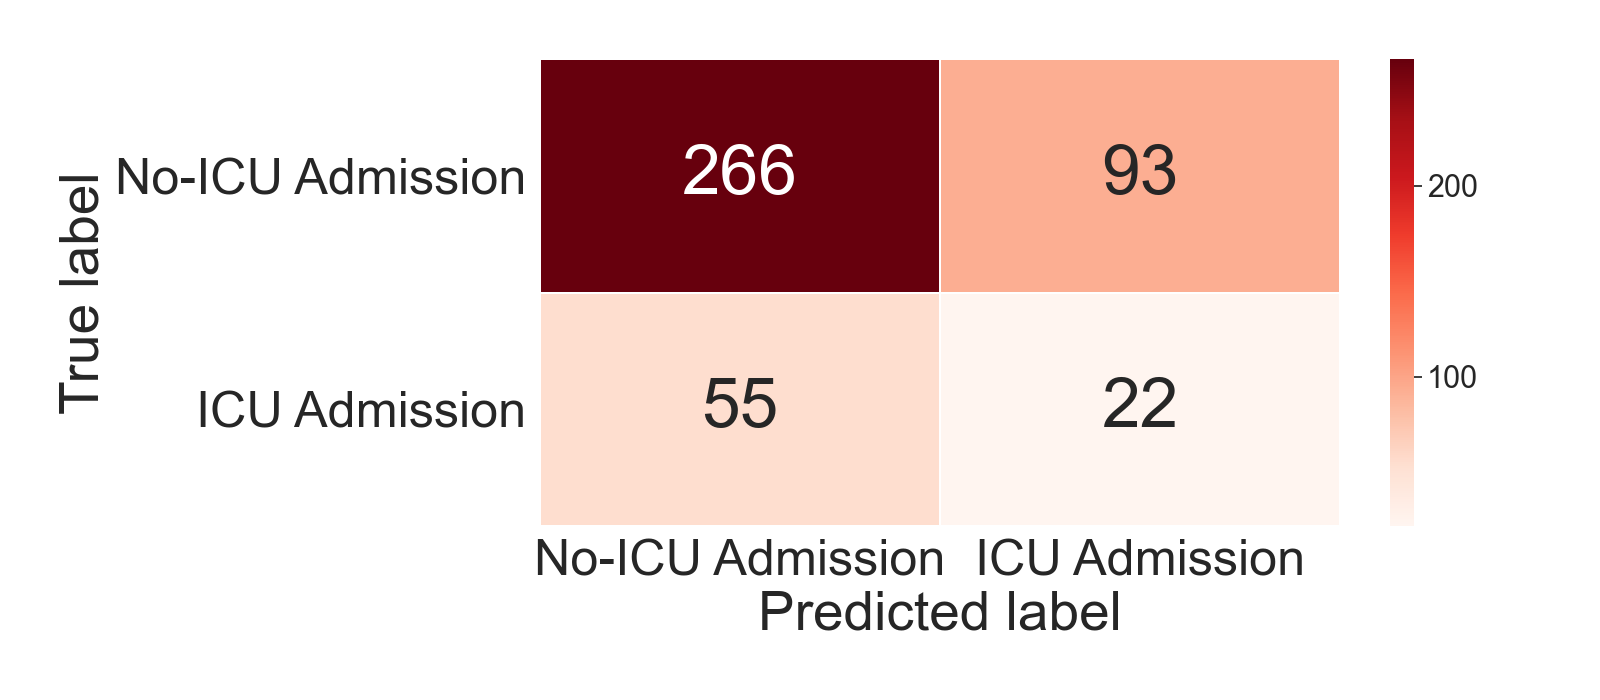
\includegraphics[width=0.50\linewidth]{Smote_ICUAdmission_radiologiche.png}\label{fig:RFicuRadiological}}
        \subfloat[][All Features]{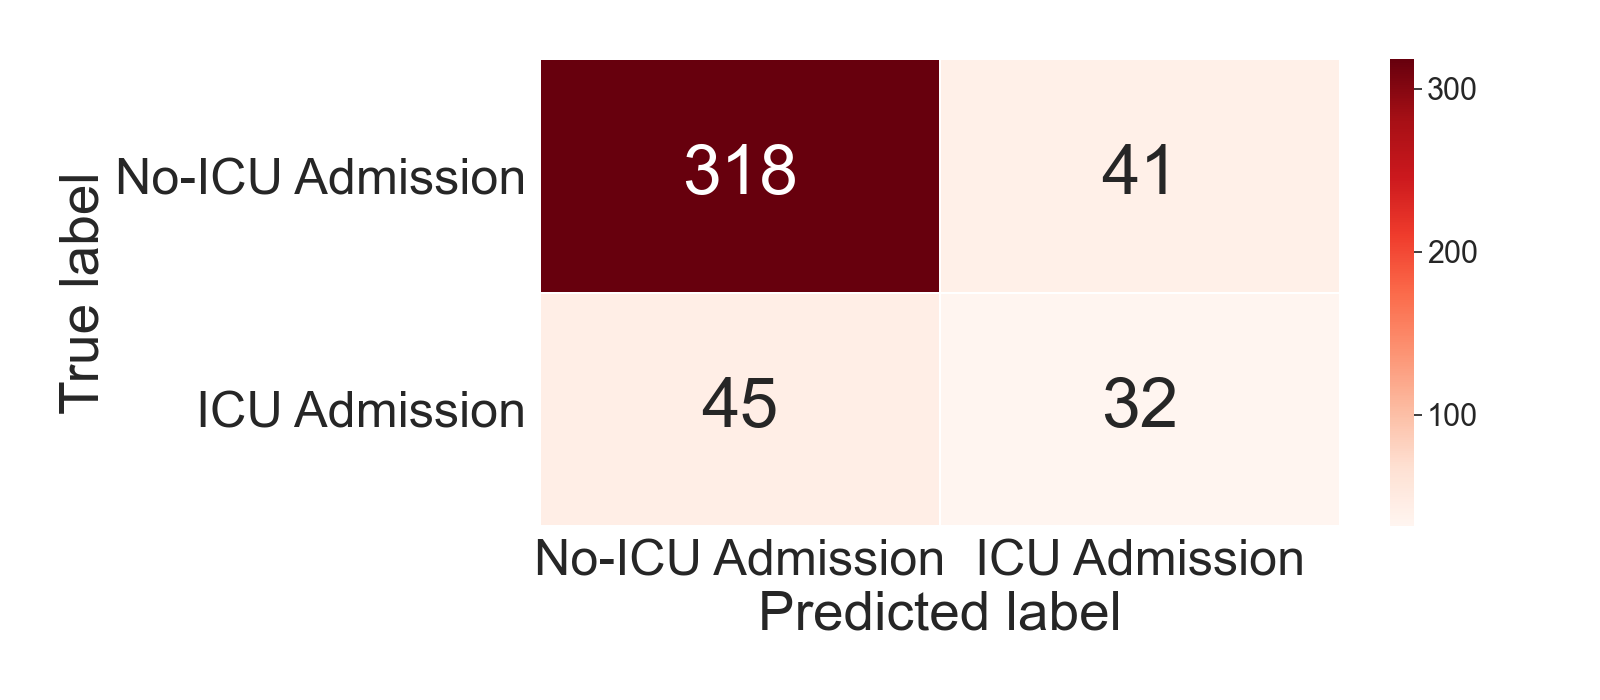
\includegraphics[width=0.50\linewidth]{Smote_ICUAdmission_all.png}\label{fig:RFicuAll}} 
        \caption{Confusion matrices for Random Forest cross-validated predictions after training on Synthetically oversampled data predicting \icu. All of the available feature families are the reported}\label{fig:RFicu}
\end{figure}


\begin{figure}[H]
\centering
  	\subfloat[][Radiomic Features]{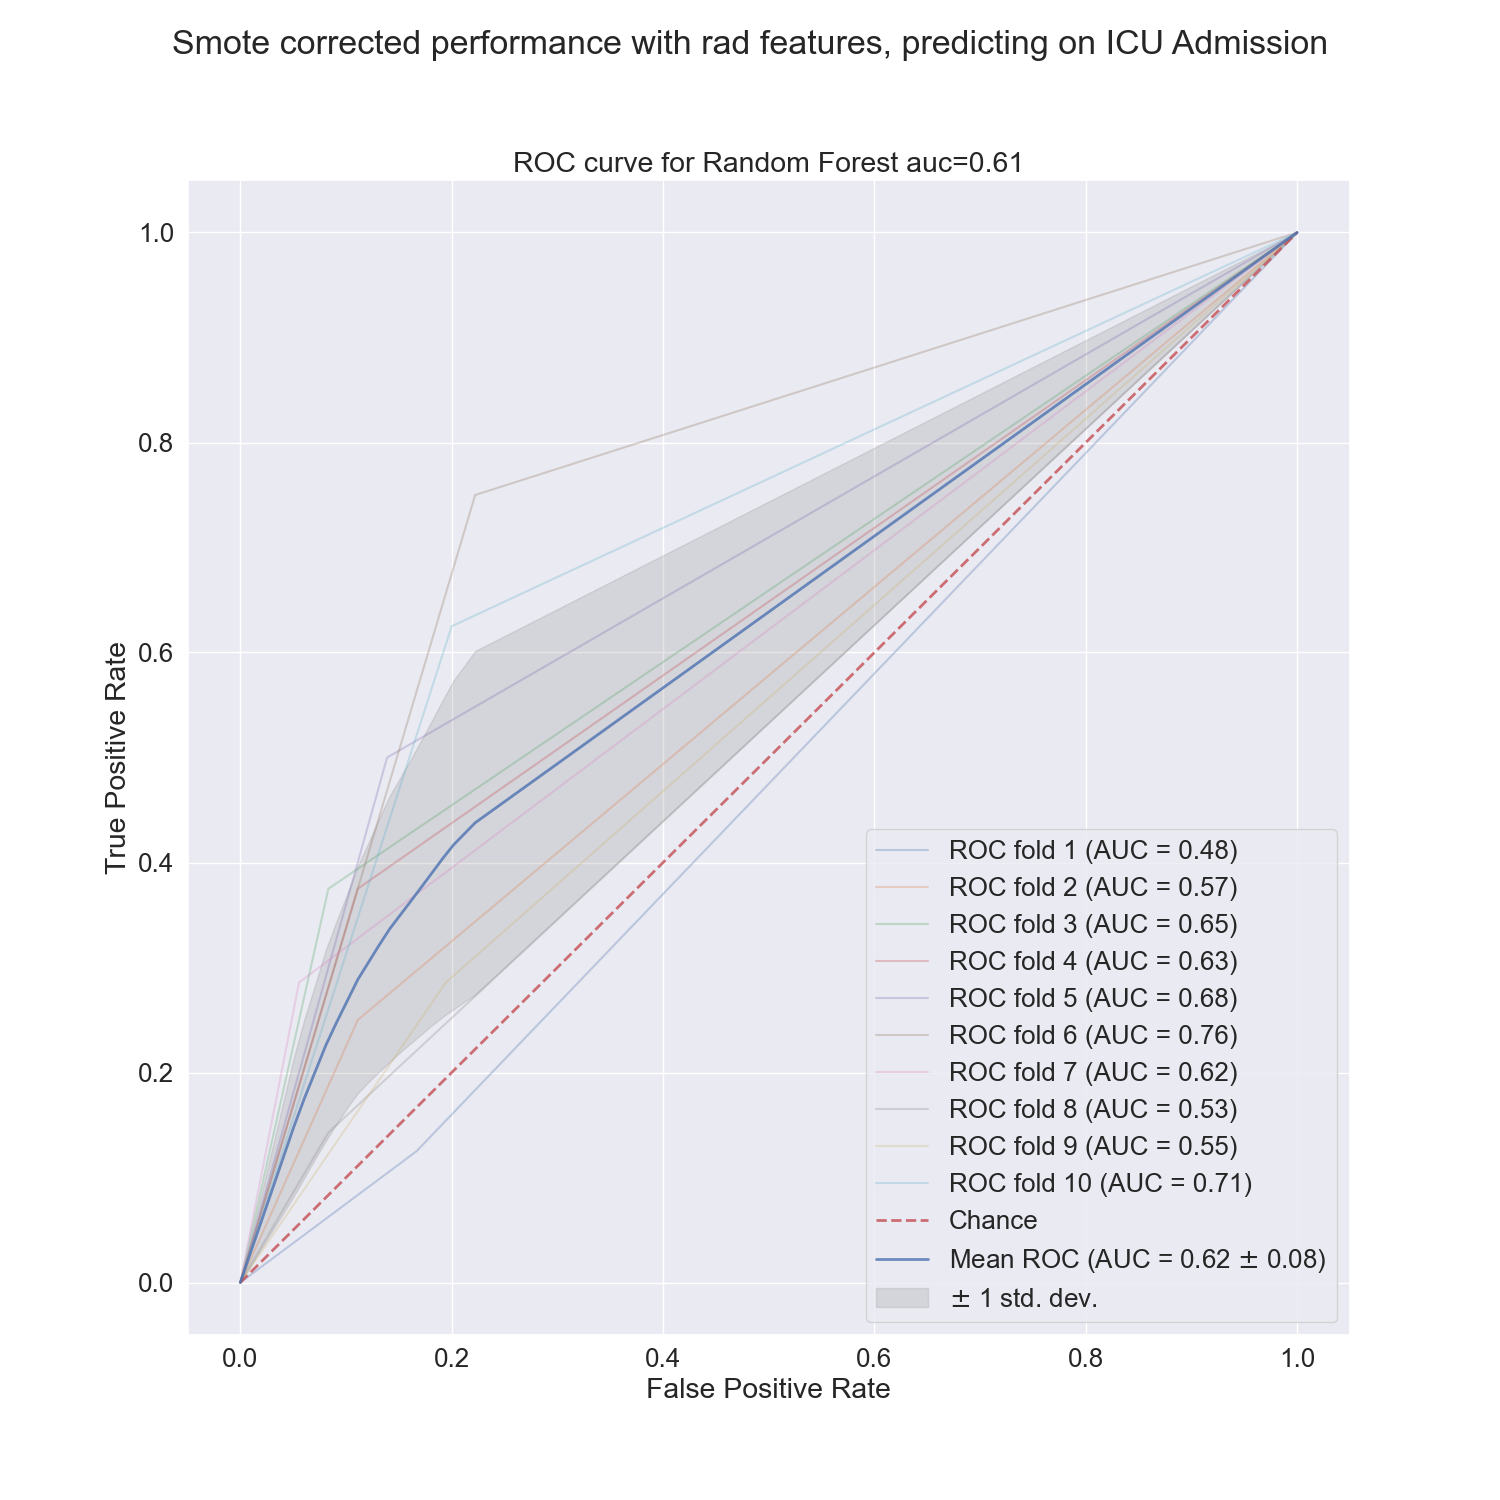
\includegraphics[width=0.50\linewidth]{SmoteROC_CV_ICUAdmission_rad.png}\label{fig:RFicuRadROC}}
        \subfloat[][Clinical Features]{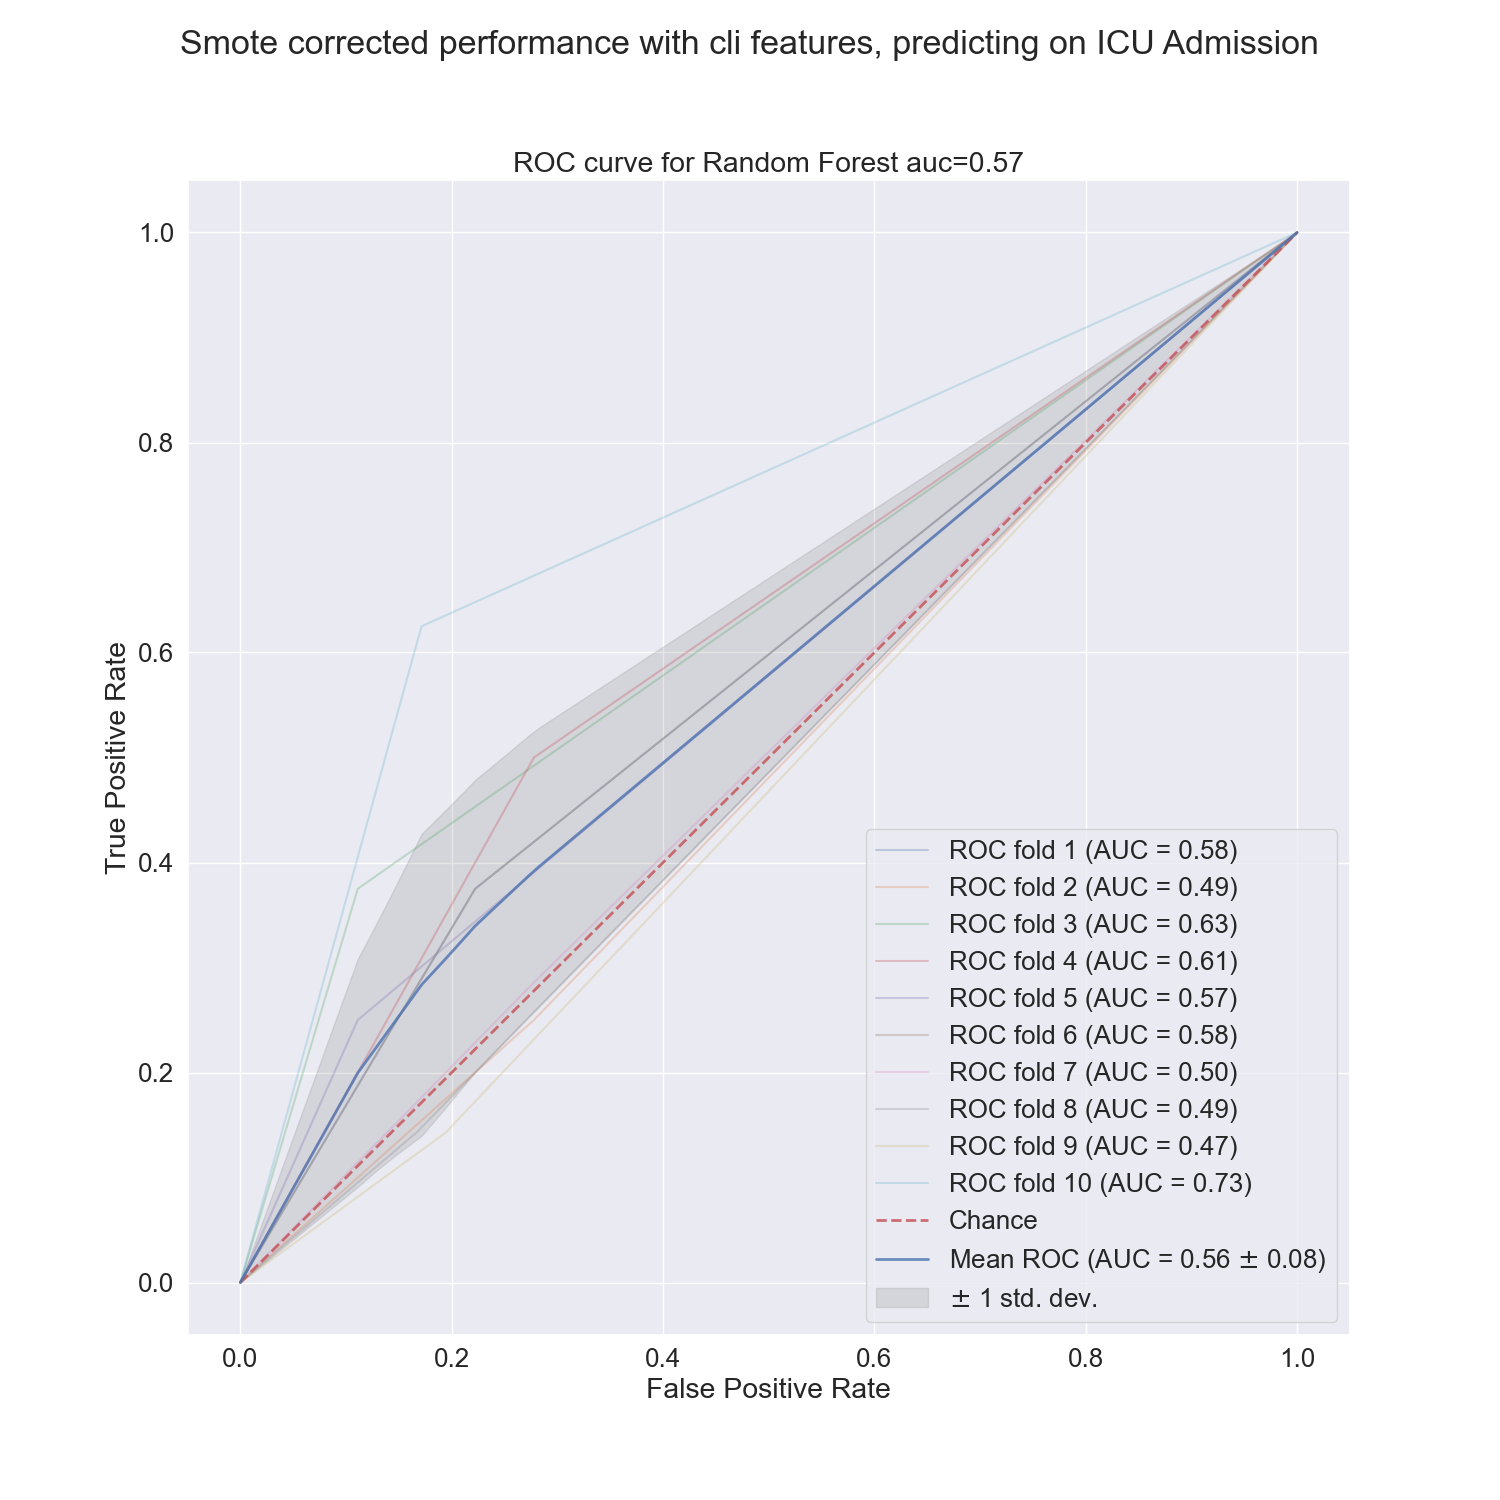
\includegraphics[width=0.50\linewidth]{SmoteROC_CV_ICUAdmission_cli.png}\label{fig:RFicuCliROC}}
	\newline
  	\subfloat[][Radiological Features]{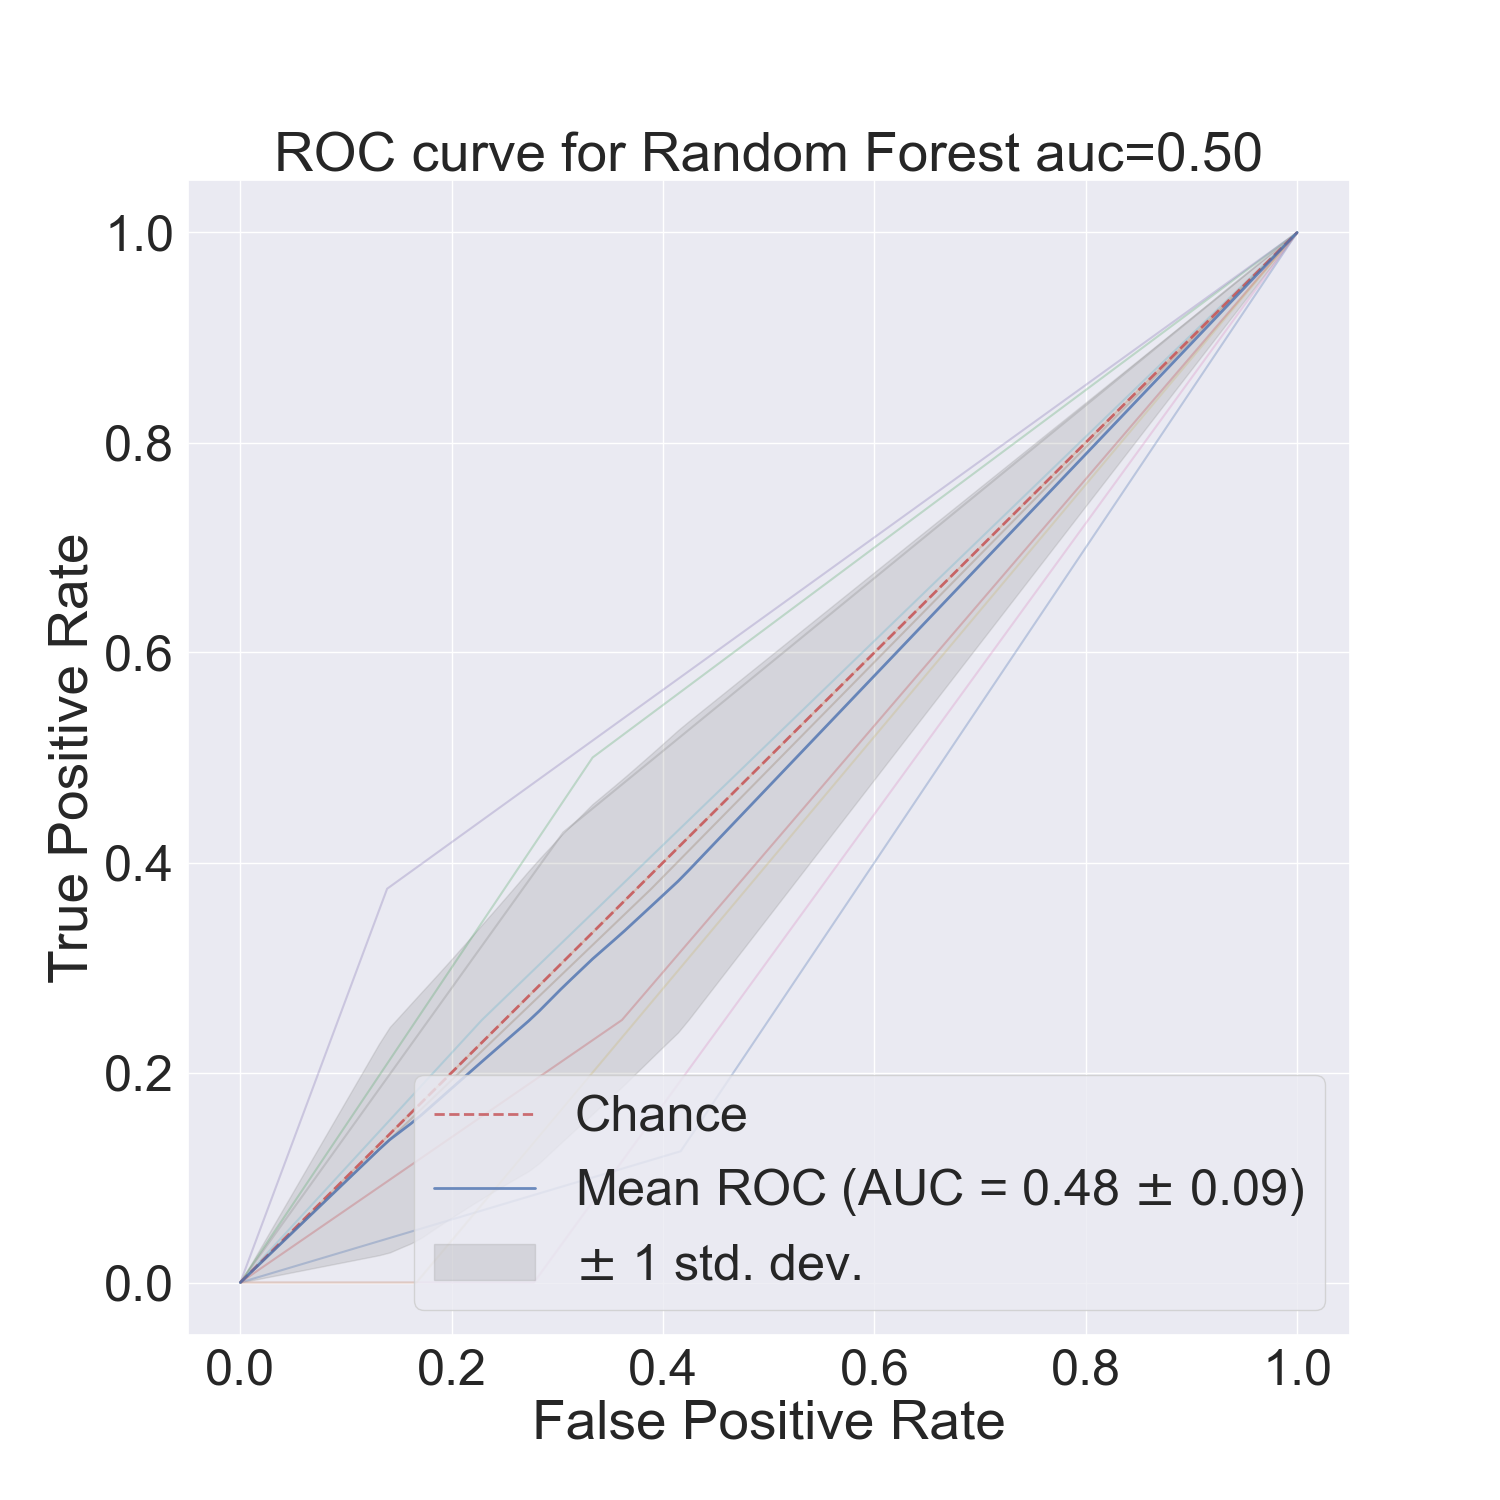
\includegraphics[width=0.50\linewidth]{SmoteROC_CV_ICUAdmission_radiologiche.png}\label{fig:RFicuRadiologicalROC}}
        \subfloat[][All Features]{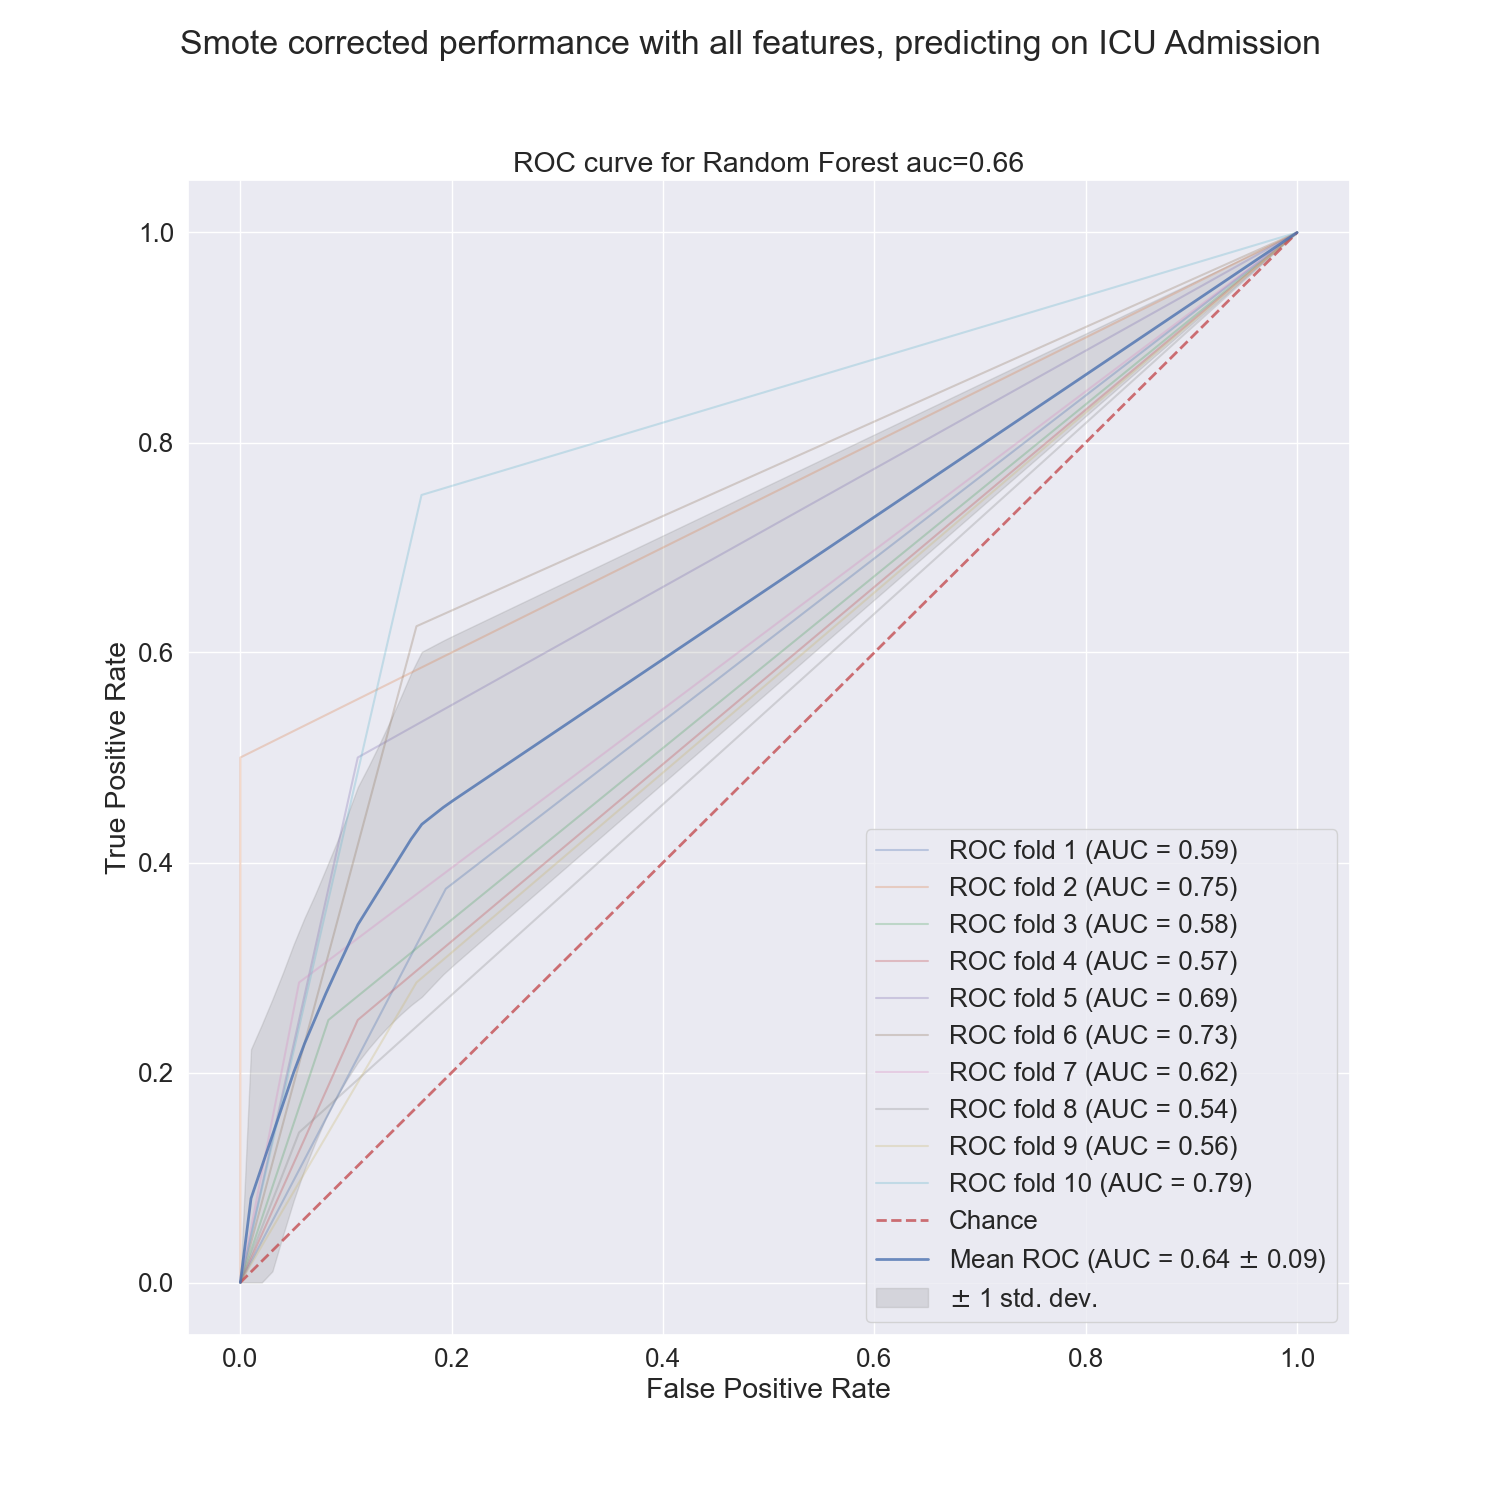
\includegraphics[width=0.50\linewidth]{SmoteROC_CV_ICUAdmission_all.png}\label{fig:RFicuAllROC}} 
        \caption{Cross-validated ROC curves built with Random forest classifier predictions of \death. Performances of allvariable families are reported}\label{fig:RFicuROC}
\end{figure}


\begin{table}
\caption{Recap table with the performance of the various families of features \label{tab:RecapicuRF}}
\centering
\begin{tabular}{l|r}
\toprule
Features used & mean AUC $\pm$std\\
\midrule
Radiomic  & 0.62 $\pm$ 0.08\\
Clinical  &  0.56 $\pm$ 0.08\\
Radiological & 0.51 $\pm$ 0.11\\
All & 0.64 $\pm$ 0.09\\
\bottomrule
\end{tabular}
\end{table}

\section{Using survival analysis}
Following the preprocessing steps delineated in Materials and Methodologies,  a Cox Proportional-Hazard produces the results presented in Table \ref{tab:CoxResult}.

\begin{table}
\centering
\caption{Results obtained with CoxPH fitter from lifelines library\label{tab:CoxResult}}
\begin{adjustbox}{width=\linewidth}
\begin{tabular}{|lrrrrr|}
\toprule
{} &      coef &  exp(coef) &  se(coef) &           p &  -log2(p) \\
covariate                               &           &            &           &                 &               \\
\midrule
Lung consolidation                     			&  0.166411 &   1.181058 &  0.142506 &        0.242908 &  2.041517 \\
Ground-glass                            			&  0.100946 &   1.106217 &  0.134109 &        0.451619 &  1.146822 \\
Crazy Paving                             			&  0.064744 &   1.066886 &  0.140817 &        0.645680 &  0.631108 \\
Bilateral Involvement                  			& -0.026048 &   0.974288 &  0.121990 &        0.830918 &  0.267222 \\
SliceThickness                          			& -0.008439 &   0.991597 &  0.164518 &        0.959092 &  0.060259 \\
KVP                                        			&  0.376184 &   1.456715 &  0.139983 &        0.007202 &  7.117333 \\
XRayTubeCurrent                     			& -0.272076 &   0.761796 &  0.178915 &        0.128335 &  2.962010 \\
Age (years)                              			& -0.016550 &   0.983587 &  0.160470 &        0.917858 &  0.123657 \\
Hypertension                            			&  0.292450 &   1.339705 &  0.160211 &        0.067940 &  3.879603 \\
History of smoking                    			& -0.083840 &   0.919578 &  0.139121 &         0.546747 &  0.871054 \\
Obesity                                    			&  0.066777 &   1.069057 &  0.170581 &         0.695451 &  0.523979 \\
Respiratory Rate                      			& -0.010716 &   0.989341 &  0.154003 &         0.944525 &  0.082338 \\
Sex\_bin                                 			& -0.366086 &   0.693443 &  0.172651 &         0.033974 &  4.879413 \\
Febbre                                     		  	&  0.115458 &   1.122387 &  0.139878 &         0.409134 &  1.289354 \\
10th intensity percentile             			&  0.324188 &   1.382908 &  0.230611 &        0.159790 &  2.645753 \\
Area density - aligned bounding box     	& -0.169228 &   0.844316 &  0.185602 &        0.361884 &  1.466401 \\
Asphericity                             			& -0.470777 &   0.624517 &  0.174449 &         0.006962 &  7.166236 \\
Cluster prominence                      		& -0.011242 &   0.988821 &  0.234222 &        0.961720 &  0.056312 \\
Complexity                              			&  0.214330 &   1.239032 &  0.248380 &         0.388186 &  1.365179 \\
Global intensity peak                   		&  0.138264 &   1.148279 &  0.165033 &         0.402146 &  1.314210 \\
Intensity range                        			& -0.196751 &   0.821395 &  0.281701 &        0.484901 &  1.044237 \\
Local intensity peak                    			&  0.132819 &   1.142044 &  0.150161 &        0.376419 &  1.409589 \\
Number of compartments (GMM)            	&  0.197884 &   1.218821 &  0.140554 &         0.159164 &  2.651410 \\
Number of voxels of positive value      		&  0.436757 &   1.547680 &  0.284518 &         0.124764 &  3.002721 \\
Fat.surface                             			& -0.425033 &   0.653748 &  0.208060 &        0.041069 &  4.605815 \\
Normalised zone distance non-uniformity 	&  0.589917 &   1.803838 &  0.242437 &         0.014963 &  6.062489 \\
\bottomrule
\end{tabular}
\end{adjustbox}
\end{table}

\begin{figure}
\caption{Graph that represents the coefficient values estimated by the CoxPH model with their respective 95\% confidence intervals}
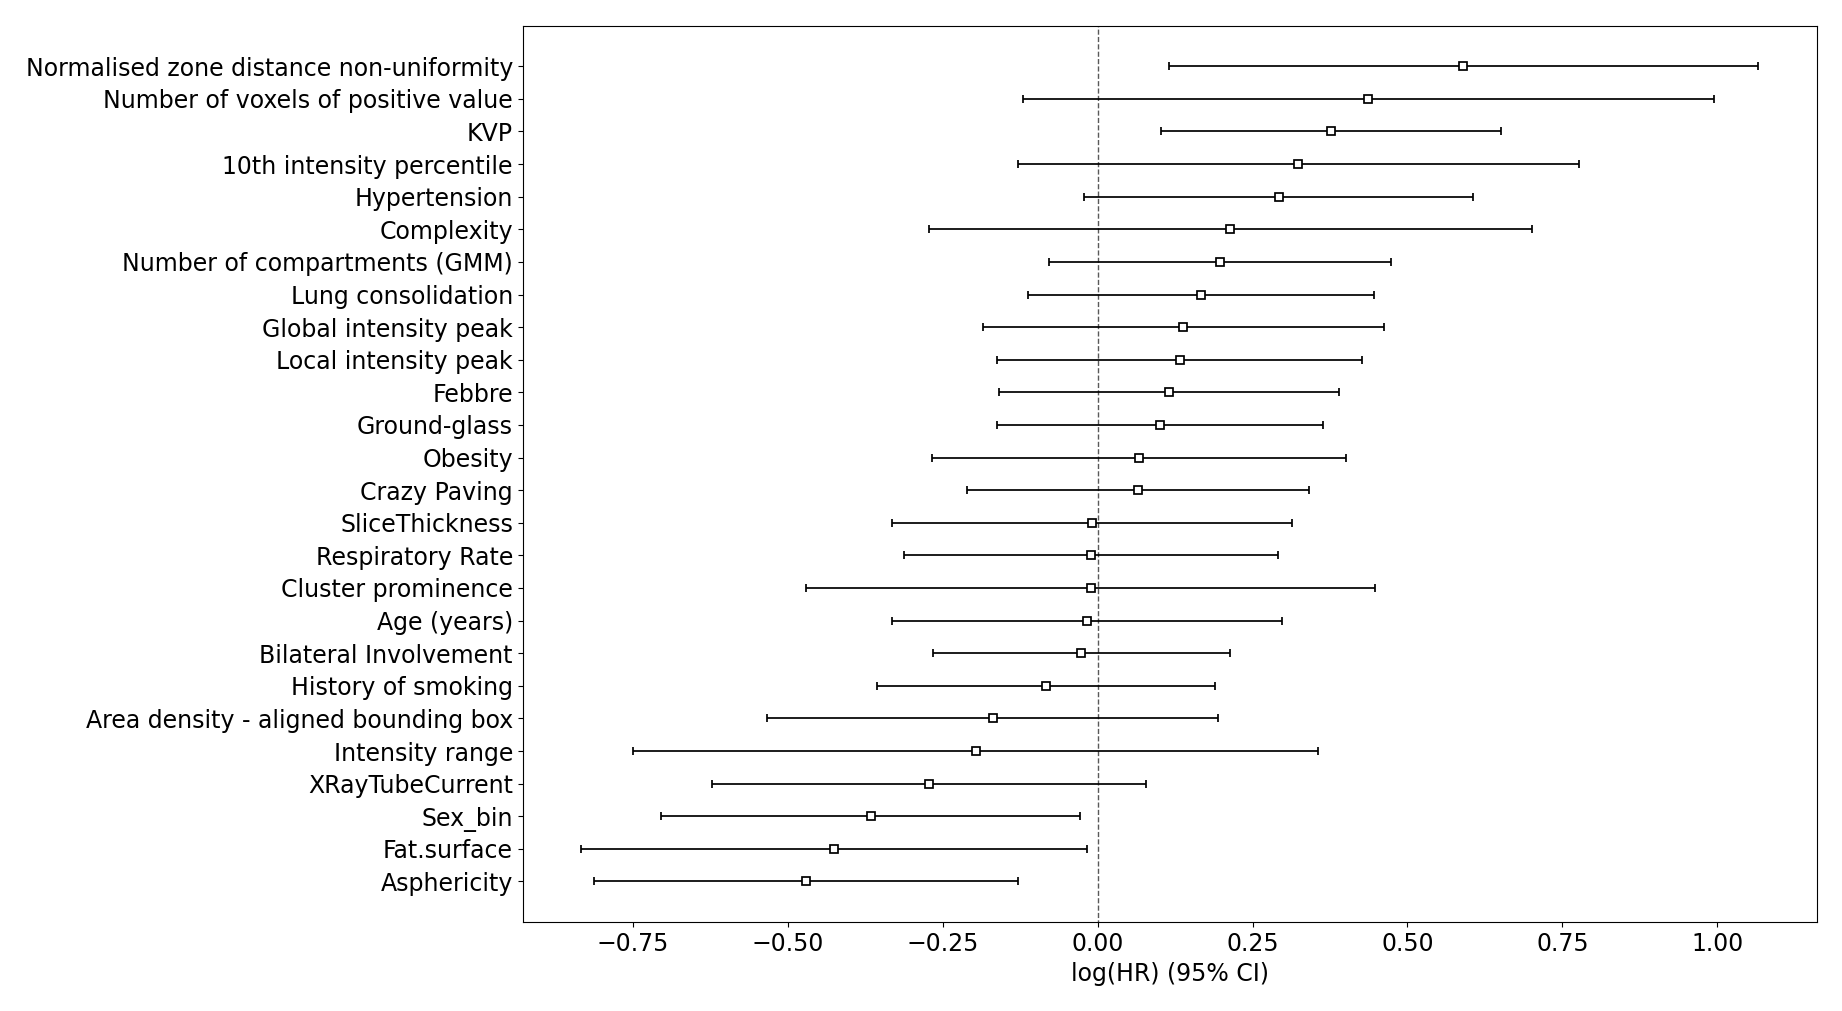
\includegraphics[width=\textwidth]{Cox_coeffs.png}
\end{figure}

As explained in section \ref{sec:SurvivalAnalysisTheory} the relevant columns are the coeff column, that expressed percentual difference of survival, and the p column, that indicate the significance of the first value.
It turns out that, out of the reduced variables fed to the Cox model, the most relevant are: {\scshape Sex, Asphericity, FatSurface, Normalized zone distance non-uniformity and KVP}.

{\scshape Zone distance non uniformity} measures distribution of zone counts over the different zone distances, it is low when the count relative to the zones are equally distributed along zone distances

{\scshape Asphericity} quantifies how much the segmented region deviates from a sphere.


In this case{\scshape Sex} and {\scshape FatSurface} and {\scshape Normalized zone distance non-uniformity} can be reasonable variables to expect, however {\scshape KVP, Asphericity} seem quite strange.

A score was built automatically using the predict method of the CoxPH fitter and assigned to each patient of the dataset using the previously described cross-validated prediction procedure.
To see if the prediction was representative of differences in the individuated populations first the Kaplan-Meier curves according to thirds in the score distribution were used and then the score was binarized using the 66$^{th}$ percentile in the score distribution as threshold.
The results of this procedures are reported in Figure \ref{fig:KmCoxScore}

\begin{figure}[H]
\centering
  	\subfloat[][Population divided according to score tertiles]{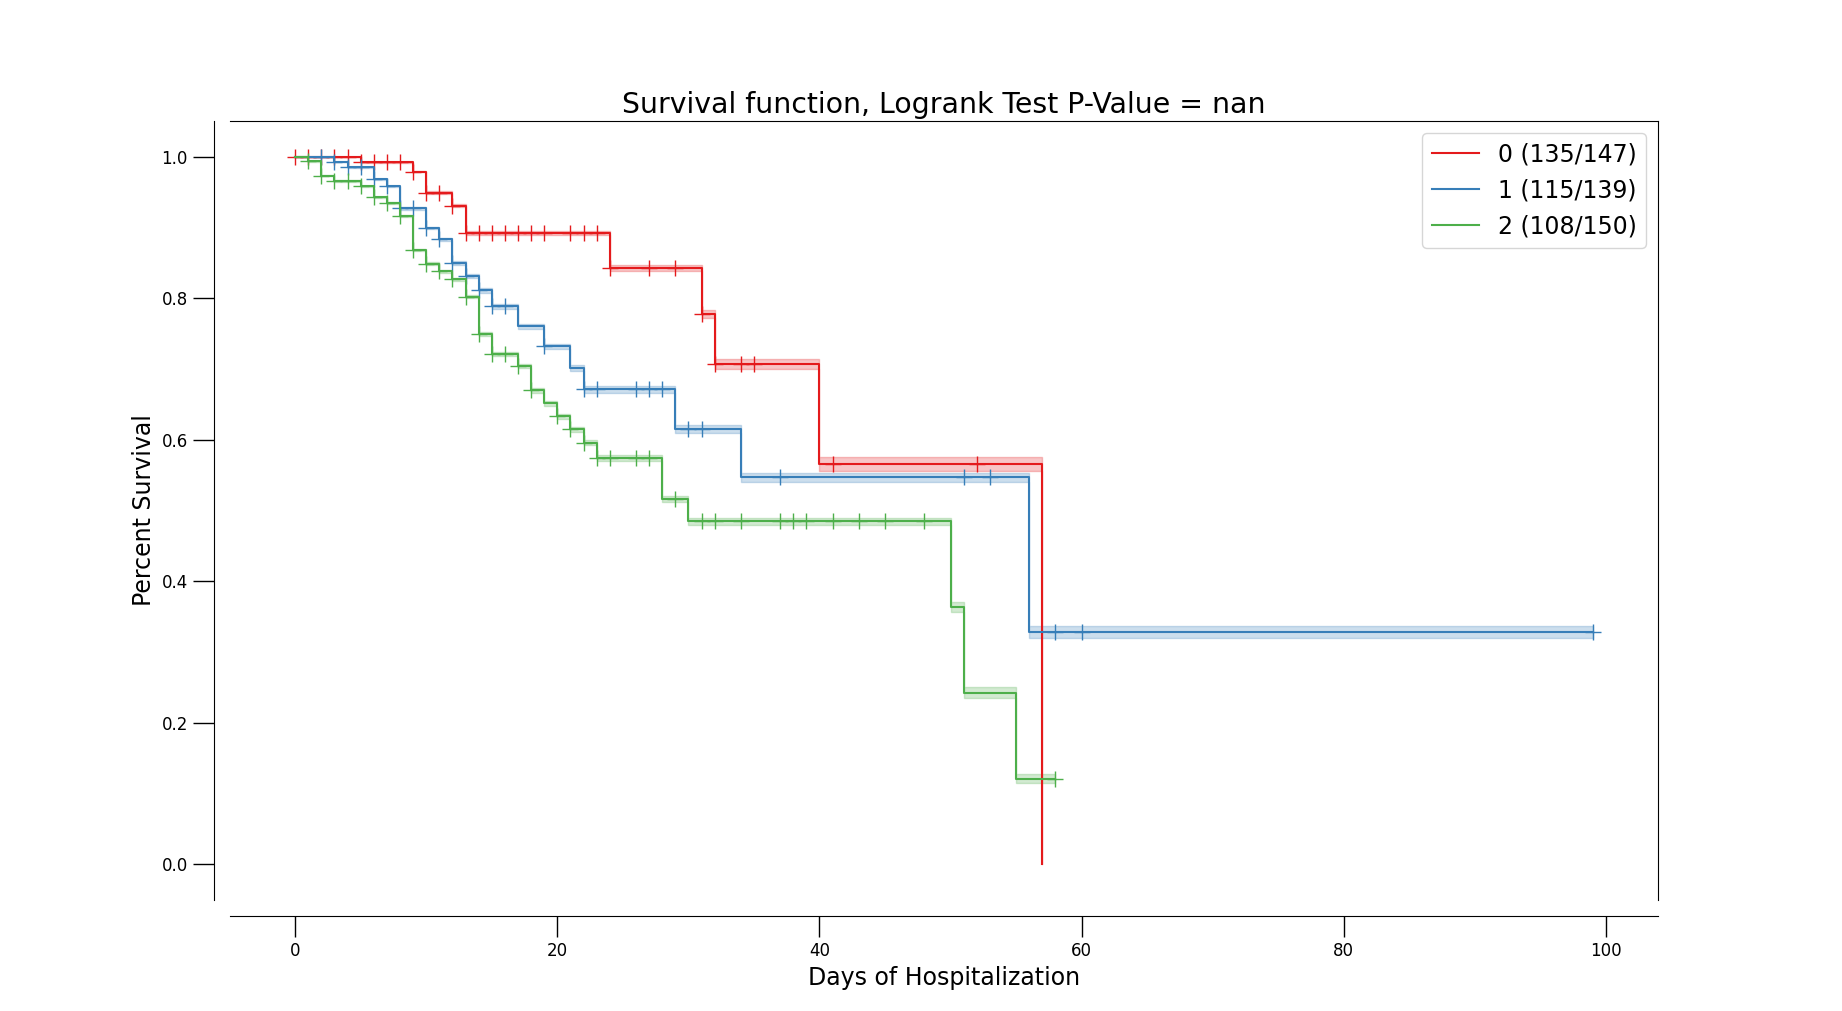
\includegraphics[width=\linewidth]{KM_Cox_groups.png}\label{fig:coxthirds}}
	\newline
        \subfloat[][Population divided in two groups 0-66$^{th}$ percentile and 66$^{th}$ to 100$^{th}$]{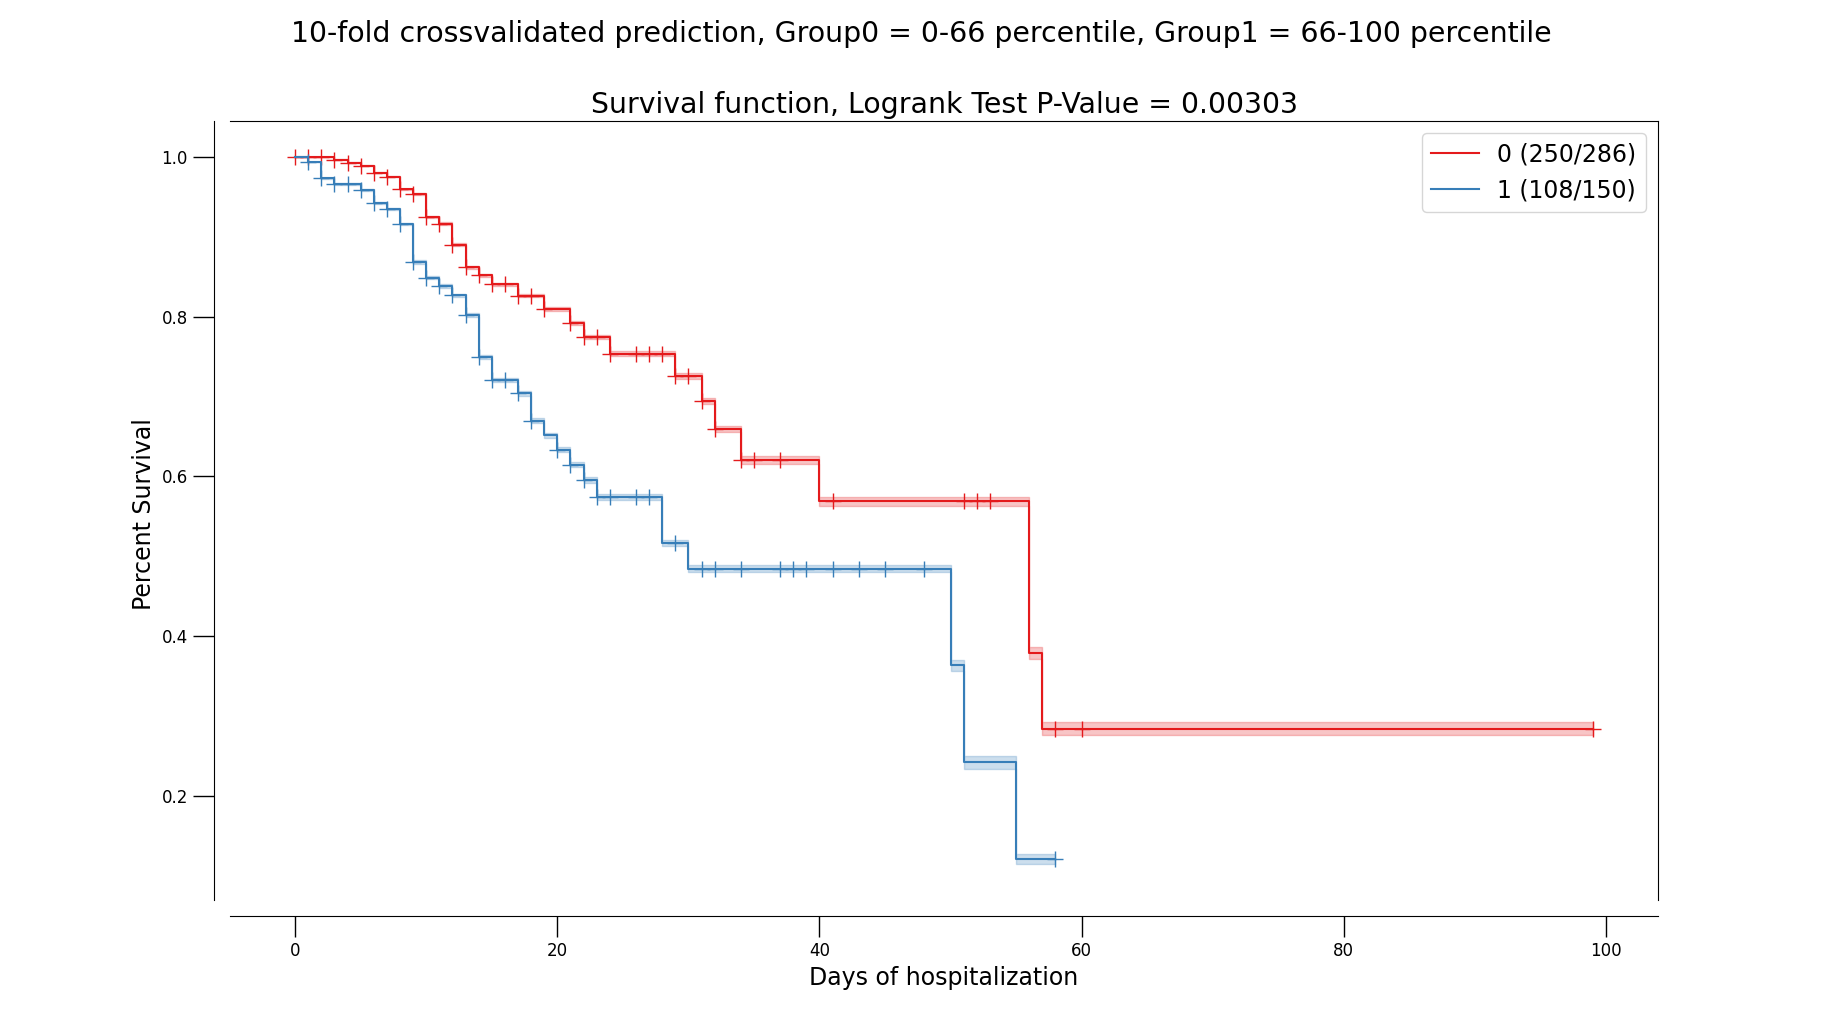
\includegraphics[width=\linewidth]{KM_Coxbin.png}\label{fig:coxbin}}
        \caption{Kaplan-Meier curves for pupulations divided using either tertiles in the predicted hazard by the cox model (a) or binarized using 66$^{th}$ percentile as threshold (b) . The prediction on the whole database is obtained with the aforementioned cross-validation procedure }\label{fig:KmCoxScore}
\end{figure}

It can be seen that the groups built in this ways can be used to drive some differences in survival, when binarizing the score obtained with Cox the curves also turn out to be significantly different.

Finally, in order to see if there were differences in treatment or in survival between the two waves of admission, the population was divided in two subgroups according to the date of admission. 
The two groups were representatively called 1$^{st}$ and 2$^{nd}$ wave and the division was drawn on the 20$^{th}$ of July 2020 and the results can be seen in Figure \ref{fig:kmwaves}.

\begin{figure}
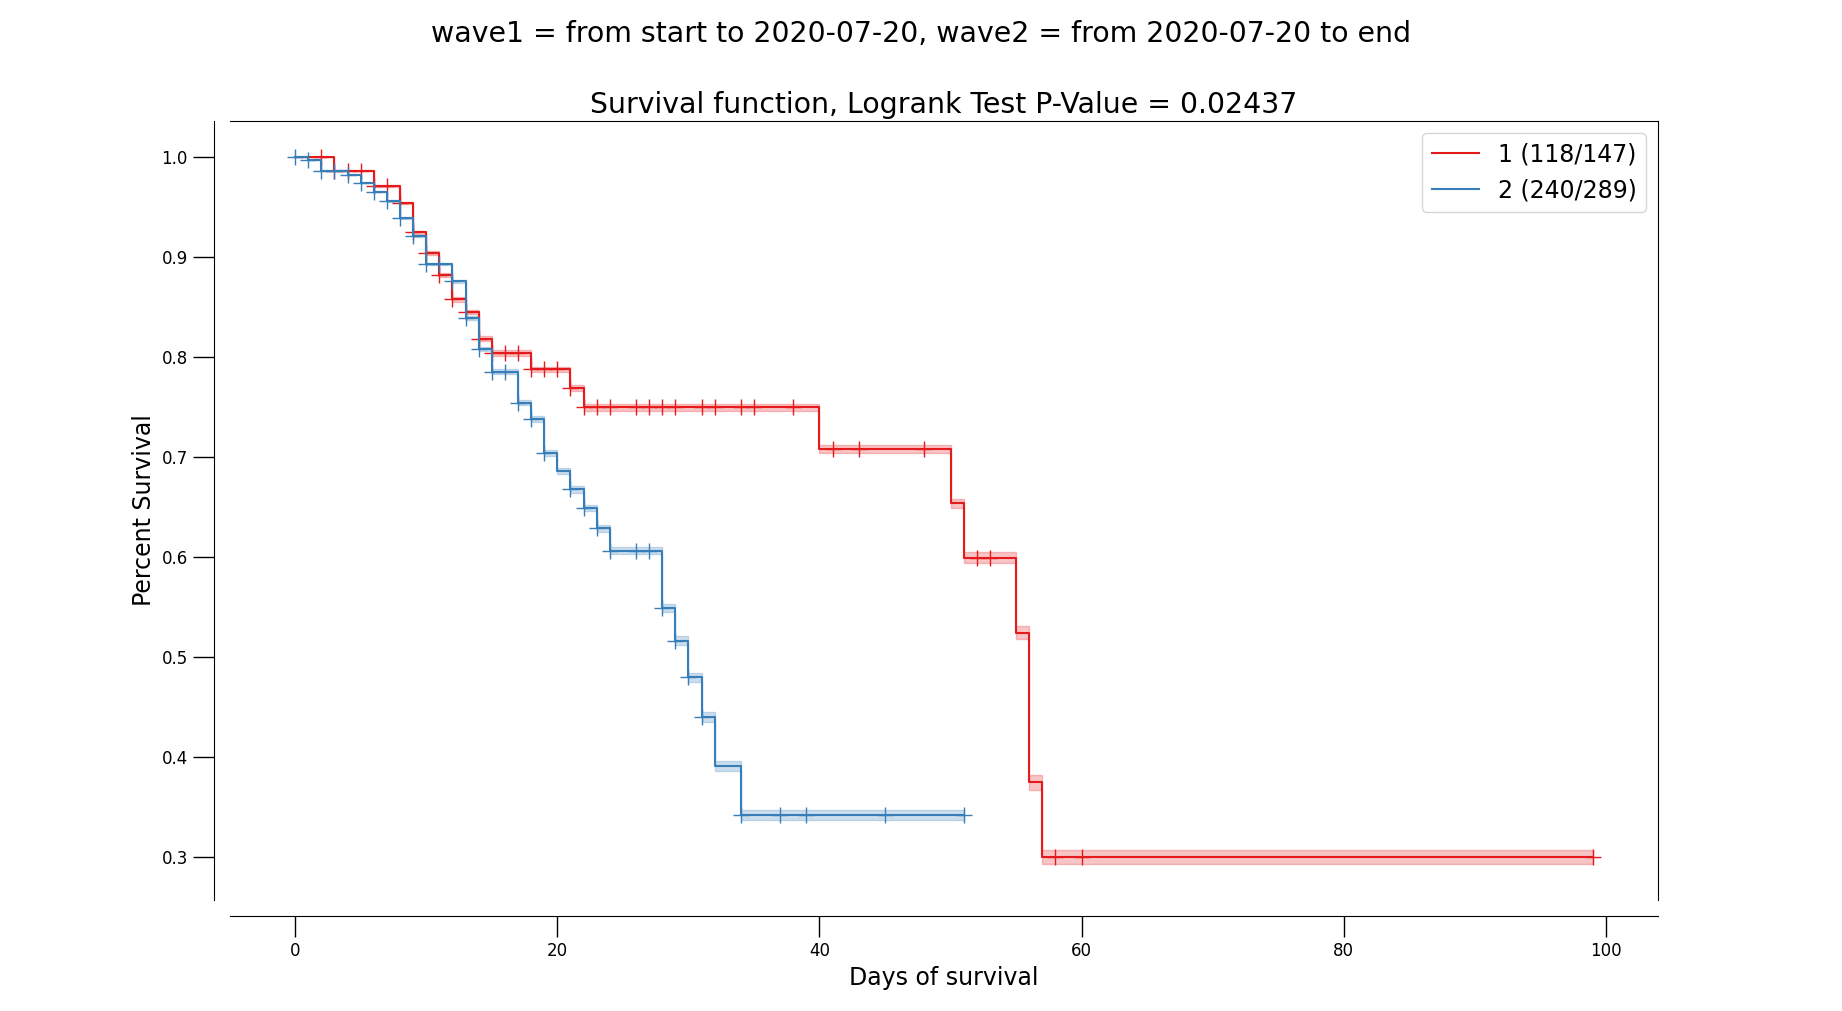
\includegraphics[width=\linewidth]{KM_ondate.png}
\caption{Kaplan-Meyer curves for patient admitted before (red curve) and after (blue curve) 20/07/2020 \label{fig:kmwaves}}
\end{figure}

It can be seen that there is a statistical difference in survival between the patients admitted in the first wave vs those admitted in the second. 
Furthermore this difference is quite perplexing as it seems to indicate that people in the second wave died more than people in the first wave, which seems counter-intuitive given that one would expect the experience from the previous wave to improve performance.
The most reasonable explanation for this fact is the change in admission policy as time advanced.
Probably in the first wave, when still little was known on \covid patients, more people were addmitted in less problematic condition whereas in the second wave, having understood better what were the most dangerous cases as well as in an attempt to admitt only those  strictly in need, most of the admitted patients were in more critical condition.

It's also possible that this result that has been obtained could be a symptom of subtle differences in the two \covid manifestations, as if to indicate different variants.
Further analysis in this direction could be a followup work of this thesis.

\chapter{Discussion}
Having presented all of the results obtained in this thesis it has been seen that:

\begin{itemize}
\item The chosen preprocessing method followed by Lasso regularized regressions perform overall well when it comes to predicting either \death or \icu
\item Random Forest classifiers are consistently worse than Lasso regularized regressions, probably mainly due to the unbalancedness of the dataset at hand.
\item Cox proportional Hazard allows us to distinguish at least two groups with statistically different Survival curves.
\item The performance of the models is the same for both clinical and radiomic features, with no statistical difference between the two. Since combining them does not provide any added value, at least in the context of this thesis, the two sets of variables could be considered almost equivalent.
This result is quite perplexing and it could have multiple causes
\end{itemize}

%It is very difficult to quantify what the expectations for each model were a priori, this transposes to difficulties in trying to diagnose problems in the models when considered singularly. However when combining all of the available features it's very strange that no improvement in performance can be achieved.
%This would mean that 8 clinical variables provide the exact same amount of information as the total $\sim$200 features most of which derived from images which, at least ideally, contain much more accurate information. 

%One could surmise that the analysis methods have been implemented in an incorrect way, yet when two methods implemented differently and separately obtain the same result it reinforces the idea that the problem lies somewhere before the analysis.
While it's an interesting result that radiomic features and clinical variables provide the same information, it's quite perplexing that combining does not produce improvements in the performance.

The perplexity seem to arise from the tacit assumption of all the following hypotheses:
%All of these analses started from the following hypotheses:

\begin{enumerate}
\item Clinical labels are informative of the final prognosis of the patient
\item Radiological images contain a lot of useful information
\item Radiomics can extract these information
\item This information is conducive to predicting the prognosis of the patient and is different from that conveyed by clinical variables.
\end{enumerate}

The first three hypotheses are verified with a caveat, the performance of any radiomic pipeline hinges on the quality of the images and of the segmentation procedure performed on them. Since the images used in this thesis were, are and will be used by the hospital in routine processes it's close to impossible that all of them have problems, expecially because of the preliminary screening done before segmentation.

That radiomics can extract useful quantities and that this information can be used for prognosis, specifically in a \covid context, has been discussed in various papers such as \cite{radscore}, \cite{discrimInfluenza}, \cite{Severity}, \cite{MLcovid}, \cite{MLprognostic}, \cite{severityassessment}, \cite{covidscreening} and \cite{accuratediagnosis}.

A first possibility is that when trying to segment lungs affected by \covid the peculiar patterns developed in some way reduce the quality and quantity of information obtainable.
In fact considering that the segmentation method used for this thesis relies on region growth and thresholding methods it's possible that the worst cases end up with unrepresentative segmentations.

Another possibility is that the images are not really representative of the situation of the patient. Since one of the prevailing properties of \covid is the speed with which the clinical picture of the patient can change it's possible that images taken at admission are not as informative of the final prognosis. This problem is, however, unavoidable in the setting of this thesis which has as aim the construction of a model that, exactly at admission, can discriminate between serious and easier cases.

Another possibility is that there are two or more subgroups in the patient cohort and the performance on these is widely different, determiniing an average performance below the expectations.
To diagnose if this is the case a few dimensionality reduction techniques have been used to visualize the data and to prepare for clustering in case of need, all of the results of these procedure will be presented in the Appendix.

To give a qualitative idea of the situation regarding the segmentations $\sim$70 were looked at and evaluated as good, unsure or bad.\footnote{This was done on the first patients in alphabetical order which was considered to be equivalent to random since there is no reasonable motive for surnames to be correlated with segmentation quality.}

Good segmentations are those in which an untrained professional could not see any problems, unsure are those in which there are small inaccuracies, such as lungs that connect in some points and the inclusion of the trachea. 
Finally segmentation were classified as bad in cases with obvious errors, such as part of the intestine being labelled as lung, damages in the lung being labelled as outside tissue or holes in what is supposed to be lung.

\begin{figure}[H]
\centering
  	\subfloat[][Example of segmentation classified as bad]{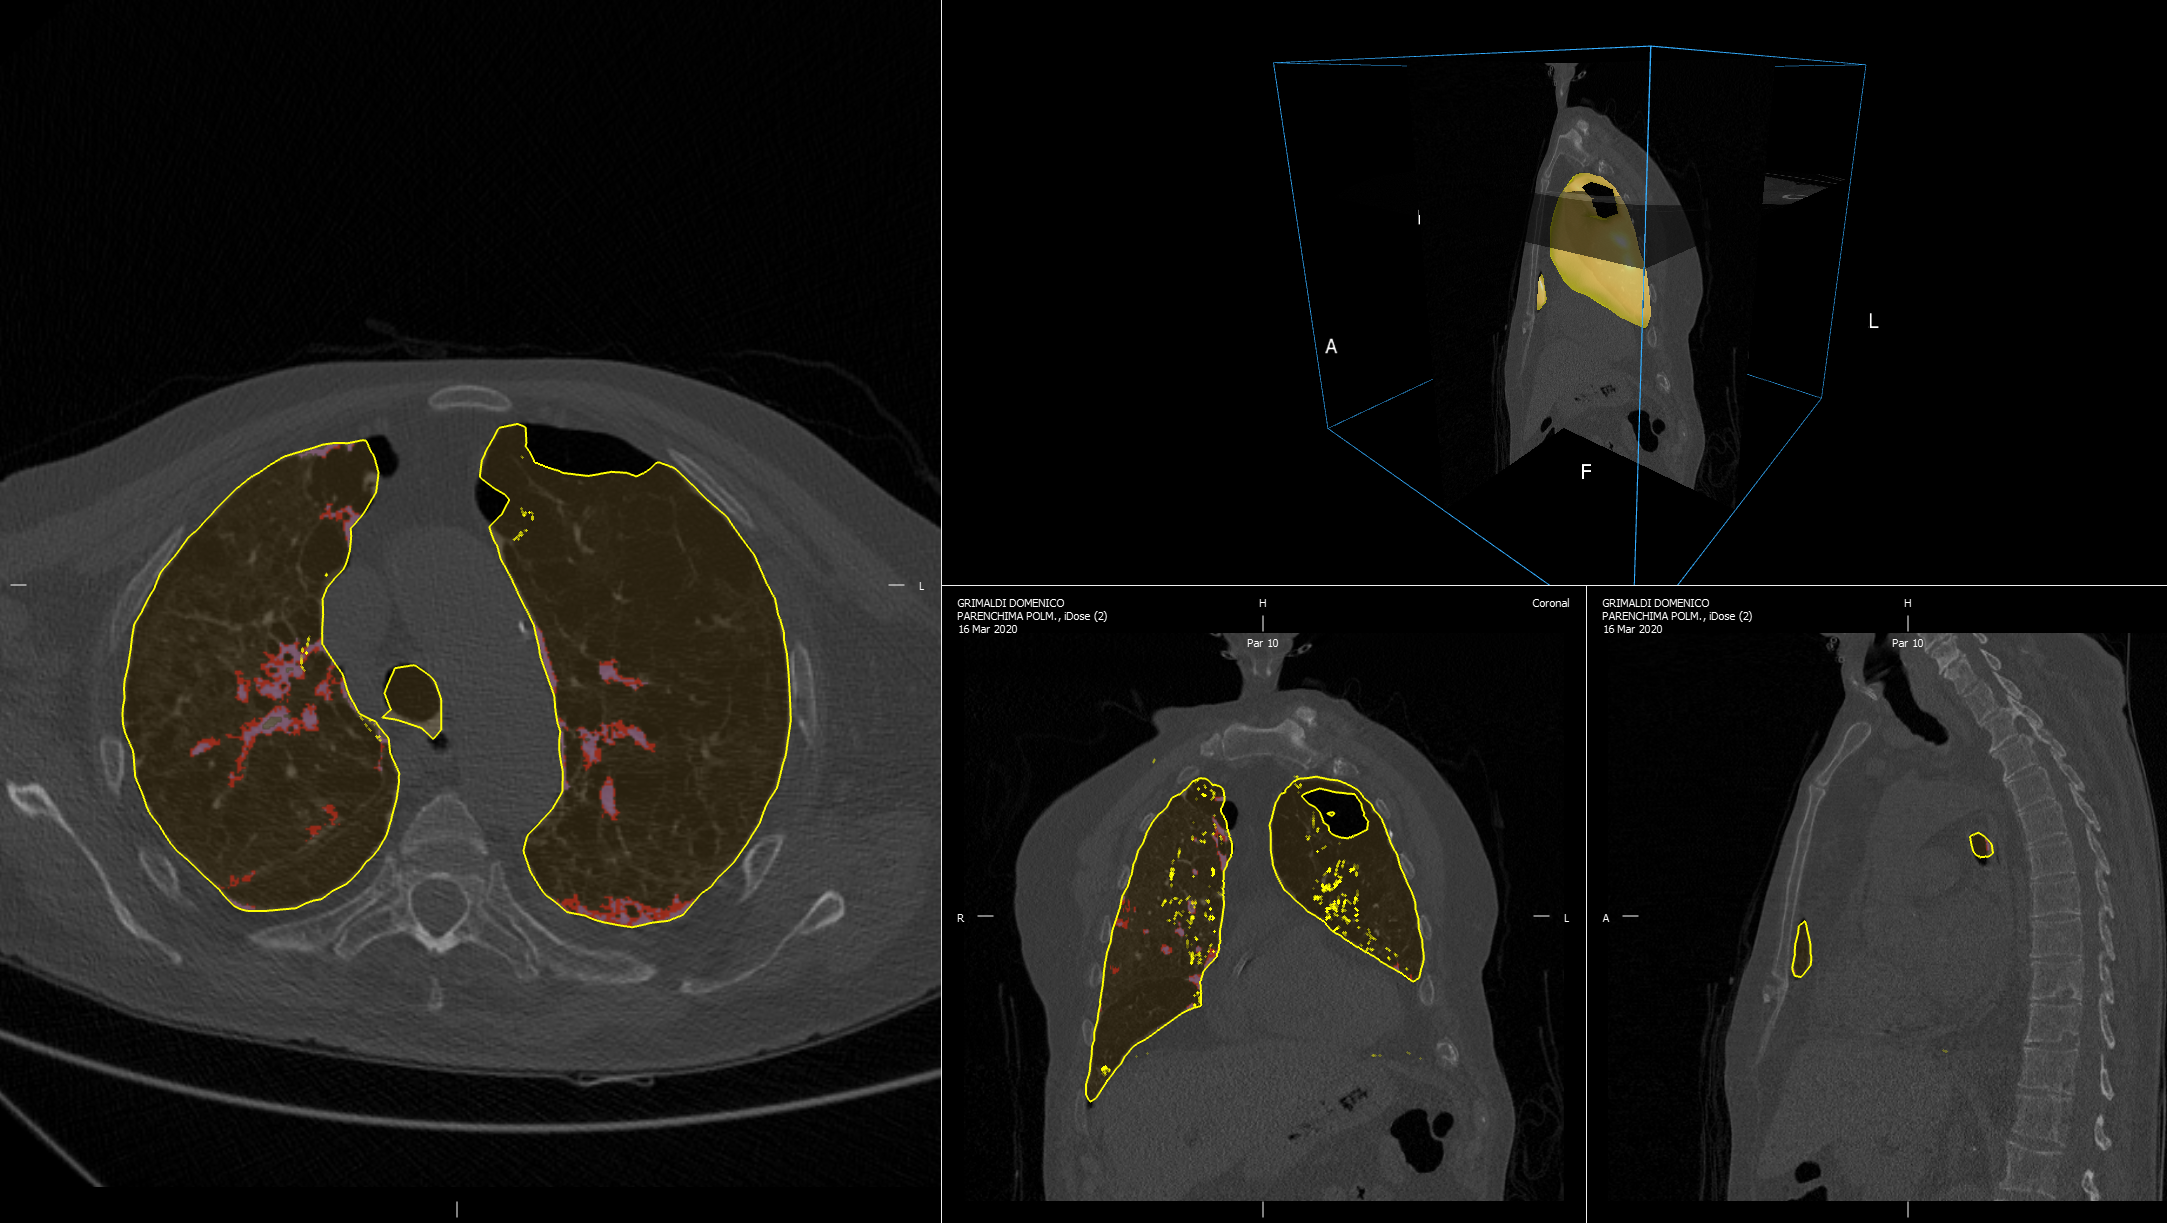
\includegraphics[width=\linewidth]{Bad_segm.png}\label{fig:badseg}}
	\newline
        \subfloat[][Example of segmentation classified as dubious ]{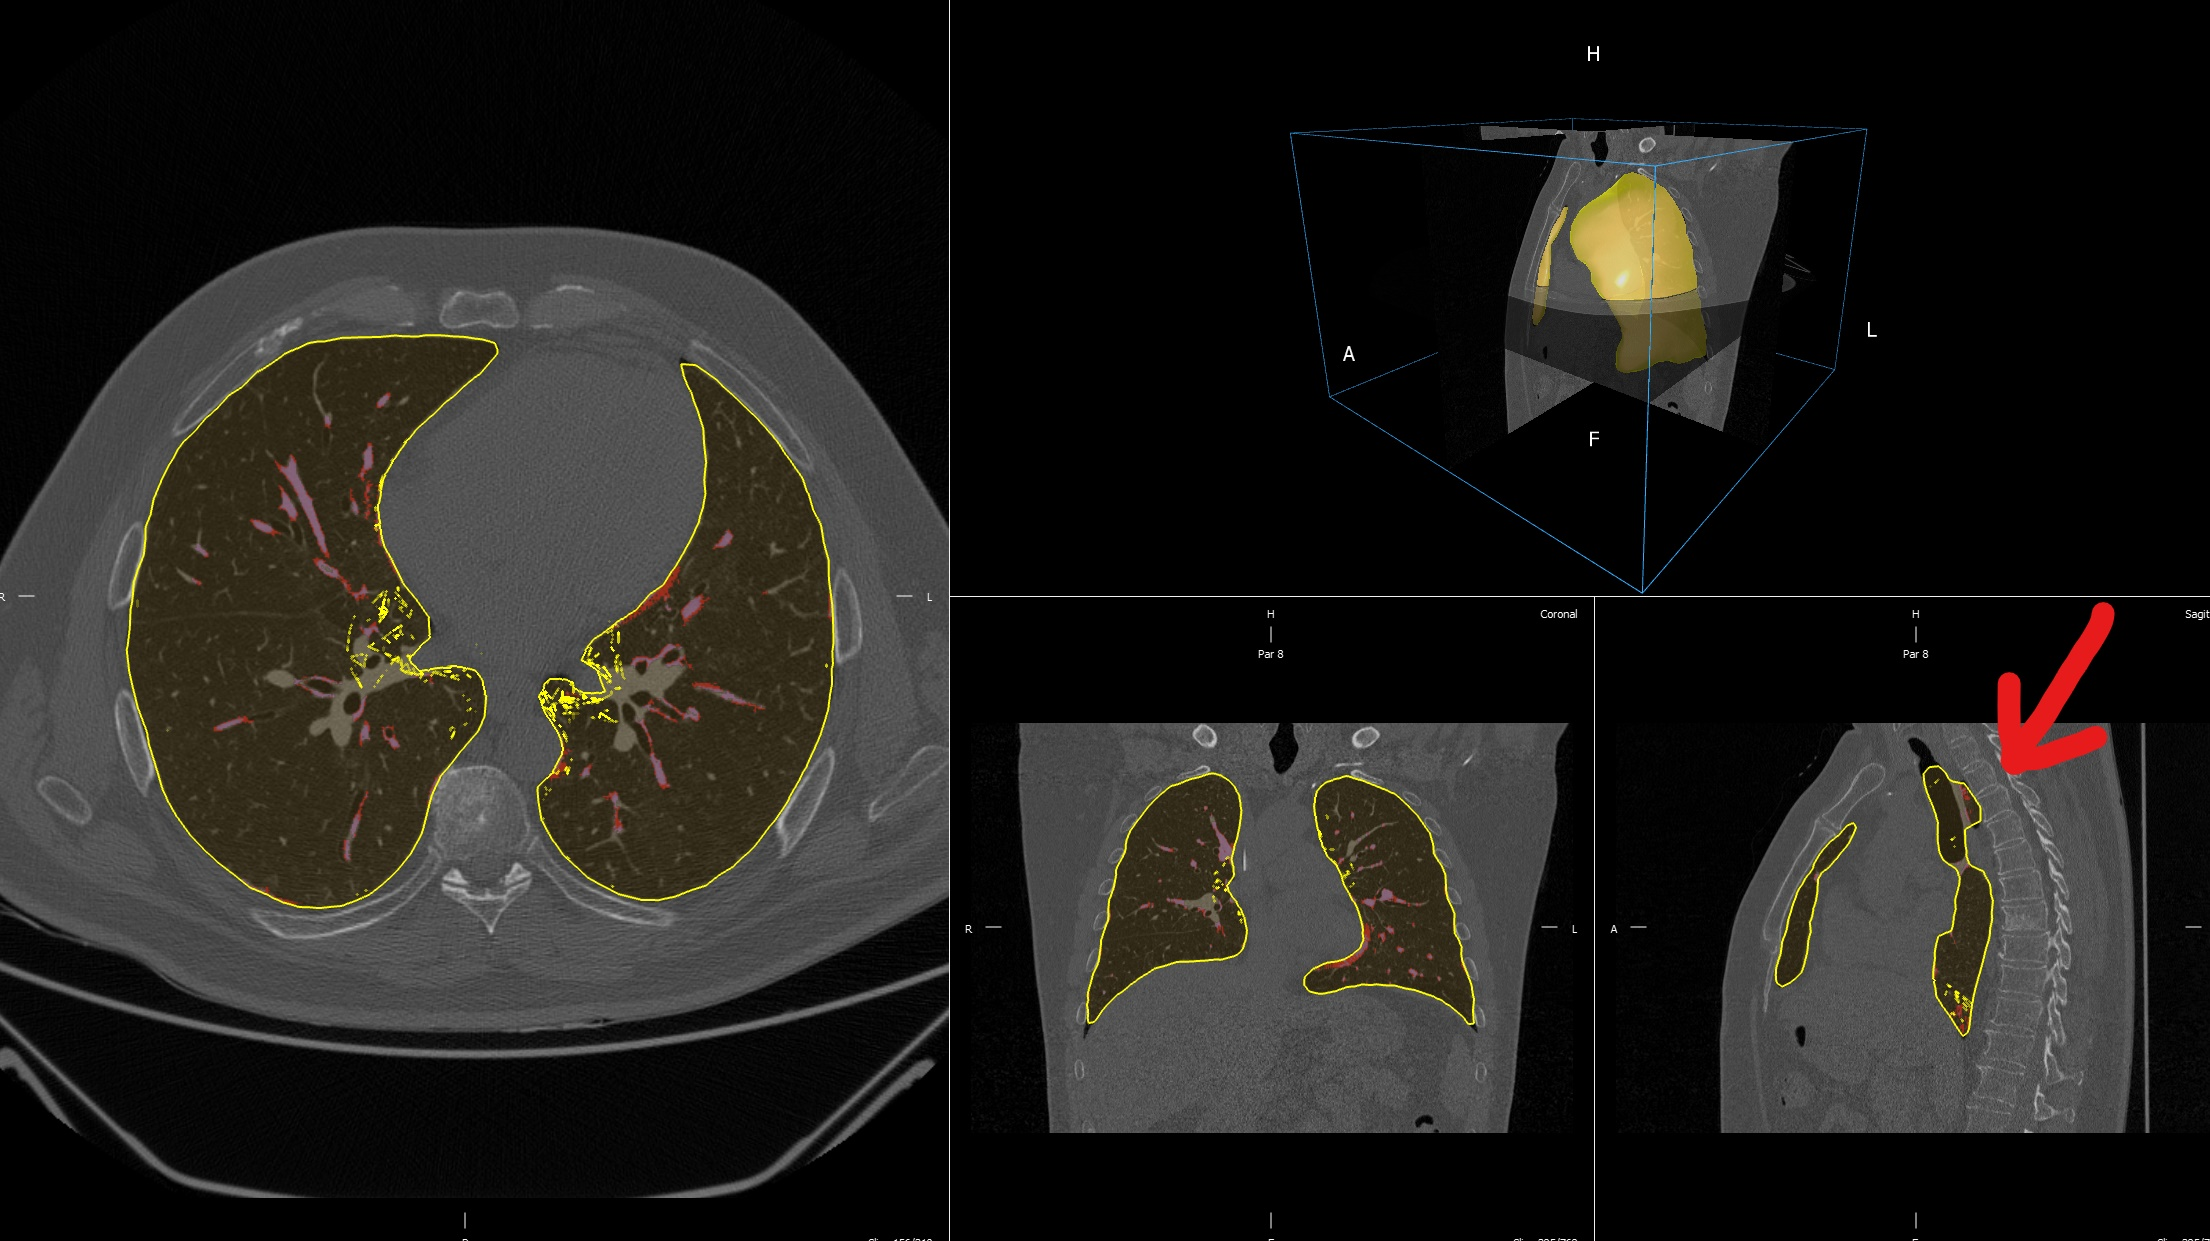
\includegraphics[width=\linewidth]{Dubiouos_segm.jpg}\label{fig:dubseg}}
        \caption{Example of segmentations being classified as bad (a) and dubious (b). In the first case (a) there is a clear hole in the lung which cannot be exact, in the second (b) there are small portion of outside tissue being labelled as lung as well as the whole trachea.}\label{fig:ExampleSeg}
\end{figure}

The result of this qualitative analysis can be seen in Table \ref{tab:ContingencyTableSegm} in which the incidence of both \death and \icu labels is computed in all possible segmentation categories.

\begin{table}
\centering
\caption{Contingency table with number of \death and \icu labels in all segmentation groups. \label{tab:ContingencyTableSegm}}
\begin{tabular}{llrrr}
\toprule
  & {} & \multicolumn{3}{l}{Subject} \\
  & Segmentation Status &     Bad & Good & Unsure \\
ICU Admission & Death &         &      &        \\
\midrule
0 & 0 &       8 &   11 &     24 \\
  & 1 &       5 &    0 &      6 \\
1 & 0 &       2 &    0 &      2 \\
  & 1 &       1 &    1 &      1 \\
\bottomrule
\end{tabular}
\end{table}

This table suggests that there is large difference of very severe individuals which end up being not perfectly segmented.
It's possible, even if unlikely, that the sample of analysed segmentations is biased in some way. However, given the numbers in Table \ref{tab:ContingencyTableSegm}, it can be reasonable to think that in some of the most important cases, which means those that correspond to 1 labels in \death or \icu, the values of the radiomic features used in this thesis were not the best possible. 

Another thing that can be noted is that in all models that included radiomics feature there are, among the important variables, features that quantify volumetric or shape information regarding the lung.

%A priori it's very difficult to imagine how lung size by itself could determine the prognosis of the patient.
It's possible that some of the most severe cases, which may need a more delicate and ad hoc handling during segmentation, end up being associated to lung shapes that are somewhat different from almost healthy patients.
In this light it's possible that the model is using these shape information, which is in some way altered with respect to reality, to infer the gravity of the situation and is finding something  because the information is somewhat unrealistic in the most severe cases.